% Options for packages loaded elsewhere
\PassOptionsToPackage{unicode}{hyperref}
\PassOptionsToPackage{hyphens}{url}
\PassOptionsToPackage{dvipsnames,svgnames,x11names}{xcolor}
%
\documentclass[
  letterpaper,
]{krantz}

\usepackage{amsmath,amssymb}
\usepackage{iftex}
\ifPDFTeX
  \usepackage[T1]{fontenc}
  \usepackage[utf8]{inputenc}
  \usepackage{textcomp} % provide euro and other symbols
\else % if luatex or xetex
  \usepackage{unicode-math}
  \defaultfontfeatures{Scale=MatchLowercase}
  \defaultfontfeatures[\rmfamily]{Ligatures=TeX,Scale=1}
\fi
\usepackage{lmodern}
\ifPDFTeX\else  
    % xetex/luatex font selection
\fi
% Use upquote if available, for straight quotes in verbatim environments
\IfFileExists{upquote.sty}{\usepackage{upquote}}{}
\IfFileExists{microtype.sty}{% use microtype if available
  \usepackage[]{microtype}
  \UseMicrotypeSet[protrusion]{basicmath} % disable protrusion for tt fonts
}{}
\makeatletter
\@ifundefined{KOMAClassName}{% if non-KOMA class
  \IfFileExists{parskip.sty}{%
    \usepackage{parskip}
  }{% else
    \setlength{\parindent}{0pt}
    \setlength{\parskip}{6pt plus 2pt minus 1pt}}
}{% if KOMA class
  \KOMAoptions{parskip=half}}
\makeatother
\usepackage{xcolor}
\setlength{\emergencystretch}{3em} % prevent overfull lines
\setcounter{secnumdepth}{5}
% Make \paragraph and \subparagraph free-standing
\ifx\paragraph\undefined\else
  \let\oldparagraph\paragraph
  \renewcommand{\paragraph}[1]{\oldparagraph{#1}\mbox{}}
\fi
\ifx\subparagraph\undefined\else
  \let\oldsubparagraph\subparagraph
  \renewcommand{\subparagraph}[1]{\oldsubparagraph{#1}\mbox{}}
\fi

\usepackage{color}
\usepackage{fancyvrb}
\newcommand{\VerbBar}{|}
\newcommand{\VERB}{\Verb[commandchars=\\\{\}]}
\DefineVerbatimEnvironment{Highlighting}{Verbatim}{commandchars=\\\{\}}
% Add ',fontsize=\small' for more characters per line
\usepackage{framed}
\definecolor{shadecolor}{RGB}{241,243,245}
\newenvironment{Shaded}{\begin{snugshade}}{\end{snugshade}}
\newcommand{\AlertTok}[1]{\textcolor[rgb]{0.68,0.00,0.00}{#1}}
\newcommand{\AnnotationTok}[1]{\textcolor[rgb]{0.37,0.37,0.37}{#1}}
\newcommand{\AttributeTok}[1]{\textcolor[rgb]{0.40,0.45,0.13}{#1}}
\newcommand{\BaseNTok}[1]{\textcolor[rgb]{0.68,0.00,0.00}{#1}}
\newcommand{\BuiltInTok}[1]{\textcolor[rgb]{0.00,0.23,0.31}{#1}}
\newcommand{\CharTok}[1]{\textcolor[rgb]{0.13,0.47,0.30}{#1}}
\newcommand{\CommentTok}[1]{\textcolor[rgb]{0.37,0.37,0.37}{#1}}
\newcommand{\CommentVarTok}[1]{\textcolor[rgb]{0.37,0.37,0.37}{\textit{#1}}}
\newcommand{\ConstantTok}[1]{\textcolor[rgb]{0.56,0.35,0.01}{#1}}
\newcommand{\ControlFlowTok}[1]{\textcolor[rgb]{0.00,0.23,0.31}{#1}}
\newcommand{\DataTypeTok}[1]{\textcolor[rgb]{0.68,0.00,0.00}{#1}}
\newcommand{\DecValTok}[1]{\textcolor[rgb]{0.68,0.00,0.00}{#1}}
\newcommand{\DocumentationTok}[1]{\textcolor[rgb]{0.37,0.37,0.37}{\textit{#1}}}
\newcommand{\ErrorTok}[1]{\textcolor[rgb]{0.68,0.00,0.00}{#1}}
\newcommand{\ExtensionTok}[1]{\textcolor[rgb]{0.00,0.23,0.31}{#1}}
\newcommand{\FloatTok}[1]{\textcolor[rgb]{0.68,0.00,0.00}{#1}}
\newcommand{\FunctionTok}[1]{\textcolor[rgb]{0.28,0.35,0.67}{#1}}
\newcommand{\ImportTok}[1]{\textcolor[rgb]{0.00,0.46,0.62}{#1}}
\newcommand{\InformationTok}[1]{\textcolor[rgb]{0.37,0.37,0.37}{#1}}
\newcommand{\KeywordTok}[1]{\textcolor[rgb]{0.00,0.23,0.31}{#1}}
\newcommand{\NormalTok}[1]{\textcolor[rgb]{0.00,0.23,0.31}{#1}}
\newcommand{\OperatorTok}[1]{\textcolor[rgb]{0.37,0.37,0.37}{#1}}
\newcommand{\OtherTok}[1]{\textcolor[rgb]{0.00,0.23,0.31}{#1}}
\newcommand{\PreprocessorTok}[1]{\textcolor[rgb]{0.68,0.00,0.00}{#1}}
\newcommand{\RegionMarkerTok}[1]{\textcolor[rgb]{0.00,0.23,0.31}{#1}}
\newcommand{\SpecialCharTok}[1]{\textcolor[rgb]{0.37,0.37,0.37}{#1}}
\newcommand{\SpecialStringTok}[1]{\textcolor[rgb]{0.13,0.47,0.30}{#1}}
\newcommand{\StringTok}[1]{\textcolor[rgb]{0.13,0.47,0.30}{#1}}
\newcommand{\VariableTok}[1]{\textcolor[rgb]{0.07,0.07,0.07}{#1}}
\newcommand{\VerbatimStringTok}[1]{\textcolor[rgb]{0.13,0.47,0.30}{#1}}
\newcommand{\WarningTok}[1]{\textcolor[rgb]{0.37,0.37,0.37}{\textit{#1}}}

\providecommand{\tightlist}{%
  \setlength{\itemsep}{0pt}\setlength{\parskip}{0pt}}\usepackage{longtable,booktabs,array}
\usepackage{calc} % for calculating minipage widths
% Correct order of tables after \paragraph or \subparagraph
\usepackage{etoolbox}
\makeatletter
\patchcmd\longtable{\par}{\if@noskipsec\mbox{}\fi\par}{}{}
\makeatother
% Allow footnotes in longtable head/foot
\IfFileExists{footnotehyper.sty}{\usepackage{footnotehyper}}{\usepackage{footnote}}
\makesavenoteenv{longtable}
\usepackage{graphicx}
\makeatletter
\def\maxwidth{\ifdim\Gin@nat@width>\linewidth\linewidth\else\Gin@nat@width\fi}
\def\maxheight{\ifdim\Gin@nat@height>\textheight\textheight\else\Gin@nat@height\fi}
\makeatother
% Scale images if necessary, so that they will not overflow the page
% margins by default, and it is still possible to overwrite the defaults
% using explicit options in \includegraphics[width, height, ...]{}
\setkeys{Gin}{width=\maxwidth,height=\maxheight,keepaspectratio}
% Set default figure placement to htbp
\makeatletter
\def\fps@figure{htbp}
\makeatother
\newlength{\cslhangindent}
\setlength{\cslhangindent}{1.5em}
\newlength{\csllabelwidth}
\setlength{\csllabelwidth}{3em}
\newlength{\cslentryspacingunit} % times entry-spacing
\setlength{\cslentryspacingunit}{\parskip}
\newenvironment{CSLReferences}[2] % #1 hanging-ident, #2 entry spacing
 {% don't indent paragraphs
  \setlength{\parindent}{0pt}
  % turn on hanging indent if param 1 is 1
  \ifodd #1
  \let\oldpar\par
  \def\par{\hangindent=\cslhangindent\oldpar}
  \fi
  % set entry spacing
  \setlength{\parskip}{#2\cslentryspacingunit}
 }%
 {}
\usepackage{calc}
\newcommand{\CSLBlock}[1]{#1\hfill\break}
\newcommand{\CSLLeftMargin}[1]{\parbox[t]{\csllabelwidth}{#1}}
\newcommand{\CSLRightInline}[1]{\parbox[t]{\linewidth - \csllabelwidth}{#1}\break}
\newcommand{\CSLIndent}[1]{\hspace{\cslhangindent}#1}

\renewcommand{\and}{\\}
\newtheorem{theorem}{Theorem}[chapter]
\newtheorem{exercise}{Exercise}[chapter]
\newtheorem{example}{Example}[chapter]
\newtheorem{definition}{Definition}[chapter]
%%\newtheorem{proof}{Proof}
\newenvironment{proof}[1][Proof]%
%  \topsep6\p@\@plus6\p@ \trivlist
{\par\addvspace{6pt}\normalfont {\bfseries #1}\hskip\labelsep\ignorespaces\itshape}
{\par\addvspace{6pt}}
\makeatletter
\makeatother
\makeatletter
\@ifpackageloaded{bookmark}{}{\usepackage{bookmark}}
\makeatother
\makeatletter
\@ifpackageloaded{caption}{}{\usepackage{caption}}
\AtBeginDocument{%
\ifdefined\contentsname
  \renewcommand*\contentsname{Table of contents}
\else
  \newcommand\contentsname{Table of contents}
\fi
\ifdefined\listfigurename
  \renewcommand*\listfigurename{List of Figures}
\else
  \newcommand\listfigurename{List of Figures}
\fi
\ifdefined\listtablename
  \renewcommand*\listtablename{List of Tables}
\else
  \newcommand\listtablename{List of Tables}
\fi
\ifdefined\figurename
  \renewcommand*\figurename{Figure}
\else
  \newcommand\figurename{Figure}
\fi
\ifdefined\tablename
  \renewcommand*\tablename{Table}
\else
  \newcommand\tablename{Table}
\fi
}
\@ifpackageloaded{float}{}{\usepackage{float}}
\floatstyle{ruled}
\@ifundefined{c@chapter}{\newfloat{codelisting}{h}{lop}}{\newfloat{codelisting}{h}{lop}[chapter]}
\floatname{codelisting}{Listing}
\newcommand*\listoflistings{\listof{codelisting}{List of Listings}}
\makeatother
\makeatletter
\@ifpackageloaded{caption}{}{\usepackage{caption}}
\@ifpackageloaded{subcaption}{}{\usepackage{subcaption}}
\makeatother
\makeatletter
\@ifpackageloaded{tcolorbox}{}{\usepackage[skins,breakable]{tcolorbox}}
\makeatother
\makeatletter
\@ifundefined{shadecolor}{\definecolor{shadecolor}{rgb}{.97, .97, .97}}
\makeatother
\makeatletter
\makeatother
\makeatletter
\makeatother
\ifLuaTeX
  \usepackage{selnolig}  % disable illegal ligatures
\fi
\IfFileExists{bookmark.sty}{\usepackage{bookmark}}{\usepackage{hyperref}}
\IfFileExists{xurl.sty}{\usepackage{xurl}}{} % add URL line breaks if available
\urlstyle{same} % disable monospaced font for URLs
\hypersetup{
  pdftitle={Model-based geostatistics for global public health using R},
  pdfauthor={Emanuele Giorgi; Claudio Fronterre},
  colorlinks=true,
  linkcolor={blue},
  filecolor={Maroon},
  citecolor={Blue},
  urlcolor={Blue},
  pdfcreator={LaTeX via pandoc}}

\title{Model-based geostatistics for global public health using R}
\author{Emanuele Giorgi \and Claudio Fronterre}
\date{2023-03-03}

\begin{document}
\maketitle
\ifdefined\Shaded\renewenvironment{Shaded}{\begin{tcolorbox}[sharp corners, boxrule=0pt, borderline west={3pt}{0pt}{shadecolor}, enhanced, breakable, interior hidden, frame hidden]}{\end{tcolorbox}}\fi

\renewcommand*\contentsname{Table of contents}
{
\hypersetup{linkcolor=}
\setcounter{tocdepth}{2}
\tableofcontents
}
\bookmarksetup{startatroot}

\hypertarget{preface}{%
\chapter*{Preface}\label{preface}}
\addcontentsline{toc}{chapter}{Preface}

\markboth{Preface}{Preface}

Its companion book ``Model-based geostatistical for global public
health'\,' by Peter J. Diggle (2019) is a strongly recommended
complementary read, as you work your way through this book.

\bookmarksetup{startatroot}

\hypertarget{introduction}{%
\chapter{Introduction}\label{introduction}}

The book provides shows how to carry out model-based geostatistical
analysis of public health data using the \texttt{RiskMap} R package. In
this introductory chapter, we explain what are the pre-requisites for
using this book and its learning objectives. We also explain what
software should be installed and how. Finally, we give a brief overview
of the class of models covered in this book, and the examples that will
be used to illustrate the methods and use of software.

\hypertarget{objectives-of-this-book}{%
\section{Objectives of this book}\label{objectives-of-this-book}}

The overall aim of this book is to provide you with the skills to
perform a geostatistical analysis of a data-set using the R software
environment. As you work your way through the book, you will learn to:

\begin{itemize}
\tightlist
\item
  explore geostatistical data-sets using graphical procedures and
  summary statistics;
\item
  formulate and fit geostatistical models using the maximum likelihood
  estimation method;
\item
  carry out prediction of health outcomes at different spatial scales;
\item
  visualize and interpret the results from geostatistical models;
\item
  model the relationships between spatially referenced risk factors and
  the health outcome of interest;
\item
  validate the assumptions of geostatistical models and assess their
  predictive performance.
\end{itemize}

Although the focus of this book is on public health, the statistical
ideas, as well as the software used, can also be applied for the
analysis of geostatistical data-sets arising from other scientific
fields.

\hypertarget{pre-requisites-for-using-this-book}{%
\section{Pre-requisites for using this
book}\label{pre-requisites-for-using-this-book}}

To effectively understand and use the material presented in this book,
it is expected that you should possess prior knowledge of basic
probability theory, foundational topics in statistical modelling and R
programming. Below we provide a more detailed explanation of the
pre-requisites for each of these three fields.

\hypertarget{topics-in-probability}{%
\subsection{Topics in probability}\label{topics-in-probability}}

Basics probability theory is important to fully understand the content
of this book. In particular, you should have knowledge of: the general
definition and properties of continuous and discrete distribution; how
the describe the properties of probability distributions through their
mean, variance and skeweness; the concepts of stochastic dependence and
correaltion; the distinction between marginal and conditional
distributions; the basic properties of the Gaussian, Binomial and
Poisson distributions; the definition and properties of the multivariate
Gaussian distribution. The redear can find an extensive explanation and
illustrations with examples of all these topics in Ross (2013).

\hypertarget{topics-in-statistics}{%
\subsection{Topics in statistics}\label{topics-in-statistics}}

Likelihood-based inference (whether frequensist or Bayesian) provides
the theoretical bedrock for the estimation of almost any statistical
model. In this book will focus on maximum likelihood estimation methods
of inference. Extensive use of the notions of point and interval
estimates obtained using the maximum likelihood estimation methods will
be made through the book. Recommended readings include chapters 1, 2 and
4 of Pawitan (2001).

Good prior knowledge of Generalized linear models (GLMs) is essential,
as the geostatistical modelling framework builds on these as an
extension. Before embarking on the use of this book, we thus encourage
you to review the basic theory of GLMs and, in particular, how these are
applied and interpreted. In this book, we will cover examples that will
model continuously measured outcomes and counts. Hence, good
understanding of linear regression modelling and modelling of counts
data using Binomial and Poisson regression should be the main focus of
the review. For comprehensive overview of GLMs and their implementation
in R, we refer you to Dobson and Barnett (2008).

\hypertarget{topics-in-r-programming}{%
\subsection{Topics in R programming}\label{topics-in-r-programming}}

Although this book does not require to possess advanced skills in R
programming, it is important you have good knowledge in the following
topics: creation and manipulation of vectors and matrices; logical
vectors; character vectors; handling of lists and data frame objects;
reading data into R; graphical procedures. A very large amount of freely
available material covering these topics can be found online. Our
recommendation is to start from the manual ``An introduction to R'' of
the Comprehensive R Archive Network available at this link, available at
\href{https://cran.r-project.org/manuals.html}{R manual}.

\hypertarget{obtaining-and-running-the-r-packages}{%
\section{Obtaining and running the R
packages}\label{obtaining-and-running-the-r-packages}}

It is advised that you obtain the latest 64-bit version of R in order to
run the R code of this book. To install R, go to the R website, where
you can download the installer packages for Windows and Mac, and find
instructions for Linux, using binary files.

\begin{itemize}
\tightlist
\item
  \href{https://cran.r-project.org/bin/windows/base/}{Windows}
\item
  \href{https://cran.r-project.org/bin/macosx}{Mac}
\item
  \href{https://cran.r-project.org/bin/linux}{Linux}
\end{itemize}

The list of the R packages used in this book is provided in
Table~\ref{tbl-packages}.

\hypertarget{tbl-packages}{}
\begin{longtable}[]{@{}
  >{\raggedright\arraybackslash}p{(\columnwidth - 2\tabcolsep) * \real{0.2917}}
  >{\raggedright\arraybackslash}p{(\columnwidth - 2\tabcolsep) * \real{0.7083}}@{}}
\caption{\label{tbl-packages}List of the R packages that will be used in
the book with a description of their use in the data analysis. The
packages marked by (E) are essential for the geostatistical analysis.
Those instead marked by (R) are recommended and can be helpful to
overcome issues as described under the column ``Used
for''.}\tabularnewline
\toprule\noalign{}
\begin{minipage}[b]{\linewidth}\raggedright
R packages
\end{minipage} & \begin{minipage}[b]{\linewidth}\raggedright
Used for
\end{minipage} \\
\midrule\noalign{}
\endfirsthead
\toprule\noalign{}
\begin{minipage}[b]{\linewidth}\raggedright
R packages
\end{minipage} & \begin{minipage}[b]{\linewidth}\raggedright
Used for
\end{minipage} \\
\midrule\noalign{}
\endhead
\bottomrule\noalign{}
\endlastfoot
\texttt{RiskMap} (E) & Estimating of geostatistical models and spatial
prediction \\
\texttt{sf} (E) & Handling of spatial data in R \\
\texttt{terra} (E) & Handling of raster files in R \\
\texttt{ggplot2} (E) & Creating maps and exploratory plots \\
\texttt{crsuggest} (R) & Guessing a coordinate reference systems when
unknown \\
\end{longtable}

To install packages in R for the first time, you can use the command
\texttt{install.packages} in the R console, as shown below for the
\texttt{RiskMap} package.

\begin{Shaded}
\begin{Highlighting}[]
\FunctionTok{install.packages}\NormalTok{(}\StringTok{"RiskMap"}\NormalTok{)}
\end{Highlighting}
\end{Shaded}

\hypertarget{sec-examples-ch1}{%
\section{Data-sets used in the book}\label{sec-examples-ch1}}

The geostatistical data-sets described in this section will be used
throughout the book to illustrate the use of the R packages mentioned in
the previous sections.

Each of the examples data-sets can be loaded from the \texttt{RiskMap}
package, using the command

\begin{Shaded}
\begin{Highlighting}[]
\FunctionTok{data}\NormalTok{(NAME\_OF\_THE\_DATASET)}
\end{Highlighting}
\end{Shaded}

where in place of \texttt{NAME\_OF\_THE\_DATASET} you should type of the
name of one of the data-sets listed in Table~\ref{tbl-data-sets}.

\hypertarget{tbl-data-sets}{}
\begin{longtable}[]{@{}
  >{\raggedright\arraybackslash}p{(\columnwidth - 4\tabcolsep) * \real{0.2466}}
  >{\raggedright\arraybackslash}p{(\columnwidth - 4\tabcolsep) * \real{0.5068}}
  >{\raggedright\arraybackslash}p{(\columnwidth - 4\tabcolsep) * \real{0.2466}}@{}}
\caption{\label{tbl-data-sets}List of data-sets available from the
\texttt{RiskMap} package. Data-sets listed as ``Example'' are used
throughout the book to illustrate the use of R functions. Data-sets
listed as ``Case study'' are analysed in
Chapter~\ref{sec-case-studies}.}\tabularnewline
\toprule\noalign{}
\begin{minipage}[b]{\linewidth}\raggedright
Names of the data-set
\end{minipage} & \begin{minipage}[b]{\linewidth}\raggedright
Short description
\end{minipage} & \begin{minipage}[b]{\linewidth}\raggedright
Used in this book as
\end{minipage} \\
\midrule\noalign{}
\endfirsthead
\toprule\noalign{}
\begin{minipage}[b]{\linewidth}\raggedright
Names of the data-set
\end{minipage} & \begin{minipage}[b]{\linewidth}\raggedright
Short description
\end{minipage} & \begin{minipage}[b]{\linewidth}\raggedright
Used in this book as
\end{minipage} \\
\midrule\noalign{}
\endhead
\bottomrule\noalign{}
\endlastfoot
\texttt{galicia} & Lead concentration m from moss samples collected in
Galicia, Northern Spain & Example \\
\texttt{liberia} & Prevalence data on river-blindness from Liberia &
Example \\
\texttt{malkenya} & Malaria prevalence data from a community and school
survey conducted in Western Kenya & Example \\
\texttt{italy\_sim} & Simulated geostatistical data-set within the
Italian national boundaries & Example \\
\texttt{malnutrition} & Data on stunting among children in Ghana & Case
study \\
\end{longtable}

\hypertarget{lead-concentration-in-galicia}{%
\subsection{Lead concentration in
Galicia}\label{lead-concentration-in-galicia}}

\begin{figure}

{\centering 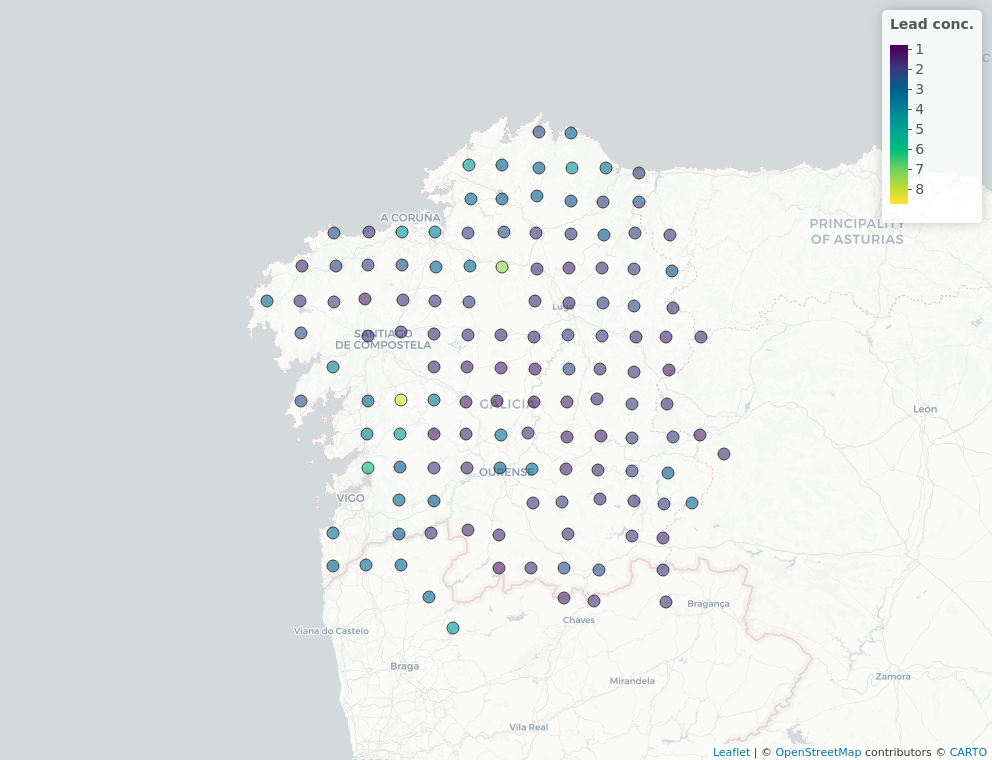
\includegraphics[width=3.31in,height=\textheight]{./figures/galicia_ch1.png}

}

\caption{\label{fig-galicia-ch1}Data on the meausred lead concentration
(in micrograms per gram dry weight) in moss samples collected in
Galicia, North-West of Spain.}

\end{figure}

Lead is a heavy metal which, in high concentrations, can cause chronic
damage to living organisms over a long period of time. For this reason
its spread and source must be regularly monitored. To assess the extent
of the contamination in an area, measurements of lead are often taken
from plants. The data here considered (Figure~\ref{fig-galicia-ch1})
consist of 132 locations of moss samples collected in 2000, in and
around Galicia, a region in the North-Western part of Spain. One of the
objectives of this survey was to establish the spatial pattern of lead
concentration in Galicia so as to better identify possible sources of
contamination; fore more information, see Fernández, Rey, and
Carballeira (2000).

In this case, geostatistical modelling can be used to predict the lead
concentration across Galicia and allows to disentangle variation which
is purely random, possibly due to measurement error, and genuine spatial
variation, which is our main object of interest.

This data-set will be used in this book to show how to carry out the
spatial analysis of continuously measured variables using linear
geostatistical models.

\hypertarget{sec-rb-ch1}{%
\subsection{River-blindness in Liberia}\label{sec-rb-ch1}}

\begin{figure}

{\centering 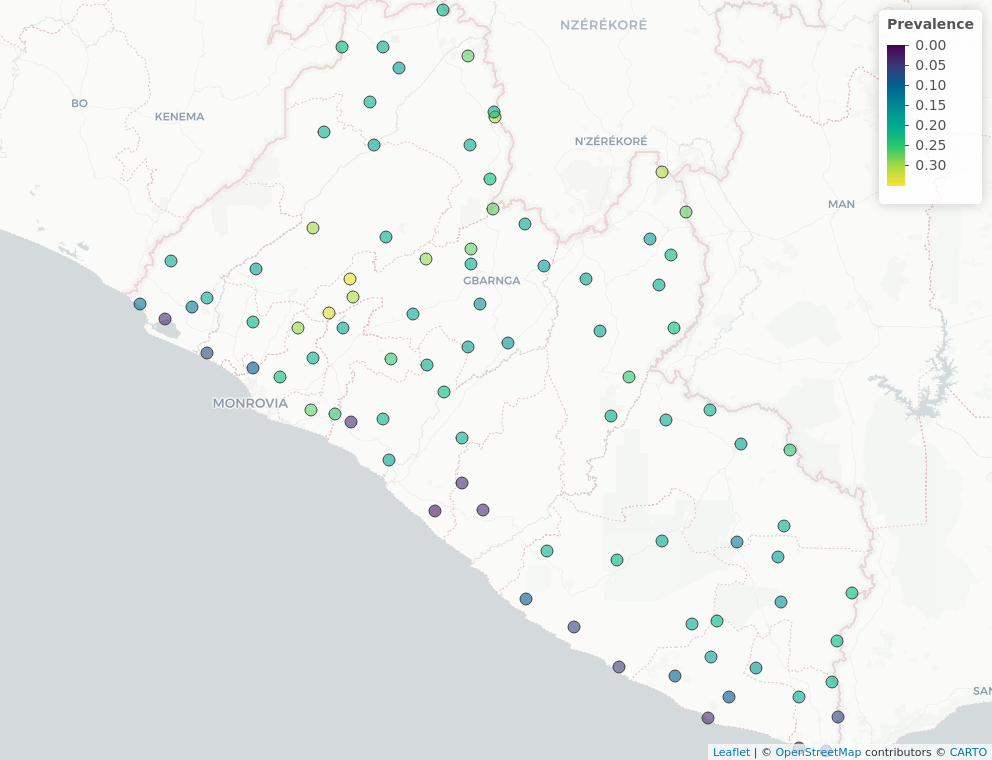
\includegraphics[width=3.31in,height=\textheight]{./figures/liberia_ch1.png}

}

\caption{\label{fig-liberia-ch1}River-blindness data from a
cross-sectional survey carried out in Liberia.}

\end{figure}

In low-resource settings, where disease registries are typically absent,
cross-sectional surveys are an essential monitoring tool that enables
the estimation of the disease burden in a population of interest. The
data considered in this example (Figure~\ref{fig-liberia-ch1}) have been
collected as part of an Africa-wide initiative called the Rapid
Epidemiological Mapping of Onchocerchiasis (REMO) carried out in 2011 in
20 African countries (Zouré et al. 2014). The goal of REMO is to
identify areas where river-blindness (or onchocerchiasis), a disease
transmitted by black flies who breed along fast flowing rivers, is still
a public health problem. In this context, it is especially of interest
to identify communities with a prevalence above 20\% and for treatment
is urgently needed.

In this book, we will use data collected from Liberia to model nodule
prevalence, which is based on a alternative and cheaper diagnostic
technique for river-blindness. In the analysis of this data-set, we will
illustrate how to formulate and fit Binomial geostatistical models, and
how these can be used to predict prevalence within a region of interest.

\hypertarget{sec-malaria-ch1}{%
\subsection{Malaria in the Western Kenyan
Highlands}\label{sec-malaria-ch1}}

\begin{figure}

{\centering 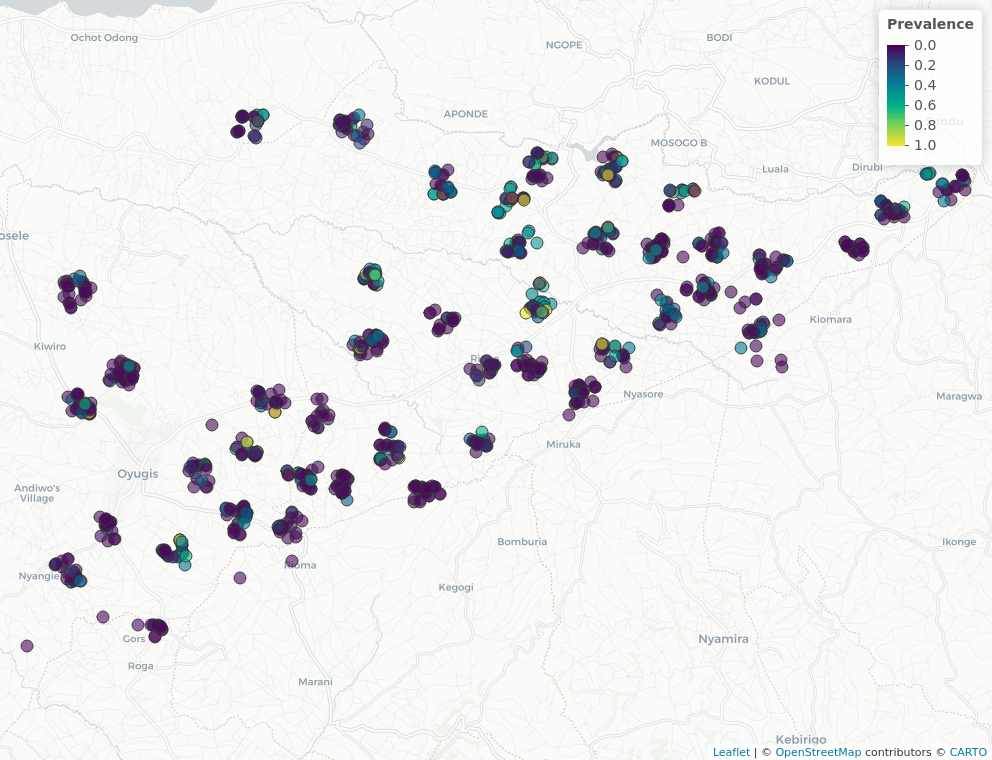
\includegraphics[width=3.31in,height=\textheight]{./figures/malkenya_ch1.png}

}

\caption{\label{fig-malkenya-ch1}Malaria prevalence data from a
cross-sectional survey carried out in Nyanza Province, in the Western
Highlands of Kenya.}

\end{figure}

Malaria is one of deadliest diseases that affects populations living in
tropical and subtropical countries. It is caused by a parasite of the
genus Plasmodium which is transmitted through the infectious bite of
female Anopheles mosquitoes. In the following chapters, we shall analyse
a data-set from a cross-sectional community survey carried out in July
2010 in Nyanza Province, in the Western Highlands of Kenya (Stevenson
2013).

What distinguishes this from the other examples data-sets is that the
data contain both individual-level and household-level information. The
outcome of interest is the result from a rapid diagnostic test for
malaria which. In the book, we will illustrate how to account for the
the hierarchical structure of the data and the binary nature of the
outcome at each of the stages of the geostatistical analysis.

\hypertarget{sec-mosq-data-ch1}{%
\subsection{\texorpdfstring{\emph{Anopheles gambiae} mosquitoes in
Southern
Cameroon}{Anopheles gambiae mosquitoes in Southern Cameroon}}\label{sec-mosq-data-ch1}}

\begin{figure}

{\centering 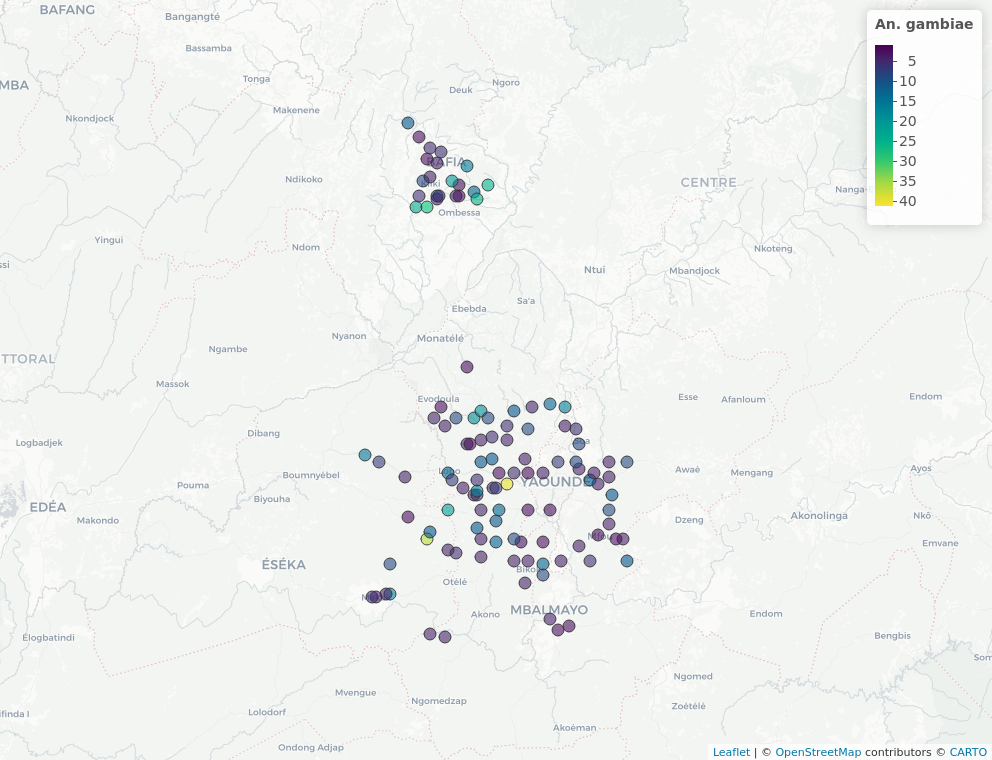
\includegraphics[width=3.31in,height=\textheight]{./figures/anopheles_ch1.png}

}

\caption{\label{fig-anopheles-ch1}Map of the collected number of
\emph{Anopheles gambiae} mosquitoes in an area of Southern Cameroon.}

\end{figure}

In studies of vector-borne and zoonotic diseases, understanding of the
vector distribution can help to better guide the decision-making process
for the implementation, monitoring and evaluation of control programmes.
\emph{Anopheles gambiae} mosquitoes are one of the main vectors for
malaria transmission in sub-Saharan Africa. Their distribution over
space is affected by several environmental and climatic factors,
including temperature, humidity and vegetation.

The data-set on mosquitoes (Figure~\ref{fig-anopheles-ch1}) that will
use in the book consists of a sub-set taken from a large database (Tene
Fossog et al. 2015). This was assembled in order to understand how the
environment affects the distribution of different species of
\emph{Anopheles} mosquitoes in sub-Saharan Africa. This example data-set
will be used to illustrate the application of Poisson geostatistical
models for mapping mosquitoes abundance.

\hypertarget{sec-italy-sim-data-ch1}{%
\subsection{Simulated-dataset}\label{sec-italy-sim-data-ch1}}

\begin{figure}

{\centering 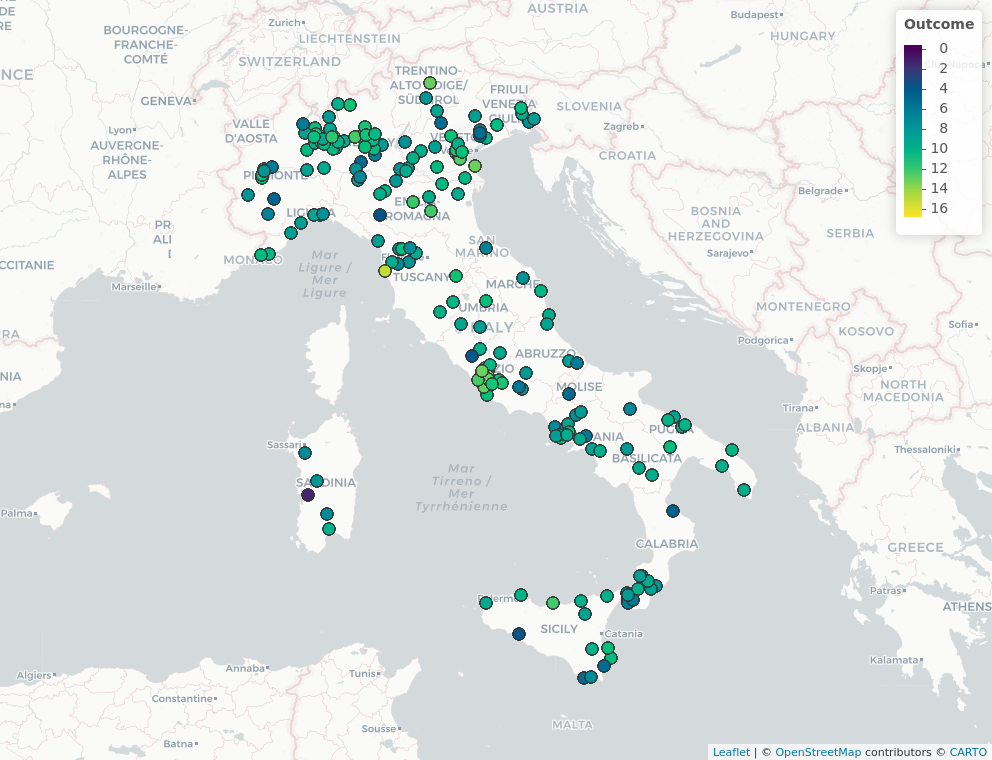
\includegraphics[width=3.31in,height=\textheight]{./figures/italy_sim_ch1.png}

}

\caption{\label{fig-italy-sim-ch1}Map of the locations of the simulated
data-set generated over Italy for a continuous outcome.}

\end{figure}

This data-set was generated using a geostatistical model, with the
addition of unstructured random effects at provincial and regional
level. More details on how this data-set was generated will be provided
in Section~\ref{sec-linear-model}. Whilst this data-set does not have
any scientific relevance like the other data-sets used in this book, it
will serve us to illustrate some of the more advanced features of the
package that enable the inclusion of random effects, in addition to the
latent Gaussian process that is common to all geostatistical models. The
skills you will aquire through the analysis of this data-set will be
useful for the analysis of data-sets presented as case studies in
Chapter~\ref{sec-case-studies}.

\hypertarget{sec-geostat-models}{%
\section{Geostatistical problems and geostatistical
models}\label{sec-geostat-models}}

What the examples of the previous section have in common is that, in
each case, the goal of statistical analysis is to draw inferences on an
unobserved spatially continuous surface using data collected from a
finite set of locations. The lead concentration in Galicia, the
prevalence for river-blindness in Liberia and the abundance of \emph{A.
gambiae} mosquitoes in Cameroon can all be represented as spatially
continuous processes that originate from the combined effects of
environmental factors. We denote this class of inferential problems as
\emph{geostatistical problems} for which a solution can be found through
the development and application of suitable \emph{geostatistical
models}, which are the subject of this book.

As one can soon realize, geostatistical problems are not unique to
global health but arise in many other fields of science, including
economics, physics, biology, geology and others. It thus comes to no
surprise that geostatistics was initially developed in the South African
mining industry in the 1950s (Krige 1951). This was then further
developed as a self-contained discipline by Georges Matheron and other
researchers at Fontainebleau, in France (Matheron 1963; Chilès and
Delfiner 2016). In Watson (1971) and Watson (1972) a first connection is
drawn between geostatistics and the prediction of stochastic processes.
However, it is only with Ripley (1981) and then Cressie (1991) that
geostatistics is explicitly brought into a classical statistical
framework for the analysis of spatially referenced data. P. J. Diggle,
Tawn, and Moyeed (1998) coined the term \emph{model-based geostastics}
and introduced this as belonging to the general class of generalized
linear mixed models (Breslow and Clayton 1993), while emphasizing the
use of likelihood-based methods of inference. As in P. J. Diggle, Tawn,
and Moyeed (1998), also in this book, we advocate the application of
model-based geostistical models as a class of parametric statistical
models on which inference can be carried out using either maximum
likelihood estimation or Bayesian methods.

More precisely, our attention will be directed at the class of
\emph{generalized linear geostatistical models}, or GLGM. To formally
specify this, we first define the random variables \(S\), a spatial
stochastic process, and the random variable \(Y= (Y_1, \ldots, Y_n)\)
which correspond to the outcome observed at a set of locations
\(X = (x_1, \ldots, x_n)\). Let us use \([A]\) to denote ``the
distribution of the random variable \(A\)''. To formulate a GLGM, we
should then specify the joint distribution of \(S\) and \(Y\), which we
write as

\begin{equation}\protect\hypertarget{eq-glgm-joint-ch1}{}{
[Y, S] = [S] [Y | S].
}\label{eq-glgm-joint-ch1}\end{equation}

On the right-hand side of the equation above, we have factorized the
joint distribution of \(Y\) and \(S\), as the product between the
marginal distribution of \(S\) and the conditional distribution of \(Y\)
given \(S\). Hence, the formulation of a GLGM can be break down into the
tasks of formulating \([S]\) and \([Y | S]\).

In defining \([S]\), throughout the book, we shall assume that this is a
zero-mean stationary and isotropic Gaussian process. In other words,
these assumptions impose that the joint distribution of
\(S(X) = (S(x_1),\ldots,S(x_n))\), i.e.~the process \(S\) at the sampled
locations \(x_1, \ldots, x_n\), is invariant with respect to rations and
translations of the locations \(X\). In practical terms, the main
implication of this is that, for any pair of locations \(x_i\) and
\(x_j\) the correlation function \(\rho(\cdot)\) between \(S(x_i)\) and
\(S(x_j)\) is purely a function of the Euclidean distance, \(u_{ij}\),
between \(x_i\) and \(x_j\),
i.e.~\begin{equation}\protect\hypertarget{eq-correlation-ch1}{}{
{\rm cov}\{S(x_i), S(x_j)\} = \sigma^2\rho(u_{ij}),
}\label{eq-correlation-ch1}\end{equation}

where \(\sigma^2\) is the variance of \(S(x)\) for all \(x\). Below we
provide more details on the type of covoriance functions that we
consider in this book. Furthermore, the fact that we assume the process
\(S\) to have mean zero is because this is process acts as a residual
term in our modelling of \(Y\). This aspect will be reiterated several
times in the following chapters, as it as important implications for the
interpretation of the other components of a geostatistical model, as
well understanding the results of the analysis.

Finally, we model \([Y | S]\), i.e.~the distribution of \(Y\) given
\(S\), is modeled as a set of mutually independent distributions which
belong the exponential family, as defined in classical generalized
linear modelling framework (Nelder and Wedderburn 1972). It then follows
that, we can write \([Y | S]\) as

\begin{equation}\protect\hypertarget{eq-glm-ch1}{}{
[Y | S] = \prod_{i=1}^n [Y_i | S(x_i)].
}\label{eq-glm-ch1}\end{equation}

The final step then consists of specifying a distribution for
\([Y_i | S(x_i)]\). Table~\ref{tbl-glm} gives the range, mean and
variance the three specifications for \${[}Y\_i \textbar{}
S(x\_i){]}\$\$ which we will consider in this book. In
Table~\ref{tbl-glm}, the \emph{canonical function}, say \(g(\cdot)\),
denotes the natural transformation of the mean component \(\mu_i\) that
allows us to introduce both covariates and the spatial process
\(S(x_i)\) into the model so as to explain the variation in \(\mu_i\) as

\begin{equation}\protect\hypertarget{eq-linear-predictor-ch1}{}{
g(\mu_i) = d(x_i)^\top \beta + S(x_i).
}\label{eq-linear-predictor-ch1}\end{equation}

where \(d(x_i)\) is a vector of spatially referenced covariates with
associated regression coefficients \(\beta\). Finally, the quantity
\(m_i\), which appears in the formulation of the Binomial and Poisson
distributions, is an offset quantity and is used to account for the
number of \emph{tests} or the population size at a given location
\(x_i\).

\hypertarget{tbl-glm}{}
\begin{longtable}[]{@{}
  >{\raggedright\arraybackslash}p{(\columnwidth - 8\tabcolsep) * \real{0.2000}}
  >{\raggedright\arraybackslash}p{(\columnwidth - 8\tabcolsep) * \real{0.2000}}
  >{\raggedright\arraybackslash}p{(\columnwidth - 8\tabcolsep) * \real{0.2000}}
  >{\raggedright\arraybackslash}p{(\columnwidth - 8\tabcolsep) * \real{0.2000}}
  >{\raggedright\arraybackslash}p{(\columnwidth - 8\tabcolsep) * \real{0.2000}}@{}}
\caption{\label{tbl-glm}Type of outcomes \(Y_{i}\) considered in this
book.}\tabularnewline
\toprule\noalign{}
\begin{minipage}[b]{\linewidth}\raggedright
Distribution
\end{minipage} & \begin{minipage}[b]{\linewidth}\raggedright
Range of \(Y_i\)
\end{minipage} & \begin{minipage}[b]{\linewidth}\raggedright
Mean of \([Y_i | S(x_i)]\)
\end{minipage} & \begin{minipage}[b]{\linewidth}\raggedright
Variance of \([Y_i | S(x_i)]\)
\end{minipage} & \begin{minipage}[b]{\linewidth}\raggedright
Canonical link
\end{minipage} \\
\midrule\noalign{}
\endfirsthead
\toprule\noalign{}
\begin{minipage}[b]{\linewidth}\raggedright
Distribution
\end{minipage} & \begin{minipage}[b]{\linewidth}\raggedright
Range of \(Y_i\)
\end{minipage} & \begin{minipage}[b]{\linewidth}\raggedright
Mean of \([Y_i | S(x_i)]\)
\end{minipage} & \begin{minipage}[b]{\linewidth}\raggedright
Variance of \([Y_i | S(x_i)]\)
\end{minipage} & \begin{minipage}[b]{\linewidth}\raggedright
Canonical link
\end{minipage} \\
\midrule\noalign{}
\endhead
\bottomrule\noalign{}
\endlastfoot
Gaussian & \((-\infty, +\infty)\) & \(\mu_i\) & \(\tau^2\) &
\(g(\mu_i) = \mu_i\) \\
Binomial & \(1,\dots,m_i\) & \(m_i\mu_i\) & \(m_i\mu_i(1-\mu_i)\) &
\(g(\mu_i) = \log\{ \mu_i/(1-\mu_i) \}\) \\
Poisson & \(1,2,\ldots,\infty\) & \(m_i\mu_i\) & \(m_i\mu_i\) &
\(g(\mu_i) = \log\{ \mu_i \}\) \\
\end{longtable}

Based on the formulation in (\ref{eq-linear-predictor-ch1}), we can see
that \(S(x_i)\) quantifies residual spatial effects on \(\mu_i\) that
have not been accounted for by the covariates \(d(x_i)\). In an ideal
scenario, the covariates \(d(x_i)\) should explain all the spatial
variation without the need for \(S(x_i)\). Although this unrealistic, in
practice we may be able to most of the variation in \(\mu_i\) through
\(d(x_i)\) and, hence, reduce \(S(x_i)\) to a negligible component. In
Chapter 2, we will show how a thorough exploratory analysis can help to
understand whether we have come close to that ideal scenario or, if
instead, we need the use of GLGM to model the data.

The model described in (\ref{eq-linear-predictor-ch1}) can be seen as
the most basic GLGM that can be used for a geostatistical analysis. As
we will see in the analysis of some of the examples and, in Chapter 6,
for the case studies, extensions of this model will be required to
accommodate the intrinsic non-spatial random variation of the data which
is not captured by the covariates.

The types of problems that statistical models are applied to can be
distinguished into three main categories: prediction problems;
explanatory problems; problems of hypothesis testing. Most of the times,
geostatistical problems tend to fall under the first category, where the
goal is make predictive inferences on the process \(S(x)\) at location
\(x\), which is usually outside of the set of sampled locations.
However, as will illustrate in the later chapters, geostatistical models
play an important also in the other two types of problems. In
particular, we will show that spatial correlation can have a substantial
impact on the point estimates and standard errors for \(\beta\). Hence,
if the goal of the analysis is explain the relationship between a
covariate \(d(x)\) with the mean component \(\mu\).

\hypertarget{sec-matern-correlation}{%
\subsection{The Matern family of correlation
functions}\label{sec-matern-correlation}}

Throughout the book, we shall consider the Matern (2013) family of
correlation functions to model the spatial correlation of the Gaussian
process \(S(x)\). This defined as
\begin{equation}\protect\hypertarget{eq-matern}{}{
\rho(u;\phi,\kappa) =\{2^{\kappa-1} \Gamma(\kappa)\}^{-1} (u/\phi)^\kappa K_\kappa(u/\phi),
}\label{eq-matern}\end{equation} where \(\phi>0\) and \(\kappa>0\) are
parameters and \(K_\kappa(\cdot)\) is the modified Bessel function of
the third kind of order \(\kappa\). The parameters \(\phi\) and
\(\kappa\) regulate how fast the spatial correlation decays to zero for
increasing distance and the smoothness of the process, respectively. A
special case of Matern family of correlation functions, which is
obtained when \(\kappa=0.5\), will be of particular relevance to the
application considered in this book. This is the expeonential
correlation function which we write as
\begin{equation}\protect\hypertarget{eq-exp}{}{
\rho(u;\phi) = \exp\{-u/\phi\}.
}\label{eq-exp}\end{equation}

Another special case, which we dot consider in this book but has often
been used in machine learning applications, is the Gaussian correlation
function obtain as a limiting case for \(\kappa \to +\infty\) the
possible smoothest process arising from the Matern family.

To better understand how \(\phi\) and \(\kappa\) affect the spatial
correlation and the pattern of the spatial of the spatial surface, we
now consider some examples.

\begin{figure}

{\centering 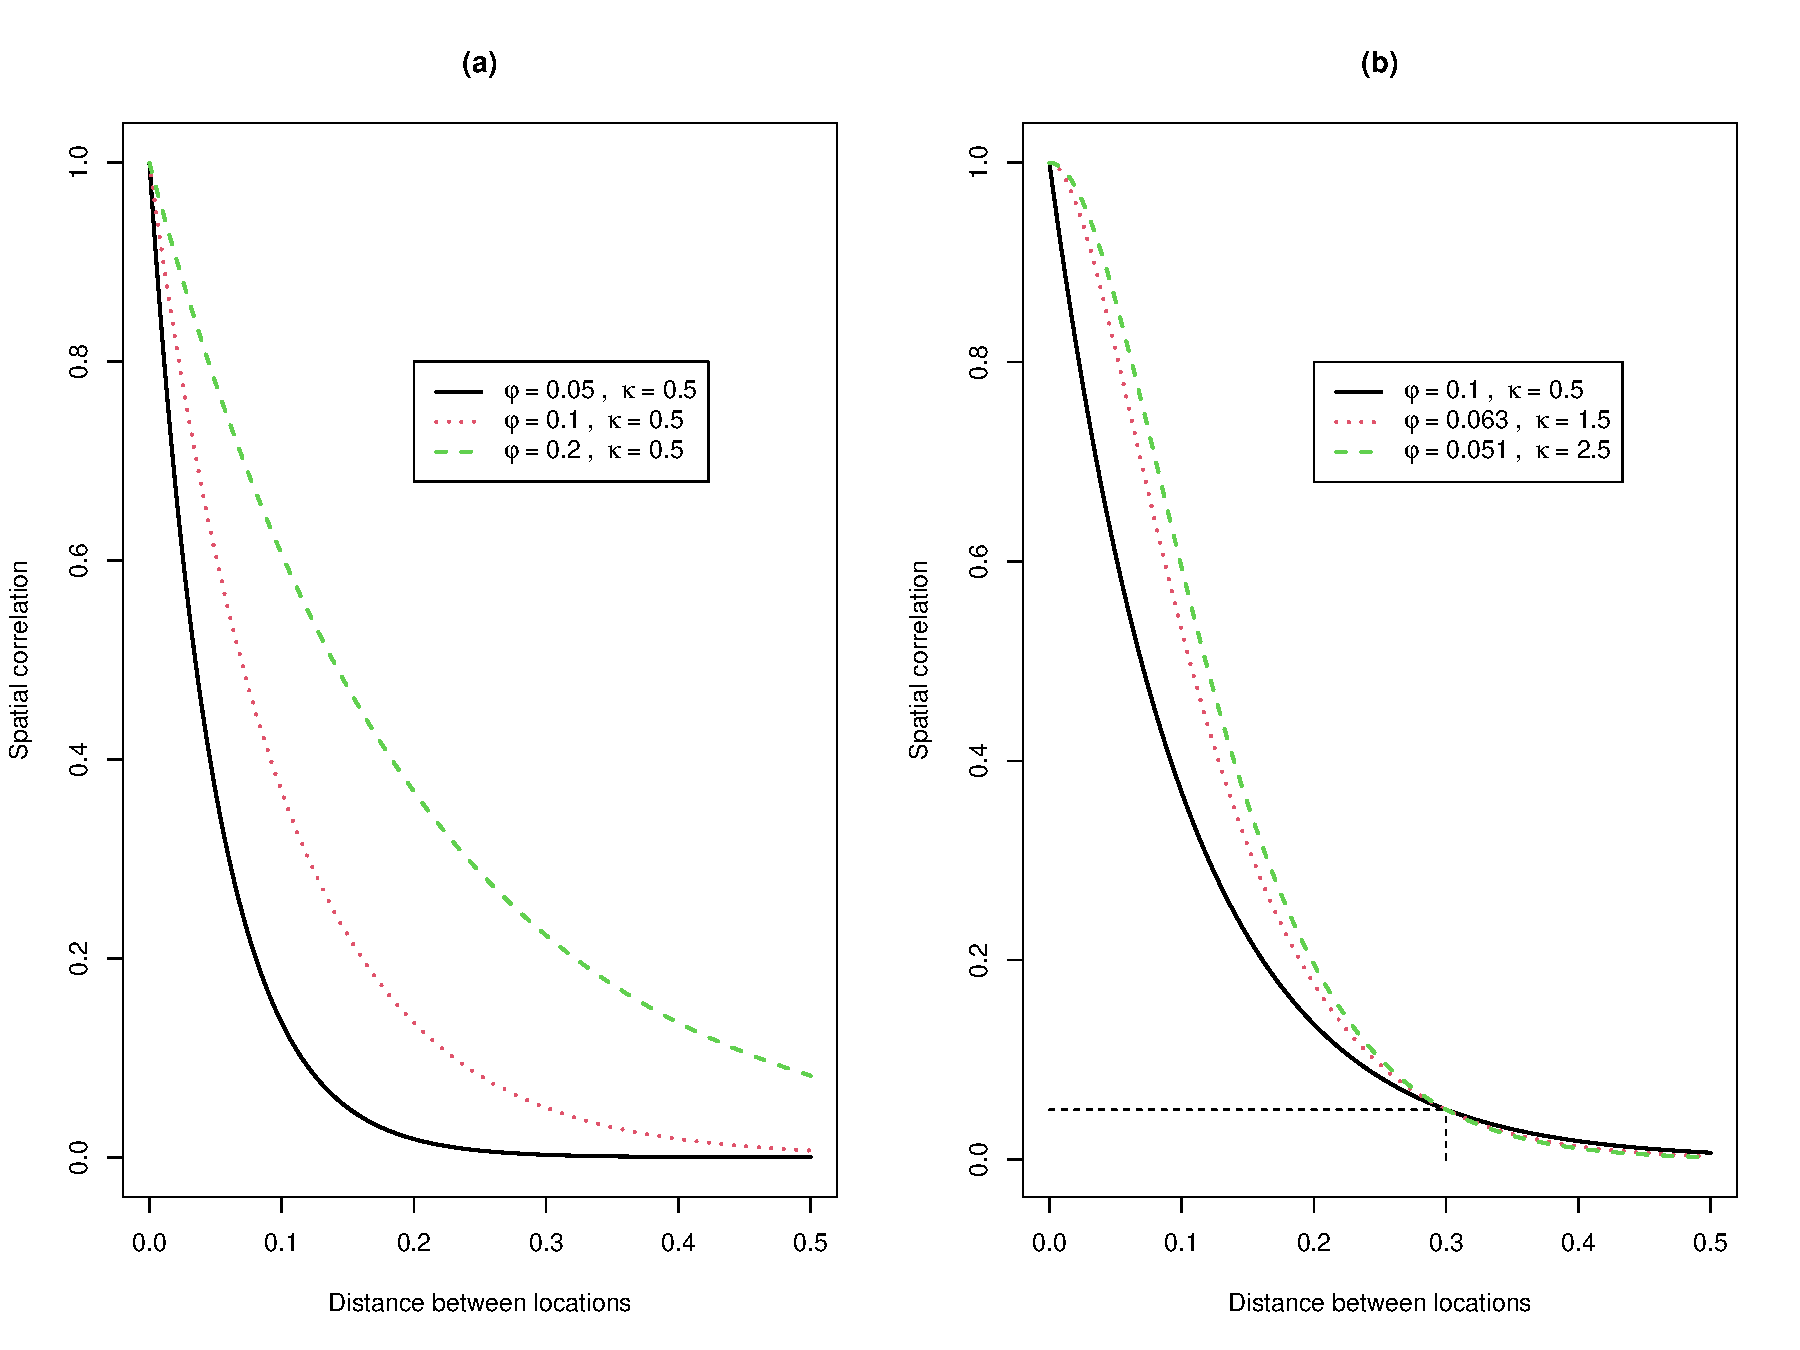
\includegraphics[width=8.5in,height=\textheight]{01_intro_files/figure-pdf/fig-matern-func-1.pdf}

}

\caption{\label{fig-matern-func}Examples of stationary and isotropic
Matern correlation functions. Panel (a) shows three different
correlations functions that have the same smothness parameter of
\(\kappa=0.5\), while varying the scale parameter \(\phi\) over
\({0.05, 0.1, 0.2}\). In panel (b) the scale of the spatial correlation
\(\phi\) is chosen so that each of the three functions reaches 0.05 at
distance 0.3 (as also shown by the horizontal and vertical black dashed
segments).}

\end{figure}

Figure~\ref{fig-matern-func} shows six different Matern correlation
functions. In panel (a), we have kept \(\kappa\) fixed to 0.5 and varied
\(\phi\) over the values 0.05, 0.1 and 0.2. As expected, for larger
values of \(\phi\) the correlation function has a slower decay to zero.
Panels (a) to (c), in Figure~\ref{fig-matern-sim}, show three
realizations of a Gaussian process from each of these correlation
functions. The mean of the Gaussian process was set to zero and variance
to 1. We can observe that spatial correlations with larger scales are
associated with longer spatial trends, whilst smaller scales exhibit a
patchier pattern. This is because, as \(\phi\) takes values that are
closer to zero, the spatial surface will tend to show a less structured
pattern and will revert towards its zero mean more rapidly.

Finally, let us consider the correlation functions, shown in the panel
(b) of Figure~\ref{fig-matern-func}. Here, we have varied \(\kappa\)
over the values 0.5, 1.5 and 2.5, whilst \(\phi\) has been fixed in
order to force all three correlation functions to reach 0.05 for
distance 0.3. In this way, we can better observe the effect of different
values \(\kappa\) on the spatial surface for process that have
approximately the same range for the spatial correlation. In
Figure~\ref{fig-matern-sim}, we observe three realizations from these
correlation functions. We observe that the differences between the
different surface are determined by the small spatial scale behaviour;
\(\kappa = 0.5\) correspond to a rougher and less regular spatial
pattern, whilst \(\kappa=2.5\) shows a smoothest surface of the three
processes considered. These properties of the spatial surface are
related to the so called differentiability of the the Guassian process,
which determines its local behaviour. If you are interested in delving
these theoretical aspects, we suggest reading Chapter 2 of Stein (1999).

\begin{figure}

{\centering 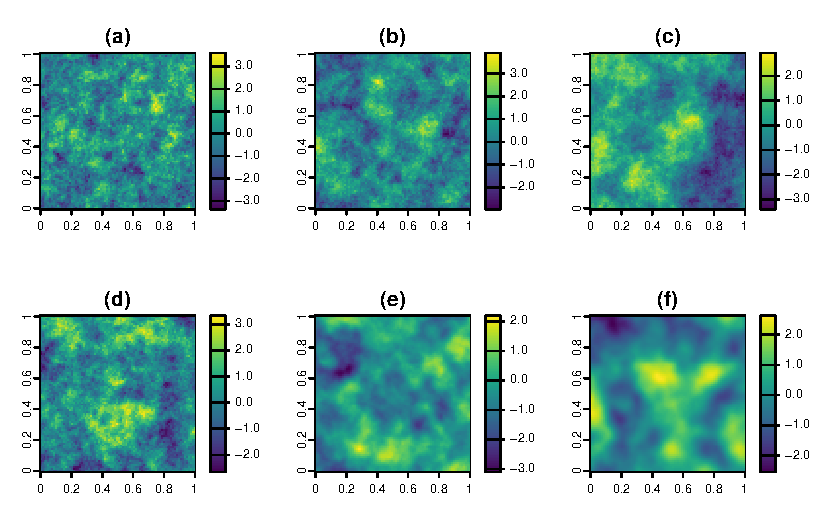
\includegraphics{01_intro_files/figure-pdf/fig-matern-sim-1.pdf}

}

\caption{\label{fig-matern-sim}Simulated spatial surface using the three
correltion functions shown in Figure~\ref{fig-matern-func}. Panels (a),
(b) and (c) correspond to the correlation functions from panel (a) in
Figure~\ref{fig-matern-func} and in order these are: \(\phi = 0.05\) and
\(\kappa=0.5\); (b) \(\phi=0.1\) and \(\kappa=0.5\); (c) \(\phi=0.2\)
and \(\kappa=0.5\). Panels (c), (d) and (e) correspond to the
correlation functions from panel (b) in Figure~\ref{fig-matern-func} and
in order these are: \(\phi = 0.1\) and \(\kappa=0.5\); (b)
\(\phi=0.063\) and \(\kappa=1.5\); (c) \(\phi=0.051\) and
\(\kappa=2.5\).}

\end{figure}

The flexibility provided by the Matern correlation function in capturing
different forms of spatial correlations has made one of, if not the most
widely used correlation function in model-based geostatistics (Stein
1999). For this reason, in this book we will consider the Matern
correlation function. We will consider estimation issues related to the
Matern correlation in Chapter~\ref{sec-estimation}.

\hypertarget{workflow-of-a-statistical-analysis-and-structure-of-the-book}{%
\section{Workflow of a statistical analysis and structure of the
book}\label{workflow-of-a-statistical-analysis-and-structure-of-the-book}}

\begin{figure}

{\centering 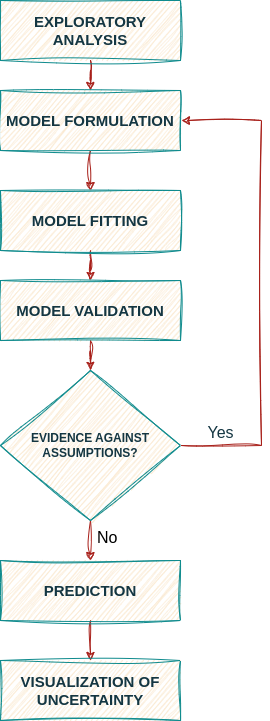
\includegraphics{./figures/workflow_diagram.png}

}

\caption{\label{fig-stages}Stages of a statistical analysis}

\end{figure}

Figure~\ref{fig-stages} shows the different stages that will follow in
carrying the geostatistical analysis of the examples introduced in
Section~\ref{sec-examples-ch1}. The exploratory analysis of the data is
an essential first step that is used to understand the empirical
associations between risk factors and the the health outcome of
interest. In our case, this first stage is also used to justify the use
of geostatistical models by questioning the underlying assumptions of
standard generalized linear models. Based on the results obtained from
the exploration of the data, we then formulate a suitable statistical
model and estimate its parameters using likelihood based methods of
inference. These also allows us to obtain uncertainty measures about the
strength of associations of regression relationships and the other model
parameters that define the shape of the spatial correlation in the data.
Following the estimation of the model, we then proceed to validate its
underlying assumptions using suitable diagnostics that assess whether
the model can later be sufficiently trusted to represent the observed
variation in the modelled outcome. At this stage, if the diagnostics
checks yield results that indicate the incompatibility of the model with
the data, we then back to the stage of model formulation and address the
issues arisen from the validation stage. If instead, we do not find any
evidence against the fitted model we can proceed to carry out sptatial
prediction. At this stage, it is important to define suitable predictive
targets that can help us to better answer the original research question
and better assist the decision making process. The final step of
visualization of uncertainty plays an important role in geostatistical
analysis in order to convey the main findings of the study in an
effective and easy-to-understand way for a wider audience which also
consists of non-experts.

In the remainder of this book, each chapter focuses on a specific stage
as shown in Figure~\ref{fig-stages}. We treat visualization of
uncertainty together with spatial prediction in
Chapter~\ref{sec-geo-prediction}.

Chapter~\ref{sec-handling-data} will provide an overview of how to
handle saptial data in R, in particular raster and shape files. The
skills learned in this chapter will be applied throughout the book, and
will especially be useful in Chapter~\ref{sec-geo-prediction} and
Chapter~\ref{sec-case-studies} for generating predictive maps of the
modelled outcome.

Chapter~\ref{sec-estimation} focuses on the model building process and
estimation of geostatistical models. This chapter will show how to carry
out initial exploratory analyses of the data to inform the formulation
of suitable geostatistical models and how these can be fitted using
maximum likelihood estimation methods.

Chapter~\ref{sec-validation} illustrated the use of methods that can be
used to validate the assumptions and calibration of statistical models.

Chapter~\ref{sec-geo-prediction} shows how geostatistical models can be
used to carry out spatial prediction of a health outcome of interest
both on a spatially continuous and spatially aggregated scales.

Finally, Chapter~\ref{sec-case-studies} presents the application of all
the methods illustrated in the previous chapters to three additional
data-sets. This chapter offers a summary of the content of book by
putting together all the stages in the geostatistical analyses for each
of the three case studies, and illustrates additional functionalities of
the \texttt{RiskMap} R package not covered in the previous chapters.

\bookmarksetup{startatroot}

\hypertarget{sec-handling-data}{%
\chapter{Handling of spatial data in R}\label{sec-handling-data}}

This is a book created from markdown and executable code.

See (\textbf{knuth84?}) for additional discussion of literate
programming.

\begin{Shaded}
\begin{Highlighting}[]
\DecValTok{1} \SpecialCharTok{+} \DecValTok{1}
\end{Highlighting}
\end{Shaded}

\begin{verbatim}
[1] 2
\end{verbatim}

\hypertarget{importing-and-processing-spatial-data-in-r}{%
\section{Importing and processing spatial data in
R}\label{importing-and-processing-spatial-data-in-r}}

\hypertarget{visualizing-geostatistical-data}{%
\section{Visualizing geostatistical
data}\label{visualizing-geostatistical-data}}

\hypertarget{section}{%
\section{}\label{section}}

\bookmarksetup{startatroot}

\hypertarget{sec-estimation}{%
\chapter{Model formulation and parameter
estimation}\label{sec-estimation}}

\hypertarget{list-of-the-main-functions-used-in-the-chapter}{%
\section*{List of the main functions used in the
chapter}\label{list-of-the-main-functions-used-in-the-chapter}}
\addcontentsline{toc}{section}{List of the main functions used in the
chapter}

\markright{List of the main functions used in the chapter}

\begin{longtable}[]{@{}
  >{\raggedright\arraybackslash}p{(\columnwidth - 4\tabcolsep) * \real{0.2055}}
  >{\raggedright\arraybackslash}p{(\columnwidth - 4\tabcolsep) * \real{0.2055}}
  >{\raggedright\arraybackslash}p{(\columnwidth - 4\tabcolsep) * \real{0.5890}}@{}}
\toprule\noalign{}
\begin{minipage}[b]{\linewidth}\raggedright
Function
\end{minipage} & \begin{minipage}[b]{\linewidth}\raggedright
R Package
\end{minipage} & \begin{minipage}[b]{\linewidth}\raggedright
Used for
\end{minipage} \\
\midrule\noalign{}
\endhead
\bottomrule\noalign{}
\endlastfoot
\texttt{lmer} & \texttt{lme4} & Fitting linear mixed models \\
\texttt{glmer} & \texttt{lme4} & Fitting generalized linear mixed
models \\
\texttt{glgm} & \texttt{RiskMap} & Fitting generalized linear mixed
models \\
\texttt{s\_variogram} & \texttt{RiskMap} & Computing the empirical
variogram and carrying out permutation test for spatial independence \\
\end{longtable}

\hypertarget{exploratory-analysis}{%
\section{Exploratory analysis}\label{exploratory-analysis}}

As illustrated in Figure~\ref{fig-stages}, exploratory analysis is the
first step that should be carried out in a statistical analysis. This
stage is essential to inform how covariates should be introduced in the
model and, in our case, whether the variation unexplained by those
covariates exhibits spatial correlation.

In the exploratory analysis of count data, we will also look at how
overdispersion, which is a necessary, though not sufficient, condition
for residual spatial correlation.

\hypertarget{sec-expl-assoc}{%
\subsection{Exploring associations with risk factors using count
data}\label{sec-expl-assoc}}

Assessment of the association between the health outcome of interest and
non-categorical (i.e.~continuous) risk factors can be carried using
graphical tools, such scatter plots. The graphical inspection of the
empirical association between the outcome and the covariates is
especially useful to identify non-linear patterns in the relationship
which should then be accounted for in the model formulation.

In this section, we look more closely at the case when the observed
outcome is a count which requires a different treatment from
continuously measured outcomes, which are generally covered by most
statistics textbooks (see, for example, Chapter 1 of Weisberg (2014)).

\hypertarget{when-the-outcome-is-an-aggregated-count}{%
\subsubsection{When the outcome is an aggregated
count}\label{when-the-outcome-is-an-aggregated-count}}

Let us first consider the example of the river-blindness data in Liberia
(Section~\ref{sec-rb-ch1}), and examine the association between
prevalence and elevation. We first generate a plot of the prevalence
against the measured elevation at each of the sample locations

\begin{Shaded}
\begin{Highlighting}[]
\NormalTok{liberia}\SpecialCharTok{$}\NormalTok{prev }\OtherTok{\textless{}{-}}\NormalTok{ liberia}\SpecialCharTok{$}\NormalTok{npos}\SpecialCharTok{/}\NormalTok{liberia}\SpecialCharTok{$}\NormalTok{ntest}

\FunctionTok{ggplot}\NormalTok{(liberia, }\FunctionTok{aes}\NormalTok{(}\AttributeTok{x =}\NormalTok{ elevation, }\AttributeTok{y =}\NormalTok{ prev)) }\SpecialCharTok{+} \FunctionTok{geom\_point}\NormalTok{() }\SpecialCharTok{+}
  \FunctionTok{labs}\NormalTok{(}\AttributeTok{x=}\StringTok{"Elevation (meters)"}\NormalTok{,}\AttributeTok{y=}\StringTok{"Prevalence"}\NormalTok{)}
\end{Highlighting}
\end{Shaded}

\begin{figure}[H]

{\centering 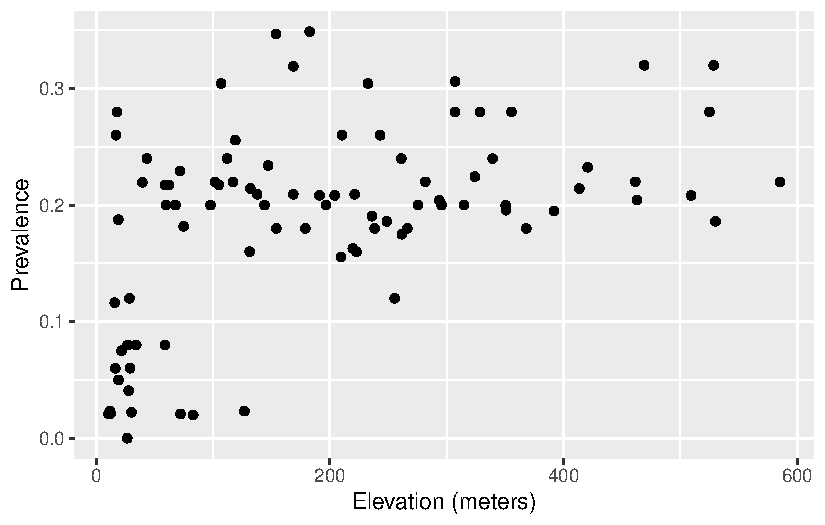
\includegraphics{03_model-fitting_files/figure-pdf/fig-prev-elev-liberia-1.pdf}

}

\caption{\label{fig-prev-elev-liberia}Scatter plot of the empirical
prevalence for river-blindess against elevation, measured in meters.}

\end{figure}

The plot shown in Figure~\ref{fig-prev-elev-liberia} shows that, as
elevation increases from 0 to around 150 meters, prevalence rapidly
increases to around 0.25 and, for larger values in elevation than 150
meters, the relationship levels off. This begs the question of how we
can account for this in a regression model. To answer this question
rigorously, however, the plot in Figure~\ref{fig-prev-elev-liberia}
cannot be used. This is because, when the modelled outcome is a bounded
Binomial count, regression relationships are specified on the
logit-transformed prevalence (log-odds) scale; see Table~\ref{tbl-glm}
in Section Section~\ref{sec-geostat-models} . To explore regression
relationships in the case of prevalence data, it is convenient to use
the so-called empirical logit in place of the empirical prevalence. The
empirical logit is defined as

\begin{equation}\protect\hypertarget{eq-empirical-logit}{}{
l_{i} = \log\left\{\frac{y_i + 1/2}{n_i - y_i + 1/2}\right\}
}\label{eq-empirical-logit}\end{equation}

where \(y_i\) are the number of individuals who tested positive for
riverblindness and \(n_i\) is the total number of people tested at a
location. The reason for using the empirical logit, rather than the
standard logit transformation applied directly to the empirical
prevalence, is that it allows to generate finite values for empirical
prevalence values of 0 and 1, for which the standard logit
transformation is not defined.

\begin{Shaded}
\begin{Highlighting}[]
\CommentTok{\# The empirical logit}
\NormalTok{liberia}\SpecialCharTok{$}\NormalTok{elogit }\OtherTok{\textless{}{-}} \FunctionTok{log}\NormalTok{((liberia}\SpecialCharTok{$}\NormalTok{npos}\FloatTok{+0.5}\NormalTok{)}\SpecialCharTok{/}
\NormalTok{                      (liberia}\SpecialCharTok{$}\NormalTok{ntest}\SpecialCharTok{{-}}\NormalTok{liberia}\SpecialCharTok{$}\NormalTok{npos}\FloatTok{+0.5}\NormalTok{))}

\FunctionTok{ggplot}\NormalTok{(liberia, }\FunctionTok{aes}\NormalTok{(}\AttributeTok{x =}\NormalTok{ elevation, }\AttributeTok{y =}\NormalTok{ elogit)) }\SpecialCharTok{+} \FunctionTok{geom\_point}\NormalTok{() }\SpecialCharTok{+}
  
  \CommentTok{\# Adding a smoothing spline}
  \FunctionTok{labs}\NormalTok{(}\AttributeTok{x=}\StringTok{"Elevation (meters)"}\NormalTok{,}\AttributeTok{y=}\StringTok{"Empirical logit"}\NormalTok{) }\SpecialCharTok{+}
  \FunctionTok{stat\_smooth}\NormalTok{(}\AttributeTok{method =} \StringTok{"gam"}\NormalTok{, }\AttributeTok{formula =}\NormalTok{ y }\SpecialCharTok{\textasciitilde{}} \FunctionTok{s}\NormalTok{(x),}\AttributeTok{se=}\ConstantTok{FALSE}\NormalTok{)}\SpecialCharTok{+}
  
  \CommentTok{\# Adding linear regression fit with log{-}transformed elevation}
  \FunctionTok{stat\_smooth}\NormalTok{(}\AttributeTok{method =} \StringTok{"lm"}\NormalTok{, }\AttributeTok{formula =}\NormalTok{ y }\SpecialCharTok{\textasciitilde{}} \FunctionTok{log}\NormalTok{(x),}
              \AttributeTok{col=}\StringTok{"green"}\NormalTok{,}\AttributeTok{lty=}\StringTok{"dashed"}\NormalTok{,}\AttributeTok{se=}\ConstantTok{FALSE}\NormalTok{) }\SpecialCharTok{+}

  \CommentTok{\# Adding linear regression fit with change point in 150 meters}
  \FunctionTok{stat\_smooth}\NormalTok{(}\AttributeTok{method =} \StringTok{"lm"}\NormalTok{, }\AttributeTok{formula =}\NormalTok{ y }\SpecialCharTok{\textasciitilde{}}\NormalTok{ x }\SpecialCharTok{+} \FunctionTok{pmax}\NormalTok{(x}\DecValTok{{-}150}\NormalTok{, }\DecValTok{0}\NormalTok{),}
              \AttributeTok{col=}\StringTok{"red"}\NormalTok{,}\AttributeTok{lty=}\StringTok{"dashed"}\NormalTok{,}\AttributeTok{se=}\ConstantTok{FALSE}\NormalTok{) }
  
\end{Highlighting}
\end{Shaded}

\begin{figure}[H]

{\centering 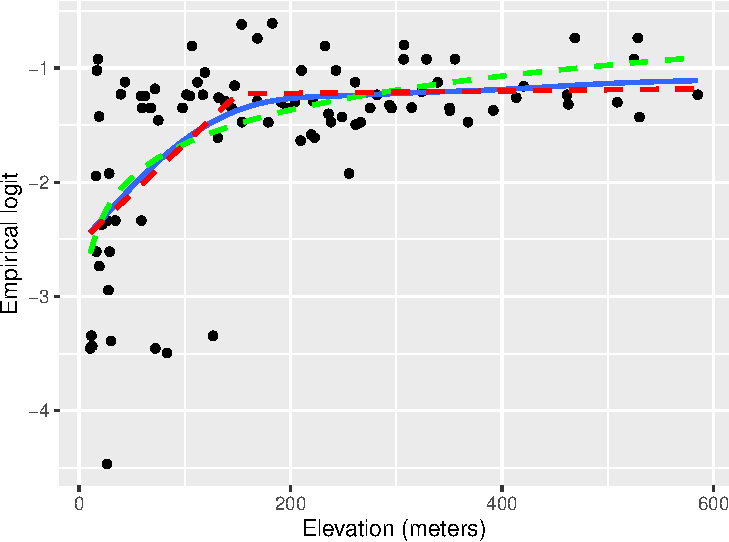
\includegraphics{03_model-fitting_files/figure-pdf/fig-elogit-elev-liberia-1.pdf}

}

\caption{\label{fig-elogit-elev-liberia}Scatter plot of the empirical
prevalence for river-blindess against elevation, measured in meters.}

\end{figure}

Figure~\ref{fig-elogit-elev-liberia} shows the scatter plot of the
empirical logit against elevation. In this plot, we have also added
three lines though the \texttt{stat\_smooth} from the \texttt{ggplot2}
package. Using this function, we first pass the term \texttt{gam} to
\texttt{method} to add a penalized smoothing spline (Hastie, Tibshirani,
and Friedman 2001), represented by the blue solid line. The smoothing
spline allows us to better discern how the type of relationship and how
to best capture it using a standard regression approach. As er can see
from Figure~\ref{fig-elogit-elev-liberia}, the smoothing spline
corroborates our initial observation of a positive relationship up to
about 150 meters, followed by a plateau.

To capture this non-linear relationship, we can use the two following
approaches. The first is based on a simple log-transformation of
elevation and is represented in Figure~\ref{fig-elogit-elev-liberia} by
the green line. If were to express this relationship using a standard
Binomial regression model, this would take the form
\begin{equation}\protect\hypertarget{eq-log-elev-glm}{}{
\log\left\{\frac{p(x_i)}{1-p(x_i)}\right\} = \beta_0 + \beta_1 \log\{e(x_i)\}
}\label{eq-log-elev-glm}\end{equation} where \(p(x_i)\) and \(e(x_i)\)
are the river-blindness prevalence and elevation at sampled location
\(x_i\), respectively.

Alternatively, the non-linear effect of elevation on prevalence could be
captured using a linear spline. Put in simple terms, we want to fit a
linear regression model that allows for a change in slope above 150
meters. Formally, this is expressed in a Binomial regression model as
\begin{equation}\protect\hypertarget{eq-lspline-elev-glm}{}{
\log\left\{\frac{p(x_i)}{1-p(x_i)}\right\} = \beta_0 + \beta_1 e(x_i) + \beta_{2} \max\{e(x_i)-150, 0\}.
}\label{eq-lspline-elev-glm}\end{equation} Based on the equation above,
the effect of elevation below 150 meters is quantified by the parameter
\(\beta_1\). Above 150 meters, instead, the effect of elevation becomes
\(\beta_1 + \beta_2\). Note that the function \texttt{pmax} (and not the
standard base function \texttt{max}) should be used in R when the
computation of the maximum between a scalar value and each of the
components of a numeric vector is required.

Before proceeding further, it is important to explain the differences
between the use of the logarithmic transformation
(Equation~\ref{eq-log-elev-glm}) and the linear spline
(Equation~\ref{eq-lspline-elev-glm}). We observe that both curves
provide a similar fit to the data, with larger differences observed for
larger values in elevation, where the log-transformed elevation models
yields larger values for the predicted prevalence. This also suggests
that if we were to extrapolate the predictions beyond 600 meters in
elevation the implied pattern by the model with the log-transformed
elevation would predict an increasingly larger elevation, which is
unrealistic, since the fly that transmits the diseases cannot breed at
those altitudes. The linear spline model instead would generate
predictions that would be very similar to those observed between 150 and
600 meters. From this point view, the linear spline model would thus
have more scientific validity than the other model. However, which of
the two approaches should be chosen to model the effect of elevation is
a question that closely depends on the research question to be
addressed.

If the interest of the study was in better understanding the association
between elevation and prevalence, the linear spline model does not only
provide a more credible explanation but also its regression parameters
can be more easily interpreted. In fact, for a unit increase in
elevation, the multiplicative change in the odds for river-blindness is
\(\exp\{\beta_1\}\), if elevation is below 150 meters, and
\(\exp\{\beta_1+\beta_2\}\), if elevation is above 150 meters. When
instead we use the log-transformed elevation, the interpretation of
\(\beta_1\) in Equation~\ref{eq-log-elev-glm} is slightly more
complicated, as it is based on the multiplicative increase in elevation
by the same amount given by the base of the algorithm, which is about
\(e \approx 2.718\)\footnote{The letter \(e\) stands for the so called
  Euler's number and represents the base of the natural logarithm. In
  the book, we write \(\log(\cdot)\) to mean the ``natural logarithm of
  \(\cdot\)''.}. To avoid this, one could rescale the regression
coefficient as, for example, \(\beta_1/\log_{2}(e)\) which would be
interpreted as the multiplicative change in the odds for river-blindness
for a doubling in elevation. However, a doubling in elevation is less
meaningful when considering larger values of elevation.

When the goal of statistical analysis is instead in developing a
predictive model for the outcome of interest, the explanatory power and
interpretability of the model may be of less concern. For this reason,
the model with the log-transformed model could be preferred over the
model with the linear spline, if it shown to yield more predictive
power. We will come back to this point again in
Chapter~\ref{sec-geo-prediction}, where will show how to assess and
compare the predictive performance of different geostatistical models.

The other type of aggregated count data that we consider are unbounded
counts. The Anopheles mosquitoes data-set
(Section~\ref{sec-mosq-data-ch1}) is an example of this, since there is
no upper limit to the number of mosquitoes that can be trapped at a
location. Let us consider the covariate represented by elevation. In
this case, the simplest model that can be used to analyse the data is a
Poisson regression, where the linear predictor is defined on the log of
the mean number of mosquitoes (Table~\ref{tbl-glm}). Hence, exploratory
plots for the association with covariates should be generated using the
log transformed counts of mosquitoes. In this instance, to avoid taking
the log of zero, we can add 1 to the reported counts, if required. The
variable of the \texttt{An.gambiae} in the \texttt{anopheles} data-set
does not contain any 0, hence we simply apply the log tranformation
without adding 1.

\begin{Shaded}
\begin{Highlighting}[]
\NormalTok{anopheles}\SpecialCharTok{$}\NormalTok{log\_counts }\OtherTok{\textless{}{-}} \FunctionTok{log}\NormalTok{(anopheles}\SpecialCharTok{$}\NormalTok{An.gambiae)}
\FunctionTok{ggplot}\NormalTok{(anopheles, }\FunctionTok{aes}\NormalTok{(}\AttributeTok{x =}\NormalTok{ elevation, }\AttributeTok{y =}\NormalTok{ log\_counts)) }\SpecialCharTok{+} \FunctionTok{geom\_point}\NormalTok{() }\SpecialCharTok{+}
  
  \CommentTok{\# Adding a smoothing spline}
  \FunctionTok{labs}\NormalTok{(}\AttributeTok{x=}\StringTok{"Elevation (meters)"}\NormalTok{,}\AttributeTok{y=}\StringTok{"Log number of An. gambiae mosquitoes"}\NormalTok{) }\SpecialCharTok{+}
  \FunctionTok{stat\_smooth}\NormalTok{(}\AttributeTok{method =} \StringTok{"lm"}\NormalTok{, }\AttributeTok{formula =}\NormalTok{ y }\SpecialCharTok{\textasciitilde{}}\NormalTok{ x, }\AttributeTok{se=}\ConstantTok{FALSE}\NormalTok{)}
\end{Highlighting}
\end{Shaded}

\begin{figure}[H]

{\centering 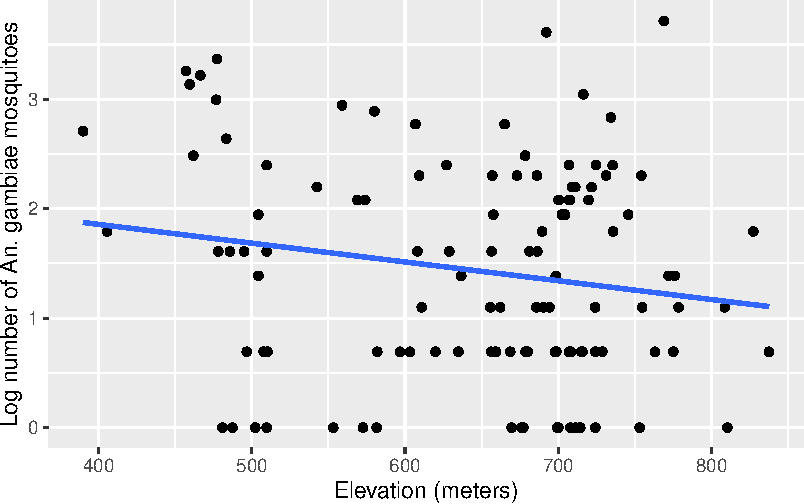
\includegraphics{03_model-fitting_files/figure-pdf/fig-logcounts-elev-mosq-1.pdf}

}

\caption{\label{fig-logcounts-elev-mosq}Scatter plot of the log
tranformed number of \emph{Anopheles gambiae} mosquitoes against
elevation, measured in meters. The blue line is generated using the
least squares fit.}

\end{figure}

The scatter plot of Figure~\ref{fig-logcounts-elev-mosq} shows that
there is a negative, though weak, association, with the average number
of mosquitoes decreasing for increasing elevation. In this instance, the
assumption of a linear relationship with elevation would be a reasonable
choice.

\hypertarget{when-the-outcome-is-an-invidual-level-binary-indicator}{%
\subsubsection{When the outcome is an invidual-level binary
indicator}\label{when-the-outcome-is-an-invidual-level-binary-indicator}}

We now consider the malaria data from Kenya
(Section~\ref{sec-malaria-ch1}) where the main outcome is the result
from a rapid diagnostic test (RDT) for malaria from individuals within
households. In this case, because the outcome only takes two values, 1
for a positive RDT test result and 0 otherwise, the direct application
of the empirical logit from Equation~\ref{eq-empirical-logit} would not
help us to generate informative scatter plots. Throughout the book, we
will consider the data from the community survey only, hence we work
with a subset of the data which we shall name \texttt{malkenya\_comm}

\begin{Shaded}
\begin{Highlighting}[]
\NormalTok{malkenya\_comm }\OtherTok{\textless{}{-}}\NormalTok{ malkenya[malkenya}\SpecialCharTok{$}\NormalTok{Survey}\SpecialCharTok{==}\StringTok{"community"}\NormalTok{, ]}
\end{Highlighting}
\end{Shaded}

To show how this issue can be overcome, let us consider the variables
age and gender. To generate a plot that can help us understand between
the relationship with malaria prevalence and the two risk factors, we
proceed as follows.

\begin{Shaded}
\begin{Highlighting}[]
\CommentTok{\# Grouping of ages into classes defined through "breaks"}
\NormalTok{malkenya\_comm}\SpecialCharTok{$}\NormalTok{Age\_class }\OtherTok{\textless{}{-}} \FunctionTok{cut}\NormalTok{(malkenya\_comm}\SpecialCharTok{$}\NormalTok{Age, }
                            \AttributeTok{breaks =} \FunctionTok{c}\NormalTok{(}\DecValTok{0}\NormalTok{, }\DecValTok{5}\NormalTok{, }\DecValTok{10}\NormalTok{, }\DecValTok{15}\NormalTok{, }\DecValTok{30}\NormalTok{, }\DecValTok{40}\NormalTok{, }\DecValTok{50}\NormalTok{, }\DecValTok{100}\NormalTok{),}
                            \AttributeTok{include.lowest =} \ConstantTok{TRUE}\NormalTok{)}
\end{Highlighting}
\end{Shaded}

Using the \texttt{cut} function, we first split age (in years) into
classes through the argument \texttt{breaks}. The classification of age
into \([0,5]\), \((5, 10]\) and \((10, 15]\) is common in many malaria
epidemiology studies, as children are one of the groups at highest risk
malaria. The choice of the other classes of age reflects instead the
need to balance the number of observations falling in each of the
classes.

\begin{Shaded}
\begin{Highlighting}[]
\CommentTok{\# Computation of the empirical logit by age groups and gender}
\NormalTok{age\_class\_data }\OtherTok{\textless{}{-}} \FunctionTok{aggregate}\NormalTok{(RDT }\SpecialCharTok{\textasciitilde{}}\NormalTok{ Age\_class }\SpecialCharTok{+}\NormalTok{ Gender, }
                                    \AttributeTok{data =}\NormalTok{ malkenya\_comm, }
                                    \AttributeTok{FUN =} \ControlFlowTok{function}\NormalTok{(y) }
                                    \FunctionTok{log}\NormalTok{((}\FunctionTok{sum}\NormalTok{(y)}\SpecialCharTok{+}\FloatTok{0.5}\NormalTok{)}\SpecialCharTok{/}\NormalTok{(}\FunctionTok{length}\NormalTok{(y)}\SpecialCharTok{{-}}\FunctionTok{sum}\NormalTok{(y)}\SpecialCharTok{+}\FloatTok{0.5}\NormalTok{)))}
\end{Highlighting}
\end{Shaded}

We then compute the empirical logit, using the total number of cases
within age group and by gender. For a given age group and gender, which
we denote as \(\mathcal{C}\), the empirical logit in
Equation~\ref{eq-empirical-logit}, now takes the form
\begin{equation}\protect\hypertarget{eq-empirical-logit-bin}{}{
l_{\mathcal{C}} = \log\left\{\frac{\sum_{i \in \mathcal{C}} y_{i} + 0.5}{|\mathcal{C}|- \sum_{i \in \mathcal{C}} y_{i} + 0.5} \right\}
}\label{eq-empirical-logit-bin}\end{equation} where \(y_i\) are the
individual binary outcomes and \(i\in \mathcal{C}\) is used to indicate
that the sum is carried out over all the individuals who belong the
class \(\mathcal{C}\), identified by a specific age group and gender.
Finally, \(|\mathcal{C}|\) is the number of individuals who fall within
\(\mathcal{C}\). In the code above, the empirical logit in
Equation~\ref{eq-empirical-logit-bin} is computed using the
\texttt{aggregate} function. An inspection of the object
\texttt{age\_class\_data}, a data frame, shows that the empirical is
found in the column named \texttt{RDT}.

\begin{Shaded}
\begin{Highlighting}[]
\CommentTok{\# Computation of the average age within each age group }
\NormalTok{age\_class\_data}\SpecialCharTok{$}\NormalTok{age\_mean\_point }\OtherTok{\textless{}{-}} \FunctionTok{aggregate}\NormalTok{(Age }\SpecialCharTok{\textasciitilde{}}\NormalTok{ Age\_class }\SpecialCharTok{+}\NormalTok{ Gender, }
                                 \AttributeTok{data =}\NormalTok{ malkenya\_comm, }
                                 \AttributeTok{FUN =}\NormalTok{ mean)}\SpecialCharTok{$}\NormalTok{Age}


\CommentTok{\# Number of individuals within each age group, by gender}
\NormalTok{age\_class\_data}\SpecialCharTok{$}\NormalTok{n\_obs }\OtherTok{\textless{}{-}}  \FunctionTok{aggregate}\NormalTok{(Age }\SpecialCharTok{\textasciitilde{}}\NormalTok{ Age\_class }\SpecialCharTok{+}\NormalTok{ Gender, }
                         \AttributeTok{data =}\NormalTok{ malkenya\_comm, }
                         \AttributeTok{FUN =}\NormalTok{ length)}\SpecialCharTok{$}\NormalTok{Age}
\end{Highlighting}
\end{Shaded}

In order to generate the scatter-plot, we compute the average age within
each age group by gender, and use these as our values for the x-axis.
Note that since we only need to obtain the average age from this output,
we use \texttt{\$Age} to extract this only and allocate to the column
\texttt{age\_mean\_point}. Finally, we also compute the number of
observations within each of classes and place this in \texttt{n\_obs}.

\begin{Shaded}
\begin{Highlighting}[]
\FunctionTok{ggplot}\NormalTok{(age\_class\_data, }\FunctionTok{aes}\NormalTok{(}\AttributeTok{x =}\NormalTok{ age\_mean\_point, }\AttributeTok{y =}\NormalTok{ RDT, }
                           \AttributeTok{size =}\NormalTok{ n\_obs, }
                           \AttributeTok{colour =}\NormalTok{ Gender)) }\SpecialCharTok{+} 
  \FunctionTok{geom\_point}\NormalTok{() }\SpecialCharTok{+} 
  \FunctionTok{labs}\NormalTok{(}\AttributeTok{x=}\StringTok{"Age (years)"}\NormalTok{,}\AttributeTok{y=}\StringTok{"Empirical logit"}\NormalTok{)  }
\end{Highlighting}
\end{Shaded}

\begin{figure}[H]

{\centering 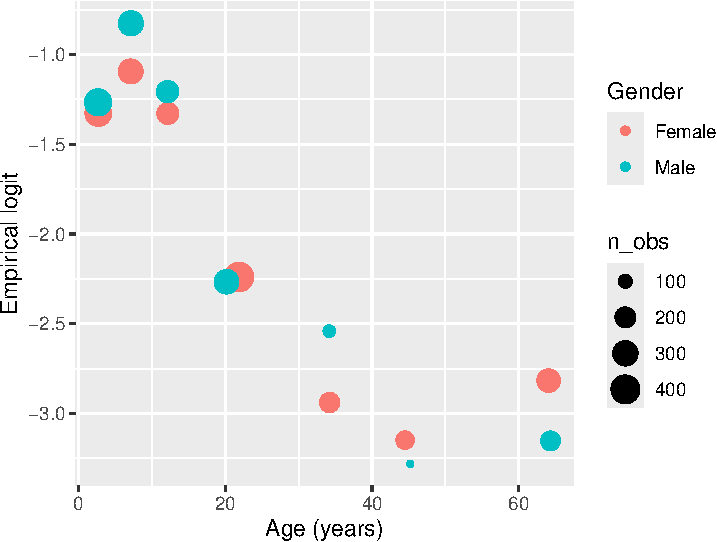
\includegraphics{03_model-fitting_files/figure-pdf/fig-elogit-age-malkenya-1.pdf}

}

\caption{\label{fig-elogit-age-malkenya}Plot of the empirical logit
against age, for males and females. The size of each solid point is
rendered proportional to the number of individuals within age group, as
indicated in the legend.}

\end{figure}

The resulting plot in Figure~\ref{fig-elogit-age-malkenya} shows the
empirical logit against age by gender, with the size of each of the
points proportional to the number of observations falling within each
class. The observed patterns are explained by the fact that young
children, especially those under the age of five, are particularly
vulnerable to severe malaria infections. This is primarily due to their
immature immune systems and lack of acquired immunity. As individuals
grow older, they generally develop partial immunity to malaria through
repeated exposure to the disease. This acquired immunity can provide
some level of protection against severe malaria. At the same time,
gender roles and activities can influence exposure to malaria-carrying
mosquitoes. For example, men may spend more time outdoors for work or
other activities, increasing their exposure to mosquito bites and thus
their risk of infection. In addition, there are also biological factors
to consider. Hormonal and genetic differences between males and females
may also contribute to variations in immune responses to malaria
infection. The interaction between age and gender is complex and may
vary depending on the specific context and population being studied. A
2020 report from the Bill \& Melinda Gates foundation provides a
detailed overview of this and other aspects related to gender and
malaria (Katz and Bill \& Melinda Gates Foundation 2020).

To account for age in a model for malaria prevalence, several approaches
are possible, some of which have been developed using biological models
(Smith et al. 2007). To model the patterns observed in
Figure~\ref{fig-elogit-age-malkenya}, we can follow the same approach
used in the previous section to model the relationship between elevation
and river-blindness prevalence. First, let us consider age without the
effect of gender. Let \(p_{j}(x_i)\) denote the probability of a
positive RDT for the \(j\)-th individual living in a household at
location \(x_i\). Assuming that malaria risk reaches its peak at 15
years of age, we can capture the non-linear relationship using a linear
spline with two knots, one at 15 years and a second one at 40 years.
This is expressed as
\begin{equation}\protect\hypertarget{eq-age-only-reg}{}{
\begin{aligned}
\log\left\{\frac{p_{j}(x_i)}{1-p_j(x_i)}\right\} = \beta_{0} + \beta_{1}a_{ij}+\beta_{2} \times\max\{a_{ij}-15, 0\} + \beta_{3}\max\{a_{ij}-40, 0\}
\end{aligned}
}\label{eq-age-only-reg}\end{equation} where \(a_{ij}\) is the age, in
years, for the \(j\)-th individual at household \(i\). Based on this
model the effect of age on RDT prevalence is \(\beta_{1}\), for
\(a_{ij} < 15\), \(\beta_{1}+\beta_{2}\), for \(15 < a_{ij} < 40\), and
\(\beta_{1}+\beta_{2}+\beta_{3}\) for \(a_{ij} > 40\).

Figure~\ref{fig-elogit-age-malkenya} indicates that age may interact
with gender, meaning that the effect of gender on RDT prevalence changes
across age, with larger differences observed between males and females
for ages above 20 years. To assess such differences using a standard
Binomial regression model, the linear predictor for RDT prevalence can
be formulated as
\begin{equation}\protect\hypertarget{eq-age-inter-reg}{}{
\begin{aligned}
\log\left\{\frac{p_{j}(x_i)}{1-p_j(x_i)}\right\} = \beta_{0} + (\beta_{1} + \beta_{1}^*g_{ij})\times a_{ij}+(\beta_{2} + \beta_{2}^*g_{ij})\times\max\{a_{ij}-15, 0\} + \\
(\beta_{3} + \beta_{3}^*g_{ij}) \times \max\{a_{ij}-40, 0\}
\end{aligned}
}\label{eq-age-inter-reg}\end{equation} where \(g_{ij}\) is the
indicator for gender, with 1 corresponding to male and 0 to female. The
coefficients \(\beta_{1}^*\), \(\beta_{2}^*\) and \(\beta_{3}^*\) thus
quantify the differences in risk between the two genders for ages below
15 years, betwee 15 and 40 years, and above 40 years, respectively. If
all of those coefficients were 0, the model in
Equation~\ref{eq-age-only-reg} would be recovered.

\begin{Shaded}
\begin{Highlighting}[]
\NormalTok{glm\_age\_gender\_interaction }\OtherTok{\textless{}{-}} \FunctionTok{glm}\NormalTok{(RDT }\SpecialCharTok{\textasciitilde{}}\NormalTok{ Age }\SpecialCharTok{+}\NormalTok{ Gender}\SpecialCharTok{:}\NormalTok{Age }\SpecialCharTok{+} 
                                  \FunctionTok{pmax}\NormalTok{(Age}\DecValTok{{-}15}\NormalTok{, }\DecValTok{0}\NormalTok{) }\SpecialCharTok{+}\NormalTok{ Gender}\SpecialCharTok{:}\FunctionTok{pmax}\NormalTok{(Age}\DecValTok{{-}15}\NormalTok{, }\DecValTok{0}\NormalTok{) }\SpecialCharTok{+} 
                                  \FunctionTok{pmax}\NormalTok{(Age}\DecValTok{{-}40}\NormalTok{, }\DecValTok{0}\NormalTok{) }\SpecialCharTok{+}\NormalTok{ Gender}\SpecialCharTok{:}\FunctionTok{pmax}\NormalTok{(Age}\DecValTok{{-}40}\NormalTok{, }\DecValTok{0}\NormalTok{),}
                              \AttributeTok{data =}\NormalTok{ malkenya\_comm, }\AttributeTok{family =}\NormalTok{ binomial)}

\FunctionTok{summary}\NormalTok{(glm\_age\_gender\_interaction)}
\DocumentationTok{\#\# }
\DocumentationTok{\#\# Call:}
\DocumentationTok{\#\# glm(formula = RDT \textasciitilde{} Age + Gender:Age + pmax(Age {-} 15, 0) + Gender:pmax(Age {-} }
\DocumentationTok{\#\#     15, 0) + pmax(Age {-} 40, 0) + Gender:pmax(Age {-} 40, 0), family = binomial, }
\DocumentationTok{\#\#     data = malkenya\_comm)}
\DocumentationTok{\#\# }
\DocumentationTok{\#\# Deviance Residuals: }
\DocumentationTok{\#\#     Min       1Q   Median       3Q      Max  }
\DocumentationTok{\#\# {-}0.7681  {-}0.7051  {-}0.4940  {-}0.2734   2.7294  }
\DocumentationTok{\#\# }
\DocumentationTok{\#\# Coefficients:}
\DocumentationTok{\#\#                              Estimate Std. Error z value Pr(\textgreater{}|z|)    }
\DocumentationTok{\#\# (Intercept)                  {-}1.05835    0.10245 {-}10.331  \textless{} 2e{-}16 ***}
\DocumentationTok{\#\# Age                          {-}0.03384    0.01310  {-}2.584  0.00978 ** }
\DocumentationTok{\#\# pmax(Age {-} 15, 0)            {-}0.03975    0.02356  {-}1.687  0.09162 .  }
\DocumentationTok{\#\# pmax(Age {-} 40, 0)             0.09170    0.02482   3.695  0.00022 ***}
\DocumentationTok{\#\# Age:GenderMale                0.01428    0.01221   1.170  0.24202    }
\DocumentationTok{\#\# GenderMale:pmax(Age {-} 15, 0) {-}0.03625    0.03145  {-}1.153  0.24908    }
\DocumentationTok{\#\# GenderMale:pmax(Age {-} 40, 0)  0.02451    0.04320   0.567  0.57052    }
\DocumentationTok{\#\# {-}{-}{-}}
\DocumentationTok{\#\# Signif. codes:  0 \textquotesingle{}***\textquotesingle{} 0.001 \textquotesingle{}**\textquotesingle{} 0.01 \textquotesingle{}*\textquotesingle{} 0.05 \textquotesingle{}.\textquotesingle{} 0.1 \textquotesingle{} \textquotesingle{} 1}
\DocumentationTok{\#\# }
\DocumentationTok{\#\# (Dispersion parameter for binomial family taken to be 1)}
\DocumentationTok{\#\# }
\DocumentationTok{\#\#     Null deviance: 2875.8  on 3351  degrees of freedom}
\DocumentationTok{\#\# Residual deviance: 2673.8  on 3345  degrees of freedom}
\DocumentationTok{\#\# AIC: 2687.8}
\DocumentationTok{\#\# }
\DocumentationTok{\#\# Number of Fisher Scoring iterations: 5}
\end{Highlighting}
\end{Shaded}

The code above shows how to fit the model specified in
Equation~\ref{eq-age-inter-reg}. The terms \texttt{Age},
\texttt{pmax(Age-15,\ 0)} and \texttt{pmax(Age-40,\ 0)} respectively
correspond to \(\beta_{1}\), \(\beta_{2}\) and \(\beta_{3}\), whilst the
\texttt{Gender:Age}, \texttt{Gender:pmax(Age-15,\ 0)} and
\texttt{Gender:pmax(Age-40,\ 0)} to \(\beta_{1}^*\), \(\beta_{2}^*\) and
\(\beta_{3}^*\), respectively. In the summary of the fitted model, we
observe that the interaction coefficients are non-statistically
significant. However, removing the interaction based on the fact that
each of the coefficients have each p-values larger than the conventional
level of 5\% would be wrong. Instead we should carry out the likelihood
ratio test, as shown below.

\begin{Shaded}
\begin{Highlighting}[]
\NormalTok{glm\_age\_gender\_no\_interaction }\OtherTok{\textless{}{-}} \FunctionTok{glm}\NormalTok{(RDT }\SpecialCharTok{\textasciitilde{}}\NormalTok{ Age }\SpecialCharTok{+}  \FunctionTok{pmax}\NormalTok{(Age}\DecValTok{{-}15}\NormalTok{, }\DecValTok{0}\NormalTok{) }\SpecialCharTok{+} \FunctionTok{pmax}\NormalTok{(Age}\DecValTok{{-}40}\NormalTok{, }\DecValTok{0}\NormalTok{),}
                              \AttributeTok{data =}\NormalTok{ malkenya\_comm, }\AttributeTok{family =}\NormalTok{ binomial)}

\FunctionTok{anova}\NormalTok{(glm\_age\_gender\_no\_interaction, glm\_age\_gender\_interaction, }\AttributeTok{test =} \StringTok{"Chisq"}\NormalTok{)}
\DocumentationTok{\#\# Analysis of Deviance Table}
\DocumentationTok{\#\# }
\DocumentationTok{\#\# Model 1: RDT \textasciitilde{} Age + pmax(Age {-} 15, 0) + pmax(Age {-} 40, 0)}
\DocumentationTok{\#\# Model 2: RDT \textasciitilde{} Age + Gender:Age + pmax(Age {-} 15, 0) + Gender:pmax(Age {-} }
\DocumentationTok{\#\#     15, 0) + pmax(Age {-} 40, 0) + Gender:pmax(Age {-} 40, 0)}
\DocumentationTok{\#\#   Resid. Df Resid. Dev Df Deviance Pr(\textgreater{}Chi)}
\DocumentationTok{\#\# 1      3348     2675.6                     }
\DocumentationTok{\#\# 2      3345     2673.8  3   1.8051   0.6138}
\end{Highlighting}
\end{Shaded}

To carry out the likelihood ratio test to assess the null hypothesis
that \(\beta_{1}^*=\beta_{2}^*=\beta_{3}^*=0\), we first fit the
simplified nested model under this null hypothesis. The likelihood ratio
test can then be carried out using the \texttt{anova} command as shown.
The p-value indicates that the we do not find evidence against the null
hypothesis, hence in our analysis of the data we might favour the
simplified model that does not assumes an interaction between the two
genders.

The approach just illustrated, can also be applied to explore the
association with other continuous variables that are a property of the
household and not of the individual. Let us, for example, consider the
variable \texttt{elevation} from the \texttt{malkenya} data-set.

\begin{Shaded}
\begin{Highlighting}[]
\NormalTok{malkenya\_comm}\SpecialCharTok{$}\NormalTok{elevation\_class }\OtherTok{\textless{}{-}} \FunctionTok{cut}\NormalTok{(malkenya\_comm}\SpecialCharTok{$}\NormalTok{elevation,}
                            \AttributeTok{breaks =} \FunctionTok{quantile}\NormalTok{(malkenya\_comm}\SpecialCharTok{$}\NormalTok{elevation, }\FunctionTok{seq}\NormalTok{(}\DecValTok{0}\NormalTok{, }\DecValTok{1}\NormalTok{, }\AttributeTok{by =} \FloatTok{0.1}\NormalTok{)),}
                            \AttributeTok{include.lowest =} \ConstantTok{TRUE}\NormalTok{)}
\end{Highlighting}
\end{Shaded}

Following the same approach used for age, we first split elevation into
classes. To define these, we use the deciles of the empirical
distribution of \texttt{elevation} which we calculate using the
\texttt{quantile} function above. In this way we also ensure that the
number of observations falling within each class of elevation is
approximately the same.

\begin{Shaded}
\begin{Highlighting}[]
\CommentTok{\# Computation of the empirical logit by classes of elevation}
\NormalTok{elev\_class\_data }\OtherTok{\textless{}{-}} \FunctionTok{aggregate}\NormalTok{(RDT }\SpecialCharTok{\textasciitilde{}}\NormalTok{ elevation\_class, }
                                    \AttributeTok{data =}\NormalTok{ malkenya\_comm, }
                                    \AttributeTok{FUN =} \ControlFlowTok{function}\NormalTok{(y) }
                                    \FunctionTok{log}\NormalTok{((}\FunctionTok{sum}\NormalTok{(y)}\SpecialCharTok{+}\FloatTok{0.5}\NormalTok{)}\SpecialCharTok{/}\NormalTok{(}\FunctionTok{length}\NormalTok{(y)}\SpecialCharTok{{-}}\FunctionTok{sum}\NormalTok{(y)}\SpecialCharTok{+}\FloatTok{0.5}\NormalTok{)))}


\CommentTok{\# Computation of the average elevation within each class of elevation}
\NormalTok{elev\_class\_data}\SpecialCharTok{$}\NormalTok{elevation\_mean }\OtherTok{\textless{}{-}} \FunctionTok{aggregate}\NormalTok{(elevation }\SpecialCharTok{\textasciitilde{}}\NormalTok{ elevation\_class, }
                                    \AttributeTok{data =}\NormalTok{ malkenya\_comm, }
                                    \AttributeTok{FUN =}\NormalTok{ mean)}\SpecialCharTok{$}\NormalTok{elevation}
\end{Highlighting}
\end{Shaded}

We then compute the empirical logit and the average elevation for each
class of elevation. The empirical logit is computed as already defined
in Equation~\ref{eq-empirical-logit-bin}, where now the definition of
\(\mathcal{C}\) is given by a specific decile used to split the
distribution of elevation.

\begin{Shaded}
\begin{Highlighting}[]
\FunctionTok{ggplot}\NormalTok{(elev\_class\_data, }\FunctionTok{aes}\NormalTok{(}\AttributeTok{x =}\NormalTok{ elevation\_mean, }\AttributeTok{y =}\NormalTok{ RDT), }
                           \AttributeTok{size =}\NormalTok{ n\_obs) }\SpecialCharTok{+} 
  \FunctionTok{geom\_point}\NormalTok{() }\SpecialCharTok{+} 
  \FunctionTok{labs}\NormalTok{(}\AttributeTok{x=}\StringTok{"Elevation (meters)"}\NormalTok{,}\AttributeTok{y=}\StringTok{"Empirical logit"}\NormalTok{)  }
\end{Highlighting}
\end{Shaded}

\begin{figure}[H]

{\centering 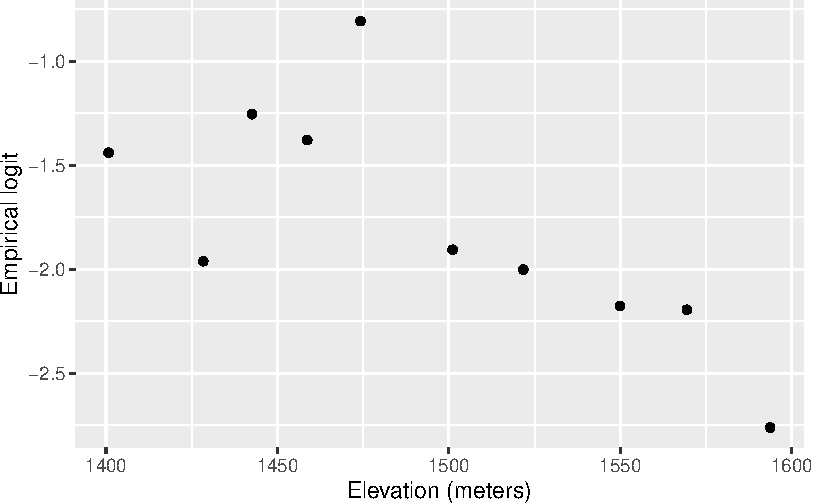
\includegraphics{03_model-fitting_files/figure-pdf/fig-elogit-elev-malkenya-1.pdf}

}

\caption{\label{fig-elogit-elev-malkenya}Plot of the empirical logit
against elevation measured in meters.}

\end{figure}

The resulting plot in Figure~\ref{fig-elogit-elev-malkenya} shows an
approximately linear relationship with decreasing values of the
empirical logit for increasing elevation. This is expected because the
cooler environment at higher altitudes is less favourable to the
development of the overall mosquito life cycle.

An alternative approach to generate a scatter plot for assessing the
association between elevation and the empirical logit would be to
aggregate the data at household level, rather than using classes of
elevation. However, this approach does not work as the one illustrated
above when only one individual is sampled for each location. In the case
of the \texttt{malkenya} data, the great majority of the locations only
include one individual making this second approach less useful than the
one illustrated.

Other more sophisticated approaches for the exploration of the
associations between covariates and binary outcomes are available. For
example, the use of the empirical logit could be avoided by using
non-parametric regression methods for Binomial outcomes (Bowman 1997),
also implemented in \texttt{sm} package in R. Our view is that a careful
exploratory analysis based on simpler methods, as those illustrated
above, can be equally effective to inform the module formulation.

\hypertarget{sec-overdispersion}{%
\subsection{Exploring overdispersion in count
data}\label{sec-overdispersion}}

One of the main advantages in the use of covariates is the ability to
attribute part of the variation of the outcome to a set of measured
variables and, hence, reduce the uncertainty of our inferences. However,
it almost always the case that the finite number of covariates at our
disposal is not enough to fully explain the variation in the outcome. In
other words, the existence of unmeasured covariates that are related to
the modelled outcome give rise to the so called residual variation. In a
standard linear regression model the extent to which we are able to
account for important covariates is directly linked to the size of the
variance of the residuals. In the case of count data, instead, this link
is less well defined and one of the main consequences of the omission of
covariates, which we address in this chapter, is \emph{overdispersion}.

Overdispersion occurs when the variability of the data is larger than
that implied by the generalized linear model (GLM) fitted to them. For
example, if we consider the Binomial distribution, the presence of
overdispersion implies that \(V(Y_i) > n_i \mu_{i}(1-\mu_i)\), where we
recall that \(n_i\) is the Binomial denominator and \(mu_i\) is the
probability of ``success'' for each of the \(n_i\) Bernoulli trials; for
a Poisson distribution with \(E(Y_i) = \mu_i\), instead, overdispersion
implies that \(V(Y_i) > \mu_{i}\).

Assessment of the overdispersion for count data can be carried out in
different ways depending on the goal of the statistical analysis. Since
the focus of this book is to illustrate how to formulate and apply
geostatistical models, the most natural approach to assess
overdispersion is through the use of generalized linear mixed models
(GLMMs). The class of GLMMs that we consider in this and the next
section are obtained by replacing the spatial Gaussian process
\(S(x_i)\) in introduced in Equation~\ref{eq-linear-predictor-ch1} with
a set of mutually independent random effects, which we denote as
\(Z_i\), and thus write
\begin{equation}\protect\hypertarget{eq-linear-predictor-glmms-ch2}{}{
g(\mu_i) = d(x_i)^\top \beta + Z_i.
}\label{eq-linear-predictor-glmms-ch2}\end{equation} The model above
accounts for the overdispersion in the data through \(Z_i\) whose
variance can be interpreted as an indicator of the amount of
overdispersion. To show this, we carry out a small simulation as
follows. For simplicity, we consider the Binomial mixed model with an
intercept only, hence
\begin{equation}\protect\hypertarget{eq-bin-glmm-example}{}{
\log\left\{\frac{\mu_i}{1-\mu_i}\right\} = \beta_0 + Z_i
}\label{eq-bin-glmm-example}\end{equation} and assume that the \(Z_i\)
follow a set of mutually independent Gaussian variables with mean 0 and
variance \(\tau^2\). In our simulation we vary \(\beta_0\) over the set
\(\{-3, -2, -1, 0, 1, 2, 3\}\) and set \(\tau^2=0.1\) and the binomial
denominators to \(n_i = 100\). For a given value of \(\beta_0\), we then
proceed through the following iterative steps.

\begin{itemize}
\item
  Simulate 10,000 values for \(Z_i\) from a Gaussian distribution with
  mean 0 and variance \(\tau^2\).
\item
  Compute the probabilities \(\mu_i\) based on
  Equation~\ref{eq-bin-glmm-example}.
\item
  Simulate 10,000 values from a Binomial model with probability of
  success \(\mu_i\) and denominator \(n_i\).
\item
  Compute the empirical variance of the counts \(y_i\) simulated in the
  previous step.
\item
  Change the value of \(\beta_0\) and repeat the previous steps, for all
  the values of \(\beta_0\).
\end{itemize}

The code below shows the implementation of the above steps in R.

\begin{Shaded}
\begin{Highlighting}[]
\CommentTok{\# Number of simulations}
\NormalTok{n\_sim }\OtherTok{\textless{}{-}} \DecValTok{10000}

\CommentTok{\# Variance of the Z\_i}
\NormalTok{tau2 }\OtherTok{\textless{}{-}} \FloatTok{0.1}

\CommentTok{\# Binomial denominator }
\NormalTok{bin\_denom }\OtherTok{\textless{}{-}} \DecValTok{100}

\CommentTok{\# Intercept values}
\NormalTok{beta0 }\OtherTok{\textless{}{-}} \FunctionTok{c}\NormalTok{(}\SpecialCharTok{{-}}\DecValTok{3}\NormalTok{, }\SpecialCharTok{{-}}\DecValTok{2}\NormalTok{, }\SpecialCharTok{{-}}\DecValTok{1}\NormalTok{, }\DecValTok{0}\NormalTok{, }\DecValTok{1}\NormalTok{, }\DecValTok{2}\NormalTok{, }\DecValTok{3}\NormalTok{)}

\CommentTok{\# Vector where we store the computed variance from}
\CommentTok{\# the simulated counts from the Binomial mixed model}
\NormalTok{var\_data }\OtherTok{\textless{}{-}} \FunctionTok{rep}\NormalTok{(}\ConstantTok{NA}\NormalTok{, }\FunctionTok{length}\NormalTok{(beta0))}


\ControlFlowTok{for}\NormalTok{(j }\ControlFlowTok{in} \DecValTok{1}\SpecialCharTok{:}\FunctionTok{length}\NormalTok{(beta0)) \{}
  \CommentTok{\# Simulation of the random effects Z\_i}
\NormalTok{  Z\_i\_sim }\OtherTok{\textless{}{-}} \FunctionTok{rnorm}\NormalTok{(n\_sim, }\AttributeTok{sd =} \FunctionTok{sqrt}\NormalTok{(tau2))}

  \CommentTok{\# Linear predictor of the Binomial mixed model}
\NormalTok{  lp }\OtherTok{\textless{}{-}}\NormalTok{ beta0[j]  }\SpecialCharTok{+}\NormalTok{ Z\_i\_sim}
  
  \CommentTok{\# Probabilities of the Binomial distribution conditional on Z\_i}
\NormalTok{  prob\_sim }\OtherTok{\textless{}{-}} \FunctionTok{exp}\NormalTok{(lp)}\SpecialCharTok{/}\NormalTok{(}\DecValTok{1}\SpecialCharTok{+}\FunctionTok{exp}\NormalTok{(lp))}
  
  \CommentTok{\# Simulation of the counts from the Binomial mixed model}
\NormalTok{  y\_i\_sim }\OtherTok{\textless{}{-}} \FunctionTok{rbinom}\NormalTok{(n\_sim, }\AttributeTok{size =}\NormalTok{ bin\_denom, }\AttributeTok{prob =}\NormalTok{ prob\_sim)}
  
  \CommentTok{\# Empirical variance from the simulated counts}
\NormalTok{  var\_data[j] }\OtherTok{\textless{}{-}} \FunctionTok{var}\NormalTok{(y\_i\_sim)}
\NormalTok{\}}

\CommentTok{\# Probabilities from the standard Binomial model (Z\_i = 0)}
\NormalTok{probs\_binomial }\OtherTok{\textless{}{-}} \FunctionTok{exp}\NormalTok{(beta0)}\SpecialCharTok{/}\NormalTok{(}\DecValTok{1}\SpecialCharTok{+}\FunctionTok{exp}\NormalTok{(beta0))}

\CommentTok{\# Variance from the standard Binomial model}
\NormalTok{var\_bimomial }\OtherTok{\textless{}{-}}\NormalTok{ bin\_denom}\SpecialCharTok{*}\NormalTok{probs\_binomial}\SpecialCharTok{*}\NormalTok{(}\DecValTok{1}\SpecialCharTok{{-}}\NormalTok{probs\_binomial)}
\end{Highlighting}
\end{Shaded}

\begin{Shaded}
\begin{Highlighting}[]
\FunctionTok{matplot}\NormalTok{(beta0, }\FunctionTok{cbind}\NormalTok{(var\_data, var\_bimomial), }\AttributeTok{type =} \StringTok{"b"}\NormalTok{, }\AttributeTok{pch =} \DecValTok{20}\NormalTok{,}
        \AttributeTok{lty =} \StringTok{"solid"}\NormalTok{, }\AttributeTok{ylab =} \StringTok{"Variance"}\NormalTok{, }\AttributeTok{xlab =} \FunctionTok{expression}\NormalTok{(beta[}\DecValTok{0}\NormalTok{]))}
\FunctionTok{legend}\NormalTok{(}\SpecialCharTok{{-}}\DecValTok{3}\NormalTok{, }\DecValTok{80}\NormalTok{, }\FunctionTok{c}\NormalTok{(}\StringTok{"Binomial mixed model"}\NormalTok{, }\StringTok{"Standard Binomial model"}\NormalTok{),}
       \AttributeTok{col=}\DecValTok{1}\SpecialCharTok{:}\DecValTok{2}\NormalTok{, }\AttributeTok{lty =} \StringTok{"solid"}\NormalTok{, }\AttributeTok{cex =} \FloatTok{0.75}\NormalTok{)}
\end{Highlighting}
\end{Shaded}

\begin{figure}[H]

{\centering 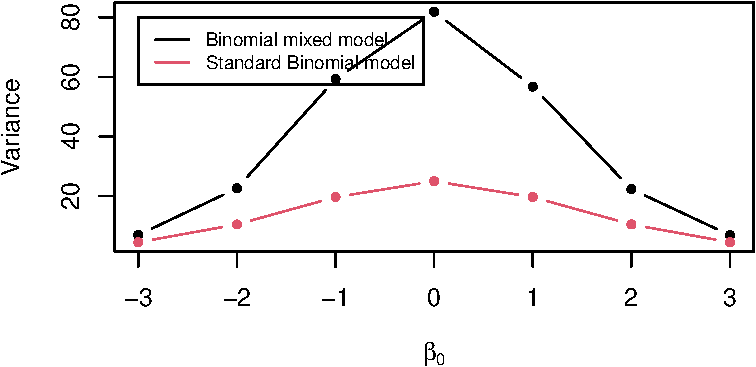
\includegraphics{03_model-fitting_files/figure-pdf/fig-var-bin-glmm-1.pdf}

}

\caption{\label{fig-var-bin-glmm}Plot of the variances of the standard
Binomial model and the Binomial mixed model (see
Equation~\ref{eq-bin-glmm-example}) against \(\beta_0\)}

\end{figure}

Figure~\ref{fig-var-bin-glmm} shows the results of the simulation. In
this figure, the red line corresponds to the variance of a standard
Binomial model, obtained by setting \(Z_i=0\) and computed as
\(n_i \mu_i (1-\mu_i)\) with
\(\mu_i = \exp\{\beta_0\}/(1+\exp\{\beta_0\})\). As expected, this plot
shows that the variance of the simulated counts from the mixed model in
Equation~\ref{eq-bin-glmm-example} exhibit a larger variance than would
be expected under the standard Binomial model. It also indicates that
the chosen value for the variance of \(Z_i\) of \(\tau^2 = 0.1\)
corresponds to a significant amount of dispersion. One way to relate
\(\tau^2\) to the amount of overdispersion is by considering that,
following from the properties of a univariate Gaussian distribution,
\emph{a priori} the \(Z_i\) will take values between
\(-1.96 \sqrt{\tau^2}\) and \(+1.96 \sqrt{\tau^2}\) with approximately
95\(\%\) probability. That implies that \(\exp\{Z_i\}\), which expresses
the effect of the random effects on the odds ratios, will be with
95\(\%\) probability between \(\exp\{-1.96 \sqrt{\tau^2}\}\) and
\(\exp\{+1.96 \sqrt{\tau^2}\}\). By replacing \(\tau^2\) with the chosen
values for the simulation, those two becomes about 0.54 and 1.86,
meaning that with the \(Z_i\) with \(95\%\) probability will have a
multiplicative effect on the odds ratios between \(0.54\) and \(1.86\).

We encourage you to do Exercise 1 and Exercise 2 at the end of this
chapter, to further explore how generalized linear mixed models can be
used as a tool to account for overdispersion.

\hypertarget{maximum-likelihood-estimation-of-generalized-linear-mixed-models-for-count-data}{%
\subsubsection{Maximum likelihood estimation of generalized linear mixed
models for count
data}\label{maximum-likelihood-estimation-of-generalized-linear-mixed-models-for-count-data}}

We now illustrate how to fit a generalize linear mixed, using the
\texttt{anopheles} data-set as an example. We consider two models: an
intercept-only model and one that uses elevation as a covariate. Let
\(\mu(x_i)\) be the number of mosquitoes captured at a location \(x_i\);
then the linear predictor with elevation as a covariate takes the form
\begin{equation}\protect\hypertarget{eq-anopheles-glmm}{}{
\log\{\mu_i\} = \beta_{0} + \beta_{1} d(x_i) + Z_i
}\label{eq-anopheles-glmm}\end{equation} where \(d(x_i)\) indicates the
elevation in meters at location \(x_i\) and the \(Z_i\) are independent
and identically distributed Gaussian variables with mean 0 and variance
\(\tau^2\). The model with an intercept only is simply obtained by
setting \(\beta_1 = 0\).

We carry out the estimation in R using the \texttt{glmer} function from
the \texttt{lme4} package (see Bates et al. (2015) for a detailed
tutorial). The \texttt{glmer} function implements the maximum likelihood
estimation for generalized linear mixed models. The code below shows how
the \texttt{glmer} is used to carry out this step for the model in
Equation~\ref{eq-anopheles-glmm} and the one withuot covariates.

\begin{Shaded}
\begin{Highlighting}[]
\CommentTok{\# Create the ID of the location}
\NormalTok{anopheles}\SpecialCharTok{$}\NormalTok{ID\_loc }\OtherTok{\textless{}{-}} \DecValTok{1}\SpecialCharTok{:}\FunctionTok{nrow}\NormalTok{(anopheles)}

\CommentTok{\# Poisson mixed model with elevation}
\NormalTok{fit\_glmer\_elev }\OtherTok{\textless{}{-}} \FunctionTok{glmer}\NormalTok{(An.gambiae }\SpecialCharTok{\textasciitilde{}} \FunctionTok{scale}\NormalTok{(elevation) }\SpecialCharTok{+}\NormalTok{ (}\DecValTok{1}\SpecialCharTok{|}\NormalTok{ID\_loc), }\AttributeTok{family =}\NormalTok{ poisson, }
                        \AttributeTok{data =}\NormalTok{ anopheles, }\AttributeTok{nAGQ =} \DecValTok{25}\NormalTok{)}

\CommentTok{\# Poisson mixed model with intercept only}
\NormalTok{fit\_glmer\_int }\OtherTok{\textless{}{-}} \FunctionTok{glmer}\NormalTok{(An.gambiae }\SpecialCharTok{\textasciitilde{}}\NormalTok{ (}\DecValTok{1}\SpecialCharTok{|}\NormalTok{ID\_loc), }\AttributeTok{family =}\NormalTok{ poisson, }
                        \AttributeTok{data =}\NormalTok{ anopheles, }\AttributeTok{nAGQ =} \DecValTok{25}\NormalTok{)}
\end{Highlighting}
\end{Shaded}

To fit the model with \texttt{glmer}, we first must create a variable in
our data-set that allows us to identify the location associated with
each count. In this case, since every row corresponds to a different
location, we simply use the row number to identify the locations and
save this in the \texttt{ID\_loc} variable. The random effects \(Z_i\)
are then included in the model by adding
\texttt{(1\ \textbar{}\ ID\_loc)} in the formula of the \texttt{glmer}
function.

When introducing the variable elevation, we standardize the variable so
that its mean is 0 and its variance is 1. This is done to aid the
convergence of the algorithm used to fit the model and it is generally
considered good practice, especially when many variables with different
scales are used as covariates. However, we emphasize that standardizing
a variable does not affect the fit of the model to the data. This is
because the model with the standardized variable is a reparametrization
of the model with the unstandardized variable. In other words, a model
that uses standardized covariates only attaches a different
interpretation to its regression coefficients while maintaining the same
goodness of fit of the model with that uses the covariates on their
original scale.

The argument \texttt{nAGQ} is used to define the precision of the
approximation of the maximum likelihood estimation algorithm. By default
\texttt{nAGQ\ =\ 1}, which corresponds to the Laplace approximation.
Values for \texttt{nAGQ} larger than 1 are used to define the number of
points of the adaptive Gaussian-Hermite quadrature. The general
principle is that the larger \texttt{nAGQ} the better, but at the
expense of an increased computing time. Based on the guidelines and help
pages of the \texttt{lme4} package, it is stated that a reasonable value
for \texttt{nAGQ} is 25. For more technical details on this aspect, we
refer the reader to Bates et al. (2015).

We can now look at the summary of the fitted models to the mosquitoes
data-set.

\begin{Shaded}
\begin{Highlighting}[]
\DocumentationTok{\#\#\# Summary of the model with elevation}
\FunctionTok{summary}\NormalTok{(fit\_glmer\_elev)}
\DocumentationTok{\#\# Generalized linear mixed model fit by maximum likelihood (Adaptive}
\DocumentationTok{\#\#   Gauss{-}Hermite Quadrature, nAGQ = 25) [glmerMod]}
\DocumentationTok{\#\#  Family: poisson  ( log )}
\DocumentationTok{\#\# Formula: An.gambiae \textasciitilde{} scale(elevation) + (1 | ID\_loc)}
\DocumentationTok{\#\#    Data: anopheles}
\DocumentationTok{\#\# }
\DocumentationTok{\#\#      AIC      BIC   logLik deviance df.resid }
\DocumentationTok{\#\#    291.8    300.1   {-}142.9    285.8      113 }
\DocumentationTok{\#\# }
\DocumentationTok{\#\# Scaled residuals: }
\DocumentationTok{\#\#      Min       1Q   Median       3Q      Max }
\DocumentationTok{\#\# {-}0.89574 {-}0.42469 {-}0.09483  0.29445  0.53352 }
\DocumentationTok{\#\# }
\DocumentationTok{\#\# Random effects:}
\DocumentationTok{\#\#  Groups Name        Variance Std.Dev.}
\DocumentationTok{\#\#  ID\_loc (Intercept) 0.7146   0.8453  }
\DocumentationTok{\#\# Number of obs: 116, groups:  ID\_loc, 116}
\DocumentationTok{\#\# }
\DocumentationTok{\#\# Fixed effects:}
\DocumentationTok{\#\#                  Estimate Std. Error z value Pr(\textgreater{}|z|)    }
\DocumentationTok{\#\# (Intercept)       1.53042    0.09365  16.342   \textless{}2e{-}16 ***}
\DocumentationTok{\#\# scale(elevation) {-}0.19794    0.08950  {-}2.212    0.027 *  }
\DocumentationTok{\#\# {-}{-}{-}}
\DocumentationTok{\#\# Signif. codes:  0 \textquotesingle{}***\textquotesingle{} 0.001 \textquotesingle{}**\textquotesingle{} 0.01 \textquotesingle{}*\textquotesingle{} 0.05 \textquotesingle{}.\textquotesingle{} 0.1 \textquotesingle{} \textquotesingle{} 1}
\DocumentationTok{\#\# }
\DocumentationTok{\#\# Correlation of Fixed Effects:}
\DocumentationTok{\#\#             (Intr)}
\DocumentationTok{\#\# scale(lvtn) 0.036}

\DocumentationTok{\#\#\# Summary of the model with the intercept only}
\FunctionTok{summary}\NormalTok{(fit\_glmer\_int)}
\DocumentationTok{\#\# Generalized linear mixed model fit by maximum likelihood (Adaptive}
\DocumentationTok{\#\#   Gauss{-}Hermite Quadrature, nAGQ = 25) [glmerMod]}
\DocumentationTok{\#\#  Family: poisson  ( log )}
\DocumentationTok{\#\# Formula: An.gambiae \textasciitilde{} (1 | ID\_loc)}
\DocumentationTok{\#\#    Data: anopheles}
\DocumentationTok{\#\# }
\DocumentationTok{\#\#      AIC      BIC   logLik deviance df.resid }
\DocumentationTok{\#\#    294.6    300.1   {-}145.3    290.6      114 }
\DocumentationTok{\#\# }
\DocumentationTok{\#\# Scaled residuals: }
\DocumentationTok{\#\#      Min       1Q   Median       3Q      Max }
\DocumentationTok{\#\# {-}0.73816 {-}0.42718 {-}0.06941  0.26564  0.45022 }
\DocumentationTok{\#\# }
\DocumentationTok{\#\# Random effects:}
\DocumentationTok{\#\#  Groups Name        Variance Std.Dev.}
\DocumentationTok{\#\#  ID\_loc (Intercept) 0.761    0.8724  }
\DocumentationTok{\#\# Number of obs: 116, groups:  ID\_loc, 116}
\DocumentationTok{\#\# }
\DocumentationTok{\#\# Fixed effects:}
\DocumentationTok{\#\#             Estimate Std. Error z value Pr(\textgreater{}|z|)    }
\DocumentationTok{\#\# (Intercept)  1.52849    0.09584   15.95   \textless{}2e{-}16 ***}
\DocumentationTok{\#\# {-}{-}{-}}
\DocumentationTok{\#\# Signif. codes:  0 \textquotesingle{}***\textquotesingle{} 0.001 \textquotesingle{}**\textquotesingle{} 0.01 \textquotesingle{}*\textquotesingle{} 0.05 \textquotesingle{}.\textquotesingle{} 0.1 \textquotesingle{} \textquotesingle{} 1}
\end{Highlighting}
\end{Shaded}

From the summary of the model that uses elevation, we observe the that
the estimated regression coefficient \(\beta_{1}\) is statistically
significant different from 0. The interpretation of the estimated
regression coefficient is the following: for an increase of about 100
meters in elevation, all other things being equal, the average number of
mosquitoes decreases by about
\(100\% \times [1-\exp\{-0.19794\}] \approx 18\%\). Note that when using
a standardized variable, a unit increase for this corresponds to an
increase in the original unstandardized variable equal to its standard
deviation, which for the \texttt{elevation} variable is about 100
meters.

From the summaries of the two models, under \texttt{Random\ effects:},
we obtain the estimates associates with the random effects introduced in
the model. In this case, since we only have introduced \(Z_i\), this
part of summary provides the maximum likelihood estimate for \(\tau^2\),
the variance of \(Z_i\), which found on the line where \texttt{ID\_loc}
is printed. We then observe that the estimates for \(\tau^2\) for the
intercept-only model is \texttt{0.761}, whilst for the model with
elevation this is \texttt{0.7146}. Note that the figures reported under
\texttt{Std.Dev.} are simply the square root of the value reported under
\texttt{Variance}. As expected, the introduction of elevation
contributes to the explanation of the residual variation captured by
\(Z_i\), though by a very small amount. The estimated values of
\(\tau^2\) thus suggest that there is extra-Binomial variation in the
data that is not account for by elevation.

In the next section, we will illustrate how to assess the presence of
residual correlation for continuous measurements and overdispersed count
data.

\hypertarget{sec-expl-spatial}{%
\subsection{Exploring residual spatial
correlation}\label{sec-expl-spatial}}

In its most basic form, the concept of spatial correlation can be
succinctly encapsulated by Tobler (1970) first law of geography, which
posits that ``everything is interconnected, but objects in close
proximity exhibit stronger relationships than those situated farther
apart.'' After we have identified the key variables to introduce as
covariates in the model (Section~\ref{sec-expl-assoc}) and, in the case
of count data, assessed the presence of overdispersion
(Section~\ref{sec-overdispersion}), our final exploratory step consists
of assessing whether the residuals of the non spatial model show
evidence of spatial correlation. Hence, in geostatistical modelling, the
interest is not in the spatial correlation of the data, but rather on
understanding whether the variation in the outcome unexplained by the
covariates exhibits spatial correlation. We call this \emph{residual
spatial correlation}, to emphasize that spatial correlation is a concept
relative to the covariates that we have introduced in the model.

In the context of geostatistical analysis, the tool that is generally
used to assess the residual spatial correlation is the the so called
\emph{empirical variogram}. Before looking at the mathematical
definition of the empirical variogram, let us consider a generalized
linear mixed model as expressed in
Equation~\ref{eq-linear-predictor-glmms-ch2}. Our goal is then to
question the assumption of independently distributed random effects
\(Z_i\) by asking whether the \(Z_i\) show evidence of spatial
correlation. Let \(Z_i\) and \(Z_j\) be two random effects that are
associate with two different locations \(x_i\) and \(x_j\),
respectively, and let us take the squared difference between the two
\begin{equation}\protect\hypertarget{eq-squared-diff}{}{
V_{ij} = (Z_i - Z_j)^2.
}\label{eq-squared-diff}\end{equation} How does the spatial correlation
affect the value of \(V_{ij}\)? To answer this question, we can refer to
the aforementioned Tobler's law of geography. When \(x_i\) and \(x_j\)
will be closer to each other, then \(Z_i\) and \(Z_j\) will also tend to
be more similar to each other, thus making \(V_{ij}\) smaller, on
average. On the contrary, when \(x_i\) and \(x_j\) will be further
apart, then \(V_{ij}\) will become larger, on average. We can then
construct the empirical variogram by considering all possible pairs of
locations \(x_i\) and \(x_j\), for which we then compute \(V_{ij}\) and
plot this against the distance between \(x_i\) and \(x_j\), which we
denote as \(u_{ij}\). If there is spatial correlation in the random
effects \(Z_i\), then this will manifest as an average increase in the
\(V_{ij}\) as \(u_{ij}\) increases. However, there are still two issues
that we have to address before we can generate and plot the empirical
variogram.

The first issue is that we do not observe \(Z_i\) as, by definition,
this is a latent variable. Hence, we require an estimate for \(Z_i\)
which we can then feed into \(V_{ij}\). To emphasize this point, from
now on, we shall replace Equation~\ref{eq-squared-diff} with
\begin{equation}\protect\hypertarget{eq-hat-squared-diff}{}{
\hat{V}_{ij} = (\hat{Z}_{i} - \hat{Z}_j)^2.
}\label{eq-hat-squared-diff}\end{equation} Several options are available
for estimating \(Z_{i}\). Our choice is to use the model of the
predictive distribution of \(Z_i\), that is the distribution of
\(Z_{i}\) conditioned to the data \(y_i\). This estimator for \(Z_i\) is
also readily available from the output of the \texttt{lmer} and
\texttt{glmer} functions of the \texttt{lme4} package, as we will
illustrate later in our example in this section.

The second issue is that if simply plot \(\hat{V}_{ij}\) against the
distances \(u_{ij}\) (also knwon as \emph{cloud variogram}), due to the
high noiseness in the \(\hat{V}_{ij}\), it may be quite difficult to
assess the presence of an increasing trend in the \(\hat{V}_{ij}\) and
thus detect spatial correlation. Hence, it is general practice to group
the distances \(u_{ij}\) into classes, say \(\mathcal{U}\), and then
take average of all the \(\hat{V}_{ij}\) that fall within
\(\mathcal{U}\).

We can now write the formal definition of the empirical variogram as
\begin{equation}\protect\hypertarget{eq-empirical-variogram}{}{
\hat{V}(\mathcal{U}) = \frac{1}{2 |\mathcal{U}|} \sum_{(i, j): (u_i, u_j) \in \mathcal{U}} \hat{V}_{ij}
}\label{eq-empirical-variogram}\end{equation} where \(|\mathcal{U}|\)
denotes the number of pairs of locations that fall within the distance
class \(\mathcal{U}\). The rationale behind dividing by 2 in
\(1/2 |\mathcal{U}|\) from the above equation, will be elucidated in
Section~\ref{sec-linear-model}, and there is no need for us to delve
into this matter at this juncture. When creating the empirical variogram
plot, we select the midpoint values of the distance classes
\(\mathcal{U}\) to represent the x-axis values.

Before we can evaluate residual spatial correlation, there remains one
crucial concern: relying solely on a visual inspection of the empirical
variogram is susceptible to human subjectivity. Furthermore, it is worth
noting that even a seemingly upward trend observed in the empirical
variogram might be merely a product of random fluctuations, rather than
a reliable indication of actual residual spatial correlation. To address
these concerns and enhance the objectivity of the use of the empirical
variogram, one approach would involve comparing the observed empirical
variogram pattern with those generated in the absence of spatial
correlation. Following this principle, we then use a permutation test
that allows us to generate empirical variograms under the assumption of
absence of spatial correlation through the following iterative steps.

\begin{enumerate}
\def\labelenumi{\arabic{enumi}.}
\item
  Permute the order of the locations in the data-set while keeping
  everything else fixed.
\item
  Compute the empirical variogram \(\hat{V}(\mathcal{U})\) for the
  permuted data-set.
\item
  Repeat 1 and 2 a large number of times, say 10,000.
\item
  Use the resulting 10,000 empirical varigorams to compute 95\(\%\)
  confidence intervals, by taking the 0.025 and 0.975 quantiles of these
  for each distance class \(\hat{V}(\mathcal{U})\).
\item
  If the observed empirical variogram falls fully within the envelope
  generated in the previous point, we then conclude that the data do not
  exhibit residual spatial correlation. If, instead, the observed
  empirical variogram partly falls outside the envelope we conclude that
  the data do exhibit residual spatial correlation.
\end{enumerate}

We now show an application of all the concepts introduced in this
section to the Liberia data on river-blindness.

\hypertarget{sec-empirical-variog-bin}{%
\subsubsection{Example: assessing spatial correlation for the Liberia
data}\label{sec-empirical-variog-bin}}

We consider the Binomial mixed model that uses the log-transformed
elevation as a covariate to model river blindness prevalence, hence
\begin{equation}\protect\hypertarget{eq-liberia-bin-mixed-elev}{}{
\log\left\{\frac{p(x_i)}{1-p(x_i)}\right\} = \beta_{0} + \beta_{1}\log\{e(x_i)\} + Z_i
}\label{eq-liberia-bin-mixed-elev}\end{equation} where \(e(x_i)\) is the
elevation in meters at location \(x_i\) and the \(Z_i\) are i.i.d.
Gaussian variables with mean 0 and variance \(\tau^2\). We first fit the
model above using the \texttt{glmer} function.

\begin{Shaded}
\begin{Highlighting}[]
\CommentTok{\# Convert the data{-}set into an sf object}
\NormalTok{liberia }\OtherTok{\textless{}{-}} \FunctionTok{st\_as\_sf}\NormalTok{(liberia, }\AttributeTok{coords =} \FunctionTok{c}\NormalTok{(}\StringTok{"lat"}\NormalTok{, }\StringTok{"long"}\NormalTok{), }\AttributeTok{crs =} \DecValTok{4326}\NormalTok{)}


\CommentTok{\# Create the ID of the location}
\NormalTok{liberia}\SpecialCharTok{$}\NormalTok{ID\_loc }\OtherTok{\textless{}{-}} \DecValTok{1}\SpecialCharTok{:}\FunctionTok{nrow}\NormalTok{(liberia)}

\CommentTok{\# Binomial mixed model with log{-}elevation}
\NormalTok{fit\_glmer\_lib }\OtherTok{\textless{}{-}} \FunctionTok{glmer}\NormalTok{(}\FunctionTok{cbind}\NormalTok{(npos, ntest) }\SpecialCharTok{\textasciitilde{}} \FunctionTok{log}\NormalTok{(elevation) }\SpecialCharTok{+}\NormalTok{ (}\DecValTok{1}\SpecialCharTok{|}\NormalTok{ID\_loc), }\AttributeTok{family =}\NormalTok{ binomial,}
                        \AttributeTok{data =}\NormalTok{ liberia, }\AttributeTok{nAGQ =} \DecValTok{25}\NormalTok{)}

\FunctionTok{summary}\NormalTok{(fit\_glmer\_lib)}
\end{Highlighting}
\end{Shaded}

\begin{verbatim}
Generalized linear mixed model fit by maximum likelihood (Adaptive
  Gauss-Hermite Quadrature, nAGQ = 25) [glmerMod]
 Family: binomial  ( logit )
Formula: cbind(npos, ntest) ~ log(elevation) + (1 | ID_loc)
   Data: liberia

     AIC      BIC   logLik deviance df.resid 
   127.9    135.4    -61.0    121.9       87 

Scaled residuals: 
     Min       1Q   Median       3Q      Max 
-2.46033 -0.63341 -0.07633  0.61995  3.12732 

Random effects:
 Groups Name        Variance Std.Dev.
 ID_loc (Intercept) 0.003097 0.05565 
Number of obs: 90, groups:  ID_loc, 90

Fixed effects:
               Estimate Std. Error z value Pr(>|z|)    
(Intercept)    -2.96292    0.21184 -13.987  < 2e-16 ***
log(elevation)  0.26143    0.04071   6.422 1.35e-10 ***
---
Signif. codes:  0 '***' 0.001 '**' 0.01 '*' 0.05 '.' 0.1 ' ' 1

Correlation of Fixed Effects:
            (Intr)
log(elevtn) -0.981
\end{verbatim}

From the output, we observe that the estimate for \(\tau^2\) is about
0.003, indicating a moderate level of overdispersion in the data.

\begin{Shaded}
\begin{Highlighting}[]
\NormalTok{liberia}\SpecialCharTok{$}\NormalTok{Z\_hat }\OtherTok{\textless{}{-}} \FunctionTok{ranef}\NormalTok{(fit\_glmer\_lib)}\SpecialCharTok{$}\NormalTok{ID\_loc[,}\DecValTok{1}\NormalTok{]}
\end{Highlighting}
\end{Shaded}

Throuhg the function \texttt{ranef} when extract the estimates of the
random effects \(Z_i\) and save these in the data set. We then use the
function \texttt{s\_variogram} from the \texttt{RiskMap} package to
compute the empirical varigoram for the estimated \(\hat{Z}_i\).

\begin{Shaded}
\begin{Highlighting}[]
\NormalTok{liberia\_variog }\OtherTok{\textless{}{-}} \FunctionTok{s\_variogram}\NormalTok{(}\AttributeTok{data =}\NormalTok{ liberia,}
                              \AttributeTok{variable =} \StringTok{"Z\_hat"}\NormalTok{,}
                              \AttributeTok{bins =} \FunctionTok{c}\NormalTok{(}\DecValTok{15}\NormalTok{, }\DecValTok{30}\NormalTok{, }\DecValTok{40}\NormalTok{, }\DecValTok{80}\NormalTok{, }\DecValTok{120}\NormalTok{,}
                                       \DecValTok{160}\NormalTok{, }\DecValTok{200}\NormalTok{, }\DecValTok{250}\NormalTok{, }\DecValTok{300}\NormalTok{, }\DecValTok{350}\NormalTok{),}
                              \AttributeTok{scale\_to\_km =} \ConstantTok{TRUE}\NormalTok{,}
                              \AttributeTok{n\_permutation =} \DecValTok{10000}\NormalTok{)}
\end{Highlighting}
\end{Shaded}

Through the argument \texttt{bins} we can specify the the classes of
distance, previously denoted by \(\mathcal{U}\); check the help page of
\texttt{s\_variogram} to see how this is defined by default. The value
passed to \texttt{bins} in the code above correspond to define the
following classes of distance \(\mathcal{U}\): \([15, 30]\),
\((30, 40]\) and so forth, with the last class being \([350, +\infty)\),
i.e.~all pairs of locations whose distances are above 350km. The
argument \texttt{n\_permutation} allows the user to specify the number
of permutations that are performed the generate the envelope for absence
of spatial correlation previously described.

\begin{Shaded}
\begin{Highlighting}[]
\FunctionTok{dist\_summaries}\NormalTok{(}\AttributeTok{data =}\NormalTok{ liberia,}
               \AttributeTok{scale\_to\_km =} \ConstantTok{TRUE}\NormalTok{)}
\DocumentationTok{\#\# $min}
\DocumentationTok{\#\# [1] 3.34536}
\DocumentationTok{\#\# }
\DocumentationTok{\#\# $max}
\DocumentationTok{\#\# [1] 533.0733}
\DocumentationTok{\#\# }
\DocumentationTok{\#\# $mean}
\DocumentationTok{\#\# [1] 206.7424}
\DocumentationTok{\#\# }
\DocumentationTok{\#\# $median}
\DocumentationTok{\#\# [1] 192.6496}
\end{Highlighting}
\end{Shaded}

The \texttt{dist\_summaries} function within the \texttt{RiskMap}
package can be used for gauging the extent of the area covered by your
dataset, aiding in the selection of appropriate values to be passed to
the \texttt{bins} argument. In the provided output above, we can observe
that for the Liberia dataset, the minimum and maximum distances span
approximately 3km and 533km, respectively. While there is not a
one-size-fits-all recommendation for setting \texttt{bins}, two
fundamental principles should inform your decision-making. Firstly, it
is advisable to avoid choosing overly large distance intervals, as the
uncertainty associated with the empirical variogram tends to increase
with distance due to fewer available pairs of observations for
estimation. Secondly, especially when spatial correlation is not strong,
it is crucial to carefully explore the behavior of the variogram at
smaller distances. Consequently, it is generally advisable to experiment
with different \texttt{bins} configurations and observe how they impact
the pattern of the empirical variogram.

\begin{Shaded}
\begin{Highlighting}[]
\FunctionTok{plot\_s\_variogram}\NormalTok{(liberia\_variog,}
                 \AttributeTok{plot\_envelope =} \ConstantTok{TRUE}\NormalTok{)}
\end{Highlighting}
\end{Shaded}

\begin{figure}[H]

{\centering 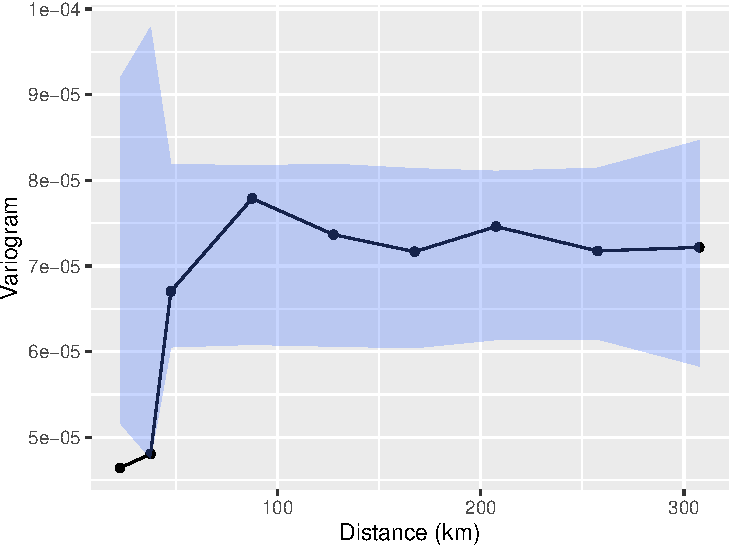
\includegraphics{03_model-fitting_files/figure-pdf/fig-liberia-variog-1.pdf}

}

\caption{\label{fig-liberia-variog}Plot of the empirical variogram
(solid line) computed using the estimated random effects from the model
in Equation~\ref{eq-liberia-bin-mixed-elev}. The blue shaded area is the
95\% confidence level envelope generated using the permutation procedure
described in Section~\ref{sec-expl-spatial}.}

\end{figure}

Finally, the \texttt{plot\_s\_variogram} function enables us to
visualize the empirical variogram and, through the
\texttt{plot\_envelope} argument, include the envelope generated by the
permutation procedure. As illustrated in
Figure~\ref{fig-liberia-variog}, we observe that the empirical variogram
falls outside the envelope at relatively short distances, typically
below 30km. However, for distances exceeding 30km, the behavior of the
empirical variogram does not significantly differ from variograms
generated under the assumption of spatial independence. In summary, we
interpret the evidence presented in Figure~\ref{fig-liberia-variog} as
indicative of residual spatial correlation within the data.
Nevertheless, it is essential to exercise caution when attempting to
ascertain the scale of the spatial correlation using the empirical
variogram. As we will emphasize throughout this book, the empirical
variogram's sensitivity to the choice of bins values renders it an
unreliable tool for drawing statistical inferences. In other words, we
advocate employing the empirical variogram primarily to assess the
presence of residual correlation.

\hypertarget{sec-empirical-variog-lm}{%
\subsubsection{Exploring residual spatial correlation with linear
Guassian models}\label{sec-empirical-variog-lm}}

When using a linear model to assess spatial correlation, it is important
to distinguish two cases: 1) when the data contain only one location per
location; 2) when more than one observation per location is available.
We now consider each of these two scenarios separately.

\hypertarget{one-observation-per-location}{%
\paragraph{One observation per
location}\label{one-observation-per-location}}

To illustrate the use of the variogram under this scenario, we shall use
the Gailicia data on lead concentration in moss samples. The simplest
possible model for the data is a standard linear model without
covariates which assumes independence among the observations, hence
\begin{equation}\protect\hypertarget{eq-std-lm-galicia}{}{
Y_i = \beta_0 + U_i
}\label{eq-std-lm-galicia}\end{equation} where the \(U_i\) are i.i.d.
Gaussian variables with mean zero and variance \(\omega^2\). At this
stage, our goal is then to assess whether the assumption of independence
for the \(Z_i\) is supported by the data or whether there is evidence of
spatial correlation. However, the measurement error of the device may be
present as part of the natural random variation in \(Z_i\) which might
mask the detection of spatial correlation using the residuals \(Z_i\)
challenging, especially is the measurement error dominates the spatial
variation of the data. One would be tempted to introduce an additional,
location-specific random effect, say \(Z_i\) with mean zero and variance
\(\tau^2\) and fit the model
\begin{equation}\protect\hypertarget{eq-std-lm2-galicia}{}{
Y_i = \beta_0 + Z_i + U_i,
}\label{eq-std-lm2-galicia}\end{equation} where we interpret \(U_i\) as
random variation due to the measurement device and \(Z_i\) as a random
effect accounting for unmeasured covariates that contribute to the
variation between locations in lead concentration. However, the model in
Equation~\ref{eq-std-lm2-galicia} is not identifiable because we cannot
disentangle the separate contributions of \(Z_i\) and \(U_i\) from the
variation of the data, unless: a) we know the precision of the
measurement device, \(\omega\) (recall that \(\omega^2\) is the variance
of \(U_i\)); b) or, if we do not know \(\omega\), we can then separate
the two sources of variation only if we have multiple observations per
location (the scenario which we shall consider in the next section).

For the Galicia data, for we do not know the measurement device
precision and we only have one observation per location. However, this
does not prevent us from using the variogram based on the residuals from
Equation~\ref{eq-std-lm-galicia}, while keeping in mind the limitations
and uncertainty that are inherent to this exploratory tool as remarked
at the end of the last paragraph.

\begin{Shaded}
\begin{Highlighting}[]
\CommentTok{\# Fitting of the linear model and extraction of the residuals  }
\NormalTok{lm\_fit }\OtherTok{\textless{}{-}} \FunctionTok{lm}\NormalTok{(}\FunctionTok{log}\NormalTok{(lead) }\SpecialCharTok{\textasciitilde{}} \DecValTok{1}\NormalTok{, }\AttributeTok{data =}\NormalTok{ galicia)}
\NormalTok{galicia}\SpecialCharTok{$}\NormalTok{residuals }\OtherTok{\textless{}{-}}\NormalTok{ lm\_fit}\SpecialCharTok{$}\NormalTok{residuals}

\CommentTok{\# Convert the galicia data frame into an "sf" object}
\NormalTok{galicia\_sf }\OtherTok{\textless{}{-}} \FunctionTok{st\_as\_sf}\NormalTok{(galicia, }\AttributeTok{coords =} \FunctionTok{c}\NormalTok{(}\StringTok{"x"}\NormalTok{, }\StringTok{"y"}\NormalTok{), }\AttributeTok{crs =} \DecValTok{32629}\NormalTok{)}

\CommentTok{\# Compute the variogram, using the residuals from the linear model fit,}
\CommentTok{\# and the 95\% confidence level envelope for spatial independence}
\NormalTok{galicia\_variog }\OtherTok{\textless{}{-}} \FunctionTok{s\_variogram}\NormalTok{(galicia\_sf, }\AttributeTok{variable =} \StringTok{"residuals"}\NormalTok{,}
                              \AttributeTok{scale\_to\_km =} \ConstantTok{TRUE}\NormalTok{,}
                              \AttributeTok{bins =} \FunctionTok{seq}\NormalTok{(}\DecValTok{10}\NormalTok{, }\DecValTok{140}\NormalTok{, }\AttributeTok{length =} \DecValTok{15}\NormalTok{),}
                              \AttributeTok{n\_permutation =} \DecValTok{10000}\NormalTok{)}

\CommentTok{\# Plotting the results}
\FunctionTok{plot\_s\_variogram}\NormalTok{(galicia\_variog, }\AttributeTok{plot\_envelope =} \ConstantTok{TRUE}\NormalTok{)}
\end{Highlighting}
\end{Shaded}

\begin{figure}[H]

{\centering 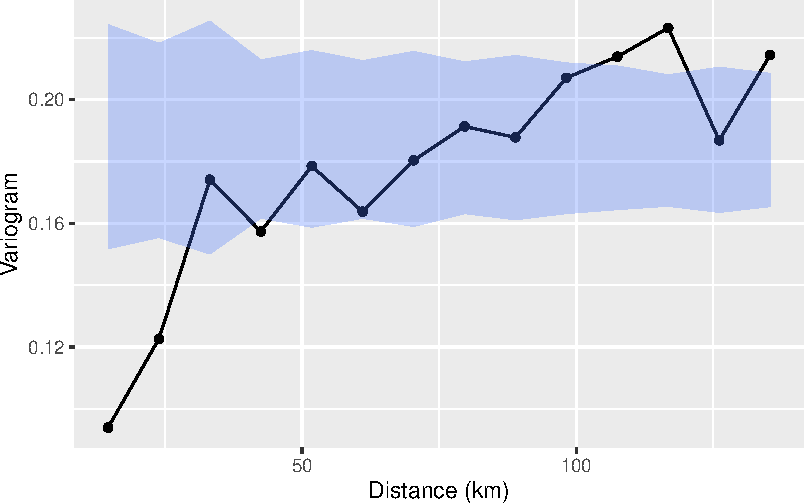
\includegraphics{03_model-fitting_files/figure-pdf/fig-galicia-variog-1.pdf}

}

\caption{\label{fig-galicia-variog}Plot of the empirical variogram
(solid line) computed using the estimated residuals from the model in
Equation~\ref{eq-std-lm-galicia}. The blue shaded area is the 95\%
confidence level envelope generated using the permutation procedure
described in Section~\ref{sec-expl-spatial}.}

\end{figure}

In the code above, we first fit the linear model in
Equation~\ref{eq-std-lm-galicia} and then extract the residuals from
this. Note that for this simple model, the residuals of the model are
obtained by simply centering the outcome to zero by subtracting its
mean. However, for more complex linear models that use covariates the
computation of the residuals is more involved and can be carried out
through a simple extension of the code above by specifying an
appropriate \texttt{formula} in the \texttt{lm} function.

Figure~\ref{fig-galicia-variog} shows the empirical variogram and the
95\% envelope for spatial independence. This clearly shows that the
measurement of lead concentration are spatially correlated.

\hypertarget{sec-explanal-lm}{%
\paragraph{More than one observation per
location}\label{sec-explanal-lm}}

For the case of more than one observation per location, we shall
consider the \texttt{italy\_sim} data-set. This data-set contains 10
observations per location, for a total of 200 locations. The variable
\texttt{ID\_loc} is a numeric indicator that can be used to identify the
location each observation belong to. For this data-set, we use the
population density, named \texttt{pop\_dens}, as a log-transformed
covariate; we leave you as an exercise to assess that is a reasonable
modelling choice.

To specify a non-spatial mixed model for the outcome, we then use two
subscripts: \(i\) to identify a given location; \(j\) to identify the
\(j\)-th observation for a given location \(i\). We denote as \(Z_i\)
the location-specific random effect ans as \(U_{ij}\) the random
variation due to the measurement error inherent to each observation.
Hence, we write
\begin{equation}\protect\hypertarget{eq-italy-sim-lmm}{}{
Y_{ij} = \beta_0 + \beta_1 \log\{d(x_i)\} + Z_i + U_{ij},
}\label{eq-italy-sim-lmm}\end{equation} where \(d(x_i)\) is the
population density at location \(x_i\); as before, we use \(\tau^2\) and
\(\omega^2\) to denote the variances of \(Z_i\) and \(U_{ij}\),
respectively. To fit this model to the data we use the \texttt{lmer}
function from the \texttt{lme4} package.

\begin{Shaded}
\begin{Highlighting}[]
\CommentTok{\# Fitting a linear mixed model to the italy\_sim data{-}set}
\CommentTok{\# See main text for model specification}
\NormalTok{lmer\_fit }\OtherTok{\textless{}{-}} \FunctionTok{lmer}\NormalTok{(y }\SpecialCharTok{\textasciitilde{}} \FunctionTok{log}\NormalTok{(pop\_dens) }\SpecialCharTok{+}\NormalTok{ (}\DecValTok{1}\SpecialCharTok{|}\NormalTok{ID\_loc), }\AttributeTok{data =}\NormalTok{ italy\_sim)}

\FunctionTok{summary}\NormalTok{(lmer\_fit)}
\DocumentationTok{\#\# Linear mixed model fit by REML [\textquotesingle{}lmerMod\textquotesingle{}]}
\DocumentationTok{\#\# Formula: y \textasciitilde{} log(pop\_dens) + (1 | ID\_loc)}
\DocumentationTok{\#\#    Data: italy\_sim}
\DocumentationTok{\#\# }
\DocumentationTok{\#\# REML criterion at convergence: 3390.9}
\DocumentationTok{\#\# }
\DocumentationTok{\#\# Scaled residuals: }
\DocumentationTok{\#\#      Min       1Q   Median       3Q      Max }
\DocumentationTok{\#\# {-}2.85209 {-}0.64198 {-}0.01832  0.66014  3.01870 }
\DocumentationTok{\#\# }
\DocumentationTok{\#\# Random effects:}
\DocumentationTok{\#\#  Groups   Name        Variance Std.Dev.}
\DocumentationTok{\#\#  ID\_loc   (Intercept) 2.5006   1.5813  }
\DocumentationTok{\#\#  Residual             0.1959   0.4426  }
\DocumentationTok{\#\# Number of obs: 2000, groups:  ID\_loc, 200}
\DocumentationTok{\#\# }
\DocumentationTok{\#\# Fixed effects:}
\DocumentationTok{\#\#               Estimate Std. Error t value}
\DocumentationTok{\#\# (Intercept)   {-}0.40448    0.57613  {-}0.702}
\DocumentationTok{\#\# log(pop\_dens)  1.33798    0.07643  17.506}
\DocumentationTok{\#\# }
\DocumentationTok{\#\# Correlation of Fixed Effects:}
\DocumentationTok{\#\#             (Intr)}
\DocumentationTok{\#\# log(pp\_dns) {-}0.981}

\CommentTok{\# Incorporating the estimated random effects into the data}
\NormalTok{italy\_sim}\SpecialCharTok{$}\NormalTok{rand\_eff }\OtherTok{\textless{}{-}}\FunctionTok{ranef}\NormalTok{(lmer\_fit)}\SpecialCharTok{$}\NormalTok{ID\_loc[italy\_sim}\SpecialCharTok{$}\NormalTok{ID\_loc,}\DecValTok{1}\NormalTok{]}

\CommentTok{\# Converting the italy\_sim data frame into an "sf" object }
\NormalTok{italy\_sim\_sf }\OtherTok{\textless{}{-}} \FunctionTok{st\_as\_sf}\NormalTok{(italy\_sim, }\AttributeTok{coords=}\FunctionTok{c}\NormalTok{(}\StringTok{"x1"}\NormalTok{, }\StringTok{"x2"}\NormalTok{), }\AttributeTok{crs =} \DecValTok{32634}\NormalTok{)}

\CommentTok{\# Compute the variogram, using the random effects from the linear mixed model fit,}
\CommentTok{\# and the 95\% confidence level envelope for spatial independence}
\NormalTok{italy\_sim\_variog }\OtherTok{\textless{}{-}} \FunctionTok{s\_variogram}\NormalTok{(italy\_sim\_sf, }\AttributeTok{variable =} \StringTok{"rand\_eff"}\NormalTok{, }
                                \AttributeTok{scale\_to\_km =} \ConstantTok{TRUE}\NormalTok{,}
                                \AttributeTok{n\_permutation =} \DecValTok{200}\NormalTok{)}

\CommentTok{\# Plotting the results}
\FunctionTok{plot\_s\_variogram}\NormalTok{(italy\_sim\_variog, }\AttributeTok{plot\_envelope =} \ConstantTok{TRUE}\NormalTok{)}
\end{Highlighting}
\end{Shaded}

\begin{figure}[H]

{\centering 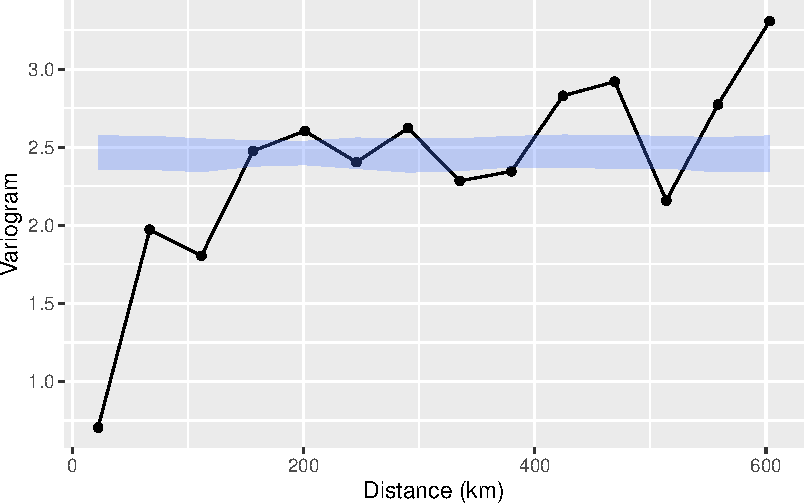
\includegraphics{03_model-fitting_files/figure-pdf/fig-italy-sim-variog-1.pdf}

}

\caption{\label{fig-italy-sim-variog}Plot of the empirical variogram
(solid line) computed using the estimated random effects from the model
in Equation~\ref{eq-italy-sim-lmm}. The blue shaded area is the 95\%
confidence level envelope generated using the permutation procedure
described in Section~\ref{sec-expl-spatial}.}

\end{figure}

In the code above, the introduction of the \(Z_i\) random effect is
specified in the \texttt{lmer} function though
\texttt{(1\textbar{}ID\_loc)} in the formula; recall that
\texttt{ID\_loc} is the numerical indicator that identifies each
location. From the summary of the model, we obtain both the estimates of
the regression coefficients \(\beta_{0}\) and \(\beta_{1}\), as well for
the variances \(\tau^2\) listed under \texttt{Random\ effects:}. The
estimate of \(\sigma^2\) is found on the line of printed output starting
with \texttt{ID\_loc}, whilst that for \$\omega\^{}2 is next to
\texttt{Residual}.

The application of the empirical variogram, whose results are shown in
Figure~\ref{fig-italy-sim-variog}, indicate the presence of residual
correlation. This is because we observe that the solid line representing
the empirical variogram falls outside of the 95\% envelope for spatial
independence.

\hypertarget{sec-linear-model}{%
\section{The linear geostatistical model}\label{sec-linear-model}}

In this section, we consider spatially referenced outcomes \(Y_i\) that
are continuous. We first consider the simpler case of a single
measurement \(Y_i\) per location \(x_i\). Recalling the class of
generalized linear models introduced in
Section~\ref{sec-geostat-models}, the linear predictor takes the form
\begin{equation}\protect\hypertarget{eq-linear-geostat-model-lp}{}{
\mu_{i} = d(x_i)^\top \beta + S(x_i).
}\label{eq-linear-geostat-model-lp}\end{equation} Hence, in this case,
we interpret \(\beta\) as the effect on \(\mu_i\) for a unit increase in
\(d(x_i)\). Let \(U_i\) denote i.i.d. random variables representing the
measurement error associated with \(Y_i\), each having mean zero and
variance \(\omega^2\). Thanks to the linear properties of Gaussian
random variables, we can also express the linear model in a compact
expression, as
\begin{equation}\protect\hypertarget{eq-linear-geostat-model}{}{
Y_i = \mu_i + U_i = d(x_i)^\top \beta + S(x_i) + U_i.
}\label{eq-linear-geostat-model}\end{equation} To fully specify a
geostatistical model for our dataset, we must address two critical
aspects.

\begin{enumerate}
\def\labelenumi{\arabic{enumi}.}
\tightlist
\item
  Defining the relationship between each covariate and the mean value
  \(\mu_i\).
\item
  Selecting an appropriate correlation function for \(S(x)\).
\end{enumerate}

As illustrated in the previous sections, the initial step of exploratory
analysis allows us to handle the first aspect, where we determine the
regression relationship between covariates and the mean value \(\mu_i\).
However, based on existing methods of exploratory analysis, it is
difficult to understand what is a suitable correlation function at this
stage. A commonly recommended starting point is the Matern correlation
function (see Equation~\ref{eq-matern}), which offers considerable
flexibility in capturing a wide range of correlation structures, under
the assumption stationarity and isotropy. As we shall illustrate in the
next example, even estimating a Matern correlation function is a task
that poses many inferential challenges due to the poor identifiability,
especially, of its smoothness parameter \(\kappa\).

\hypertarget{sec-glm-parest}{%
\subsection{\texorpdfstring{Evaluating the inclusion of the measurement
error term \(U_i\) and the specification of the smoothness parameter
\(\kappa\)}{Evaluating the inclusion of the measurement error term U\_i and the specification of the smoothness parameter \textbackslash kappa}}\label{sec-glm-parest}}

In this section we analyse the Galicia data using a linear
geostatistical geostatitsical model for the log-transformed lead
concentration, which we denote as \(Y_i\). Since we do not use
covariates, we then write the model as
\begin{equation}\protect\hypertarget{eq-galicia-lgm}{}{
Y_i = \mu + S(x_i) + U_i
}\label{eq-galicia-lgm}\end{equation} where were \(S(x)\) is a Matern
process with variance \(\sigma^2\), scale parameter \(\phi\) and and
smothness parameter \(\kappa\); the \(U_i\) correspond to the
measurement error term and denote with \(\omega^2\) their variance.

We carry out the parameter estimation of the model using the
\texttt{glgpm} function from the \texttt{RiskMap} package. This function
implements maximum likelihood estimation for generalized linear mixed
models using a Matern correlation function, while fixing the smoothness
parameter \(\kappa\) at prespecified value by the user. The object
passed to the argument \texttt{data} in \texttt{glpm} can either be a
\texttt{data.frame} object or an \texttt{sf} object. Below we illustrate
the use of \texttt{glgpm} while distinguishing between these two cases.

\begin{Shaded}
\begin{Highlighting}[]
\CommentTok{\# Parameter estimation when the argument passed to \textasciigrave{}data\textasciigrave{} is a data{-}frame}
\NormalTok{fit\_galicia }\OtherTok{\textless{}{-}} 
\FunctionTok{glgpm}\NormalTok{(}\FunctionTok{log}\NormalTok{(lead) }\SpecialCharTok{\textasciitilde{}} \FunctionTok{gp}\NormalTok{(x, y, }\AttributeTok{kappa =} \FloatTok{1.5}\NormalTok{), }\AttributeTok{data=}\NormalTok{galicia, }\AttributeTok{family =} \StringTok{"gaussian"}\NormalTok{,}
      \AttributeTok{crs =} \DecValTok{32629}\NormalTok{, }\AttributeTok{scale\_to\_km =} \ConstantTok{TRUE}\NormalTok{, }\AttributeTok{messages =} \ConstantTok{FALSE}\NormalTok{)}
\end{Highlighting}
\end{Shaded}

The code above shows the use of \texttt{glgpm} by passing
\texttt{galicia} as a \texttt{data.frame} object to \texttt{data}. The
specification of the Guassian process \(S(x)\) is done through the
addition of the term \texttt{gp()} in the formula. The function
\texttt{gp} allows you to specify the columns of the coordinates in the
data, in this case \texttt{x} and \texttt{y}, the smoothness parameter
through the argument \texttt{kappa}, set to 1.5 in this example. In the
help page of \texttt{gp}, you can see that by default the nugget term
(denoted in this book by the random variable \(Z_i\)) is excluded from
the model by default; to include and estimate the variance parameter of
the nugget, you should set \texttt{nugget=NULL} in the \texttt{gp()}
function. However, doing so for a linear model that only has one
observation per location will generate error message as this is a
non-identifiable model for the same reasons given in
Section~\ref{sec-explanal-lm}. However, if the measurement error
variance is known this can be fixed by the user using the argument
\texttt{fix\_var\_me} and the inclusion of the nugget term is then
possible (to better understand this point, try Exercise 7 at the end of
this chapter).

The argument \texttt{crs} is used to specify the coordinate reference
system (CRS) of the data. For the Galicia data, as well as for every
other data-set used in this book, the CRS is reported in the help page
description of the data-set. If \texttt{crs} is not specified, the
function will assume that the coordinates are in longitude/latitude
format and will use these without applying any transformation. Finally,
the argument \texttt{scale\_to\_km}, is used to specify whether the
distances between locations should be scaled to kilometers or maintained
in meter; this argument will not affect the scale, and thus the
interpretation of the spatial correlation parameter \(\phi\).

\begin{Shaded}
\begin{Highlighting}[]
\CommentTok{\# Parameter estimation when the argument passed to \textasciigrave{}data\textasciigrave{} is an sf object}
\NormalTok{galicia\_sf }\OtherTok{\textless{}{-}} \FunctionTok{st\_as\_sf}\NormalTok{(galicia, }\AttributeTok{coords =} \FunctionTok{c}\NormalTok{(}\StringTok{"x"}\NormalTok{, }\StringTok{"y"}\NormalTok{), }\AttributeTok{crs =} \DecValTok{32629}\NormalTok{)}

\NormalTok{fit\_galicia\_sf }\OtherTok{\textless{}{-}} 
\FunctionTok{glgpm}\NormalTok{(}\FunctionTok{log}\NormalTok{(lead) }\SpecialCharTok{\textasciitilde{}} \FunctionTok{gp}\NormalTok{(}\AttributeTok{kappa =} \FloatTok{1.5}\NormalTok{), }\AttributeTok{data=}\NormalTok{galicia\_sf, }\AttributeTok{family =} \StringTok{"gaussian"}\NormalTok{,}
      \AttributeTok{scale\_to\_km =} \ConstantTok{TRUE}\NormalTok{, }\AttributeTok{messages =} \ConstantTok{FALSE}\NormalTok{)}
\end{Highlighting}
\end{Shaded}

The code above shows the alternative approach to estimate the model,
when the argument passed to \texttt{data} is an \texttt{sf} object. In
this case, the data-set \texttt{galicia} is converted into an
\texttt{sf} object before the use of the \texttt{glgpm} function using
\texttt{st\_as\_sf}. When when then fit the linear geostatistical model
with \texttt{galicia\_sf}, the only differences with the previous chunk
of code that used \texttt{galicia} instead, is that the coordinates
names in \texttt{gp()} and the \texttt{crs} argument in \texttt{glgpm}
do not need to be specified as they are both directly obtained from
\texttt{galicia\_sf}.

\begin{Shaded}
\begin{Highlighting}[]
\FunctionTok{summary}\NormalTok{(fit\_galicia)}
\DocumentationTok{\#\# Linear geostatsitical model }
\DocumentationTok{\#\# \textquotesingle{}Lower limit\textquotesingle{} and \textquotesingle{}Upper limit\textquotesingle{} are the limits of the 95\% confidence level intervals }
\DocumentationTok{\#\# }
\DocumentationTok{\#\#  Regression coefficients }
\DocumentationTok{\#\#             Estimate Lower limit Upper limit   StdErr z.value   p.value    }
\DocumentationTok{\#\# (Intercept) 0.707418    0.552762    0.862075 0.078908  8.9651 \textless{} 2.2e{-}16 ***}
\DocumentationTok{\#\# {-}{-}{-}}
\DocumentationTok{\#\# Signif. codes:  0 \textquotesingle{}***\textquotesingle{} 0.001 \textquotesingle{}**\textquotesingle{} 0.01 \textquotesingle{}*\textquotesingle{} 0.05 \textquotesingle{}.\textquotesingle{} 0.1 \textquotesingle{} \textquotesingle{} 1}
\DocumentationTok{\#\# }
\DocumentationTok{\#\#                           Estimate Lower limit Upper limit}
\DocumentationTok{\#\# Measuremment error var. 0.0154636   0.0051797      0.0462}
\DocumentationTok{\#\# }
\DocumentationTok{\#\#  Spatial Guassian process }
\DocumentationTok{\#\# Matern covariance parameters (kappa=1.5) }
\DocumentationTok{\#\#                      Estimate Lower limit Upper limit}
\DocumentationTok{\#\# Spatial process var.  0.17127     0.13303      0.2205}
\DocumentationTok{\#\# Spatial corr. scale   9.02085     7.59521     10.7141}
\DocumentationTok{\#\# Variance of the nugget effect fixed at 0 }
\DocumentationTok{\#\# }
\DocumentationTok{\#\#  Log{-}likelihood: 69.03029}
\DocumentationTok{\#\# }
\DocumentationTok{\#\#  AIC: {-}138.0606}
\DocumentationTok{\#\# }
\end{Highlighting}
\end{Shaded}

We can then inspect the point and interval estimates for the model
through the \texttt{summary} function of the model as shown in the code
chunk above. This outputs is presented in three sections: in the first
section, we have the results for the regression coefficients; in the
second section, we have the estimate for the variance of the measurement
error component, \(\omega^2\) whose point estimate is about 0.015; in
the final section, we have the estimates for the parameters of the
spatial covariance function, \(\sigma^2\) and \(\phi\) which are about
0.171 and 9.021 (km), respectively. The message
\texttt{Variance\ of\ the\ nugget\ effect\ fixed\ at\ 0} indicates that
the nugget has not been included in the mode; try Exercise 7 to see how
this summary changes in the presence of the nugget term.

At this point, you may be wondering, why we have used 1.5 for the value
of \(\kappa\) and whether there is a statistical approach to find the
most suitable value for this. We show such an approach in the code
below. However, before examining the code, we would like to point an
important aspect that relates to how the value of \(\kappa\) can affect
the estimate of the measurement error variance \(\omega^2\). As we have
shown, in Section~\ref{sec-matern-correlation}, values of \(\kappa\)
that are closer to zero will give a rougher and less regular surface for
\(S(x)\). In the case of a single observation, when \(\kappa\) is closer
to zero, it will thus become increasingly difficult to estimate
\(\omega^2\) since the likelihood function may attribute most of the
noisiness to \(S(x)\) and rely less on \(U_i\) to explain the
unstructured random variation found in the data. As a consequence of
this, we can expect that for value of \(\kappa\) closer to zero, the
estimates of \(\omega^2\) will also be smaller and, on the contrary,
when \(\kappa\) is larger, the estimates of \(\omega^2\) will also
increase. The results generated in the below clearly illustrate this
point.

\begin{Shaded}
\begin{Highlighting}[]

\CommentTok{\# Number of the values chosen for kappa}
\NormalTok{n\_kappa }\OtherTok{\textless{}{-}} \DecValTok{10}

\CommentTok{\# Set of values for kappa}
\NormalTok{kappa\_values }\OtherTok{\textless{}{-}} \FunctionTok{seq}\NormalTok{(}\FloatTok{0.5}\NormalTok{, }\FloatTok{3.5}\NormalTok{, }\AttributeTok{length =}\NormalTok{ n\_kappa)}

\CommentTok{\# Vector that will store the values of the likelihood function }
\CommentTok{\# evaluated at the maximum likelihood estimate}
\NormalTok{llik\_values }\OtherTok{\textless{}{-}} \FunctionTok{rep}\NormalTok{(}\ConstantTok{NA}\NormalTok{, }\AttributeTok{length =}\NormalTok{ n\_kappa)}

\CommentTok{\# Vector that will store the maximum likelihood estimates}
\CommentTok{\# of the variance of the measurement error}
\NormalTok{sigma2\_me\_hat }\OtherTok{\textless{}{-}} \FunctionTok{rep}\NormalTok{(}\ConstantTok{NA}\NormalTok{, }\AttributeTok{length =}\NormalTok{ n\_kappa)}

\CommentTok{\# List that will contain all the geostatistical models fitted for }
\CommentTok{\# the different values of kappa specified in kappa\_values}
\NormalTok{fit\_galicia\_list }\OtherTok{\textless{}{-}} \FunctionTok{list}\NormalTok{()}

\ControlFlowTok{for}\NormalTok{(i }\ControlFlowTok{in} \DecValTok{1}\SpecialCharTok{:}\NormalTok{n\_kappa) \{}
\NormalTok{  fit\_galicia\_list[[i]] }\OtherTok{\textless{}{-}} \FunctionTok{glgpm}\NormalTok{(}\FunctionTok{log}\NormalTok{(lead) }\SpecialCharTok{\textasciitilde{}} \FunctionTok{gp}\NormalTok{(x, y, }\AttributeTok{kappa =}\NormalTok{ kappa\_values[i]), }
                                 \AttributeTok{data=}\NormalTok{galicia, }\AttributeTok{family =} \StringTok{"gaussian"}\NormalTok{,}
                                 \AttributeTok{crs =} \DecValTok{32629}\NormalTok{, }\AttributeTok{scale\_to\_km =} \ConstantTok{TRUE}\NormalTok{, }\AttributeTok{messages =} \ConstantTok{FALSE}\NormalTok{)}
\NormalTok{  llik\_values[i] }\OtherTok{\textless{}{-}}\NormalTok{  fit\_galicia\_list[[i]]}\SpecialCharTok{$}\NormalTok{log.lik}
\NormalTok{  sigma2\_me\_hat[i] }\OtherTok{\textless{}{-}}  \FunctionTok{coef}\NormalTok{(fit\_galicia\_list[[i]])[}\StringTok{"sigma2\_me"}\NormalTok{]}
\NormalTok{\}}
\end{Highlighting}
\end{Shaded}

\begin{figure}

{\centering 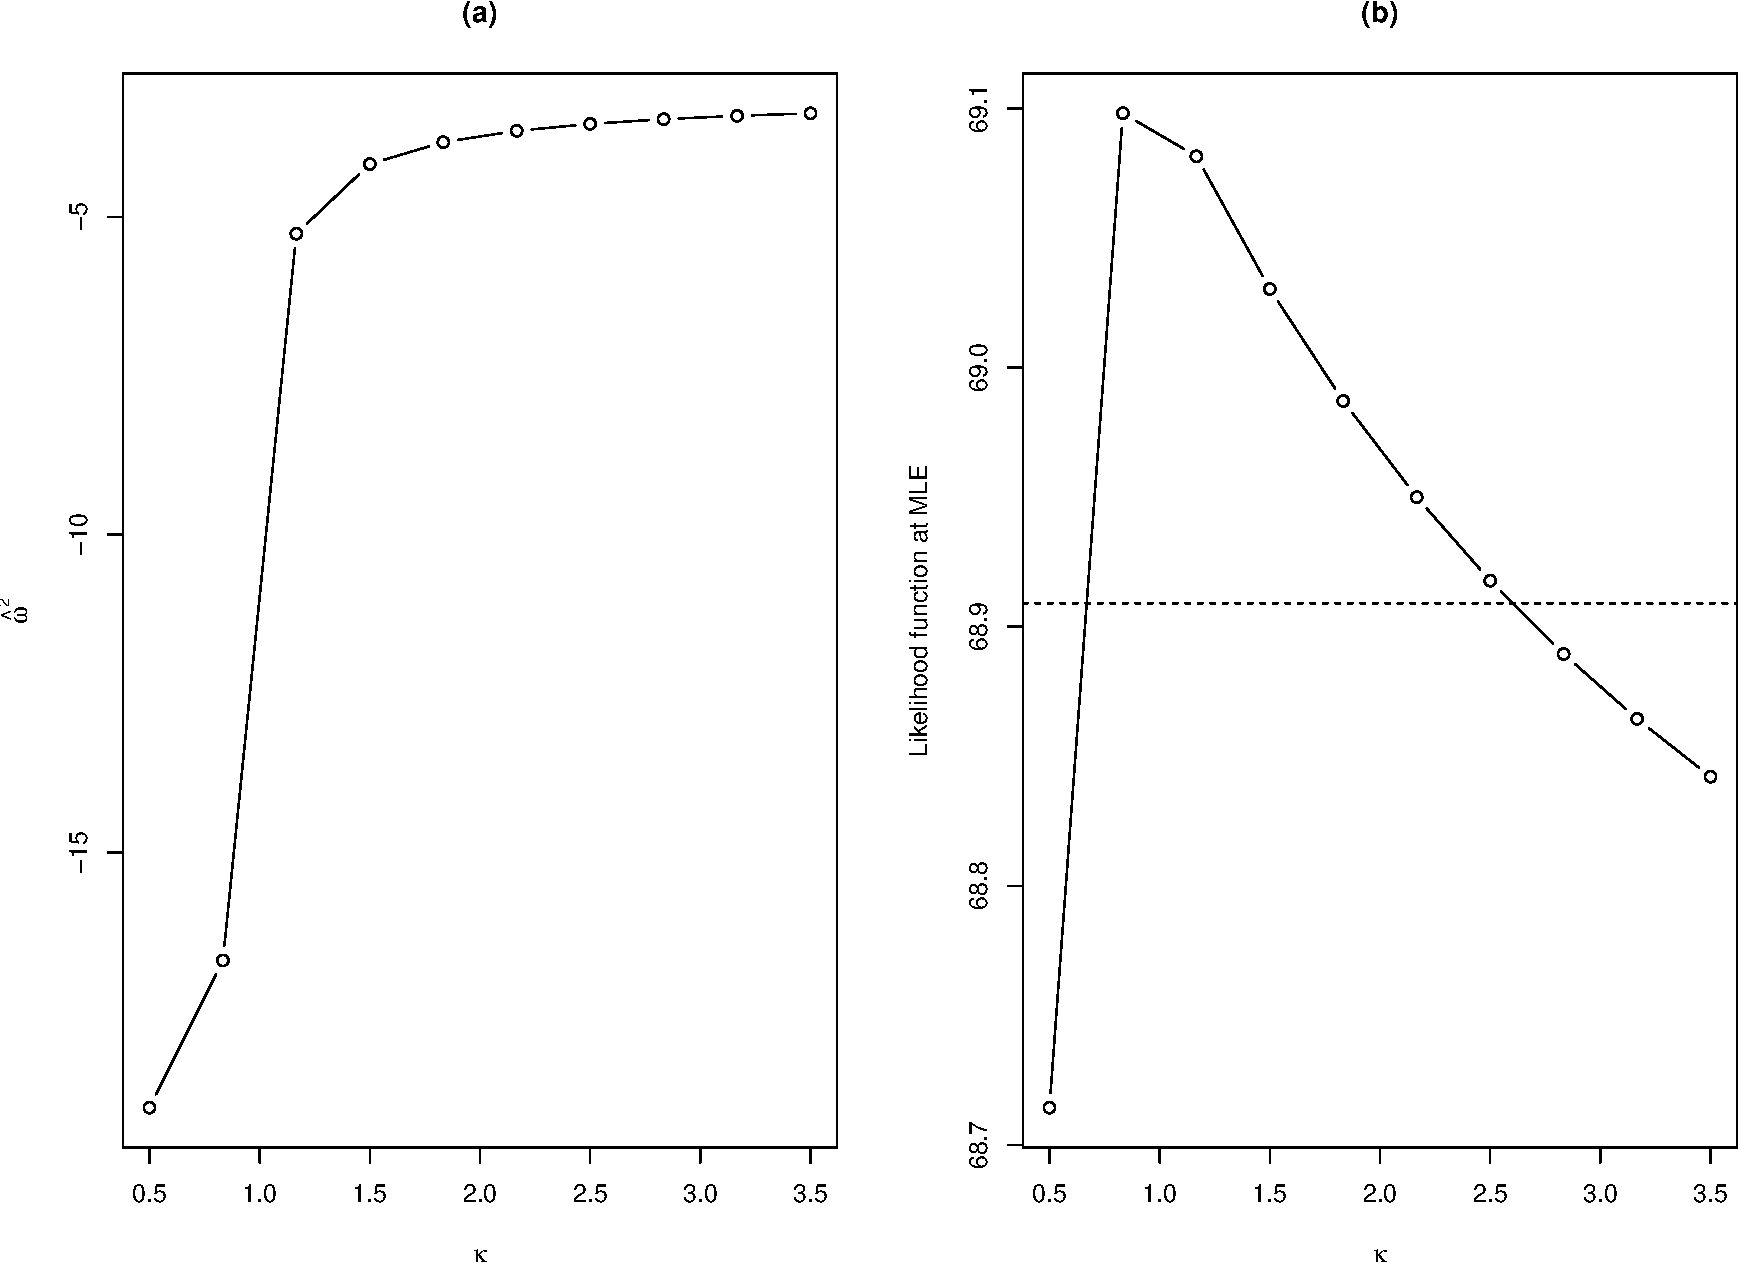
\includegraphics[width=8.5in,height=\textheight]{03_model-fitting_files/figure-pdf/fig-galicia-matern-1.pdf}

}

\caption{\label{fig-galicia-matern}(a) plot of the maximum likelihood
estimate for the variance of the measurement error \(U_i\), denoted in
the text as \(\omega^2\), against the chosen fixed value for \(\kappa\);
(b) profile likeihood for \(\kappa\) with the horizontal dashed line
corresponding to the (approximate) threshold for constructing a 95\%
confidence interval based on a \(\chi^2\) with one degree of freedom.}

\end{figure}

By examining the results shown in panel (a) of
Figure~\ref{fig-galicia-matern}, we observe that, as expected, smaller
values for \(\kappa\) leads to smaller point estimates for \(\omega^2\)
and viceversa. This begs the question, what should be our chosen value
for \(\kappa\)?

To answer this question, a natural approach is to estimate the model for
different values of \(\kappa\) and see which one give the best fit to
the data, according to the likelihood function. In panel (b) of
Figure~\ref{fig-galicia-matern}, we show the results of this approach
where we considered 10 values for \(\kappa\) within the range 0.5 to 3.5
(see code above). In this plot, we have also added a horizontal line to
help us to approximate a range of the most plausible value for
\(\kappa\). More precisely, the horizontal dashed line is computed by
taking the maximum observed values of the likelihoods computed for the
different values of \(\kappa\), say \(\hat{M}\) and we subtract the
quantile 0.95 of a \(\chi^2\) distribution with 1 degree of freedom. In
R this horizontal line is obtained as

\begin{Shaded}
\begin{Highlighting}[]
\FunctionTok{max}\NormalTok{(llik\_values)}\SpecialCharTok{{-}}\FunctionTok{pchisq}\NormalTok{(}\FloatTok{0.95}\NormalTok{, }\AttributeTok{df =} \DecValTok{2}\NormalTok{)}\SpecialCharTok{/}\DecValTok{2}
\end{Highlighting}
\end{Shaded}

where \texttt{llik\_values} is as defined in the previous chunk of code.
Note that this approach is essentially constructing the profile
likelihood for \(\kappa\) which one could use to derive a confidence
interval for \(\kappa\) with a finer segmentation for
\texttt{kappa\_values}. However, our current objective is not to derive
the confidence interval for \(\kappa\), but rather to gain a broad
understanding of the \(\kappa\) values supported by the dataset. The
values of \(\kappa\) that corresponds to likelihood values above the
horizontal line are approximately between 0.75 and 2.75. Hence,
selecting \(\kappa=1.5\) seems to be a reasonable one in this case. Now,
you may be pondering: are there value other than \(\kappa=1.5\) that
could fit the data even better? Our answer is that it is not worth the
effort to try estimate \(\kappa\) more precisely because it is
empirically very difficult and, under some scenarios, even impossible.
Estimating \(\kappa\) poses a well-documented challenge in geostatistics
(Zhang (2004)), which justifies our adoption of a pragmatic approach
that sets it at a predefined value. This issue is also further
exacerbated when analyzing count data, which tend to be less informative
about the correlation structure than continuously measured data.

\hypertarget{sec-add-re-glgm}{%
\subsection{\texorpdfstring{Modelling hierarchical geostatistical data
using the \texttt{re()}
function}{Modelling hierarchical geostatistical data using the re() function}}\label{sec-add-re-glgm}}

We now consider the analysis of geostatistical data with a hierarchical
structure and show how to formulate and fit a geostatistical model that
accounts for the effects of the different layers of the data. For this
purpose, we use the \texttt{italy\_sim} where each of the sampled
locations can be grouped according to two administrative subdivisions of
Italy, regions (Admin level 2) and provinces (Admin level 3), as shown
in Figure~\ref{fig-italy-maps}.

\begin{Shaded}
\begin{Highlighting}[]
\FunctionTok{library}\NormalTok{(rgeoboundaries)}
\FunctionTok{library}\NormalTok{(mapview)}
\NormalTok{italy\_regions }\OtherTok{\textless{}{-}} \FunctionTok{geoboundaries}\NormalTok{(}\AttributeTok{country =} \StringTok{"italy"}\NormalTok{, }\AttributeTok{adm\_lvl =} \StringTok{"adm2"}\NormalTok{)}

\NormalTok{italy\_provinces }\OtherTok{\textless{}{-}} \FunctionTok{geoboundaries}\NormalTok{(}\AttributeTok{country =} \StringTok{"italy"}\NormalTok{, }\AttributeTok{adm\_lvl =} \StringTok{"adm3"}\NormalTok{)}

\FunctionTok{par}\NormalTok{(}\AttributeTok{mfrow =} \FunctionTok{c}\NormalTok{(}\DecValTok{1}\NormalTok{,}\DecValTok{2}\NormalTok{))}

\CommentTok{\# Map of the data with the region boundaries}
\NormalTok{map\_regions }\OtherTok{\textless{}{-}} \FunctionTok{ggplot}\NormalTok{() }\SpecialCharTok{+} 
\FunctionTok{geom\_sf}\NormalTok{(}\AttributeTok{data =}\NormalTok{ italy\_sim\_sf, }\AttributeTok{pch =} \DecValTok{4}\NormalTok{, }\AttributeTok{color =} \StringTok{"red"}\NormalTok{) }\SpecialCharTok{+} 
\FunctionTok{geom\_sf}\NormalTok{(}\AttributeTok{data =}\NormalTok{ italy\_regions, }\AttributeTok{fill =} \ConstantTok{NA}\NormalTok{) }\SpecialCharTok{+} 
\FunctionTok{theme\_void}\NormalTok{() }\SpecialCharTok{+}
\FunctionTok{labs}\NormalTok{(}\AttributeTok{title =} \StringTok{"Regions"}\NormalTok{) }\SpecialCharTok{+}
\FunctionTok{theme}\NormalTok{(}\AttributeTok{plot.title =} \FunctionTok{element\_text}\NormalTok{(}\AttributeTok{hjust =} \DecValTok{1}\SpecialCharTok{/}\DecValTok{2}\NormalTok{))}

\CommentTok{\# Map of the data with the province boundaries}
\NormalTok{map\_provinces }\OtherTok{\textless{}{-}} \FunctionTok{ggplot}\NormalTok{() }\SpecialCharTok{+} 
\FunctionTok{geom\_sf}\NormalTok{(}\AttributeTok{data =}\NormalTok{ italy\_sim\_sf, }\AttributeTok{pch =} \DecValTok{4}\NormalTok{, }\AttributeTok{color =} \StringTok{"red"}\NormalTok{) }\SpecialCharTok{+} 
\FunctionTok{geom\_sf}\NormalTok{(}\AttributeTok{data =}\NormalTok{ italy\_provinces, }\AttributeTok{fill =} \ConstantTok{NA}\NormalTok{) }\SpecialCharTok{+} 
\FunctionTok{theme\_void}\NormalTok{() }\SpecialCharTok{+}
\FunctionTok{labs}\NormalTok{(}\AttributeTok{title =} \StringTok{"Provinces"}\NormalTok{) }\SpecialCharTok{+}
\FunctionTok{theme}\NormalTok{(}\AttributeTok{plot.title =} \FunctionTok{element\_text}\NormalTok{(}\AttributeTok{hjust =} \DecValTok{1}\SpecialCharTok{/}\DecValTok{2}\NormalTok{))}

\FunctionTok{library}\NormalTok{(gridExtra)}
\FunctionTok{grid.arrange}\NormalTok{(map\_regions, map\_provinces, }\AttributeTok{ncol =} \DecValTok{2}\NormalTok{)}
\end{Highlighting}
\end{Shaded}

\begin{figure}[H]

{\centering 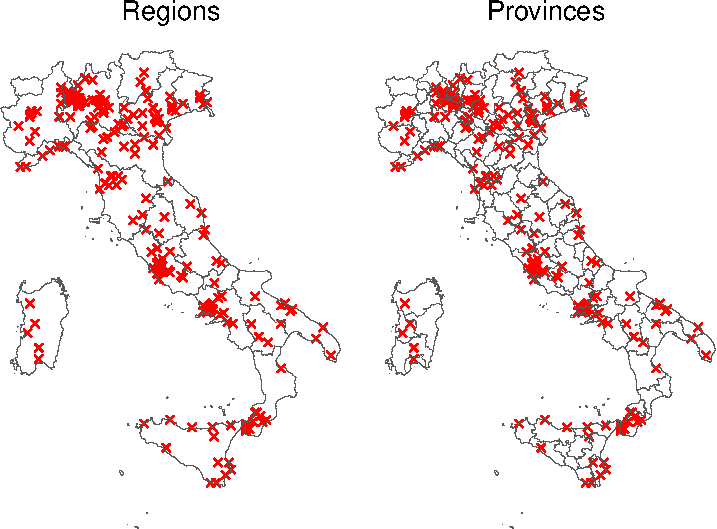
\includegraphics{03_model-fitting_files/figure-pdf/fig-italy-maps-1.pdf}

}

\caption{\label{fig-italy-maps}The plot shows the location of the
data-set \texttt{italy\_sim} (red crosses), with the boundaries of the
regions (left) and provinces (right) of Italy.}

\end{figure}

Let \(V_h\), for \(h=1,\ldots,n_V\) and \(Z_k\), for
\(k=1,\ldots,n_{Z}\), be a set of mutually independent Gaussian
variables with zero means and variances \(\sigma^2_{V}\) and
\(\sigma^2_{Z}\), respectively. Finally let \(\mathcal{A}_h\), for
\(h=1,\ldots,n_V\) and \(\mathcal{B}_k\), for \(k=1,\ldots,n_{Z}\),
denote the areas encompassed by the boundaries of the region and
provinces, respectively. Since we have 10 repeated observations at each
locations, we shall use \(Y_{ij}\) to denote the \(j\)-th outcome (found
in the data under the column \texttt{y}) at the \(i\)-th location
\(x_i\). The model from which we generated data \(y_{ij}\) is
\begin{equation}\protect\hypertarget{eq-italy-sim-model}{}{
Y_{ij} = \beta_0 + \overbrace{\beta_1 d(x_i) + S(x_i)}^\text{Location-level effect} + \underbrace{\sum_{h=1}^{n_{V}} I(x_i \in \mathcal{A}_h) \times V_h}_\text{Region effect} +\\ \overbrace{\sum_{k=1}^{n_{Z}} I(x_i \in \mathcal{B}_k) \times Z_k}^\text{Province effect} +  \underbrace{U_{ij}}_\text{Measurement error},
}\label{eq-italy-sim-model}\end{equation} for \(j=1,\ldots 10\) and
\(i=1,\ldots,200\), where, \(d(x_i)\) is the log-transformed population
density, \(I(x \in \mathcal{R})\) is an indicator function that takes
value 1 if the location \(x\) falls within the boundaries of the area
denoted by \(\mathcal{R}\) and 0 otherwise. The covariance function
chosen in the generation of the data was an exponential correlation
function hence
\({\rm cov}\{S(x), S(x') = \sigma^2 \exp\{-||x-x'||/\phi\}\).

The inclusion of the random effects \(V_h\), for the region, and
\(Z_k\), for the province, can be included by using the \texttt{re()}
function into the \texttt{formula} passed to \texttt{glgpm} as shown
below.

\begin{Shaded}
\begin{Highlighting}[]

                        \CommentTok{\# Location{-}level effect}
\NormalTok{italy\_fit }\OtherTok{\textless{}{-}} \FunctionTok{glgpm}\NormalTok{( y }\SpecialCharTok{\textasciitilde{}} \FunctionTok{log}\NormalTok{(pop\_dens) }\SpecialCharTok{+} \FunctionTok{gp}\NormalTok{(}\AttributeTok{kappa =} \FloatTok{0.5}\NormalTok{, }\AttributeTok{nugget =} \DecValTok{0}\NormalTok{) }\SpecialCharTok{+}
                        \CommentTok{\# Region and province effects}
                        \FunctionTok{re}\NormalTok{(region, province),}
         \AttributeTok{data =}\NormalTok{ italy\_sim\_sf, }\AttributeTok{scale\_to\_km =} \ConstantTok{TRUE}\NormalTok{,}
         \AttributeTok{family =} \StringTok{"gaussian"}\NormalTok{)}
\DocumentationTok{\#\# The CRS used is EPSG:32634 }
\DocumentationTok{\#\# Distances between locations are computed in kilometers }
\DocumentationTok{\#\#   0:     441.00731: {-}0.404481  1.33798  0.00000  4.62406  0.00000  0.00000  0.00000}
\DocumentationTok{\#\#   1:    {-}130.05497: {-}0.408825  1.35003 {-}0.0387110  4.66059 {-}0.910409 {-}0.00265292 0.0107965}
\DocumentationTok{\#\#   2:    {-}268.13436: {-}0.865126  1.39525 {-}0.0305268  5.92133 {-}1.96079 {-}0.666581 0.487537}
\DocumentationTok{\#\#   3:    {-}329.24560: {-}1.44091  1.38139 {-}0.546306  4.98616 {-}1.67936 {-}1.15202 0.383821}
\DocumentationTok{\#\#   4:    {-}331.20861: {-}1.38498  1.37256 0.165464  5.61366 {-}1.63033 {-}2.11435 0.371263}
\DocumentationTok{\#\#   5:    {-}331.28418: {-}0.874796  1.37322 {-}0.271990  5.18071 {-}1.62887 {-}0.970705 0.371407}
\DocumentationTok{\#\#   6:    {-}331.42968: {-}1.04087  1.37294 {-}0.119652  5.33634 {-}1.62883 {-}1.33321 0.375031}
\DocumentationTok{\#\#   7:    {-}331.43375: {-}1.07312  1.37288 {-}0.0878211  5.36725 {-}1.62883 {-}1.42011 0.376251}
\DocumentationTok{\#\#   8:    {-}331.43375: {-}1.07445  1.37288 {-}0.0866254  5.36840 {-}1.62883 {-}1.42489 0.376323}
\DocumentationTok{\#\#   9:    {-}331.43375: {-}1.07445  1.37288 {-}0.0866228  5.36840 {-}1.62883 {-}1.42491 0.376323}
\DocumentationTok{\#\#  10:    {-}331.43375: {-}1.07445  1.37288 {-}0.0866227  5.36840 {-}1.62883 {-}1.42491 0.376323}
\DocumentationTok{\#\#  11:    {-}331.43375: {-}1.07445  1.37288 {-}0.0866227  5.36840 {-}1.62883 {-}1.42491 0.376323}

\FunctionTok{summary}\NormalTok{(italy\_fit)}
\DocumentationTok{\#\# Linear geostatsitical model }
\DocumentationTok{\#\# \textquotesingle{}Lower limit\textquotesingle{} and \textquotesingle{}Upper limit\textquotesingle{} are the limits of the 95\% confidence level intervals }
\DocumentationTok{\#\# }
\DocumentationTok{\#\#  Regression coefficients }
\DocumentationTok{\#\#                Estimate Lower limit Upper limit    StdErr z.value p.value    }
\DocumentationTok{\#\# (Intercept)   {-}1.074454   {-}2.031694   {-}0.117213  0.488397    {-}2.2 0.02781 *  }
\DocumentationTok{\#\# log(pop\_dens)  1.372877    1.352018    1.393735  0.010642   129.0 \textless{} 2e{-}16 ***}
\DocumentationTok{\#\# {-}{-}{-}}
\DocumentationTok{\#\# Signif. codes:  0 \textquotesingle{}***\textquotesingle{} 0.001 \textquotesingle{}**\textquotesingle{} 0.01 \textquotesingle{}*\textquotesingle{} 0.05 \textquotesingle{}.\textquotesingle{} 0.1 \textquotesingle{} \textquotesingle{} 1}
\DocumentationTok{\#\# }
\DocumentationTok{\#\#                          Estimate Lower limit Upper limit}
\DocumentationTok{\#\# Measuremment error var.  0.19616     0.19361      0.1987}
\DocumentationTok{\#\# }
\DocumentationTok{\#\#  Spatial Guassian process }
\DocumentationTok{\#\# Matern covariance parameters (kappa=0.5) }
\DocumentationTok{\#\#                       Estimate Lower limit Upper limit}
\DocumentationTok{\#\# Spatial process var.   0.91702     0.59470       1.414}
\DocumentationTok{\#\# Spatial corr. scale  214.52032   153.60797     299.587}
\DocumentationTok{\#\# Variance of the nugget effect fixed at 0 }
\DocumentationTok{\#\# }
\DocumentationTok{\#\#  Unstructured random effects }
\DocumentationTok{\#\#                             Estimate Lower limit Upper limit}
\DocumentationTok{\#\# region (random eff. var.)    0.24053     0.14553      0.3976}
\DocumentationTok{\#\# province (random eff. var.)  1.45692     1.37851      1.5398}
\DocumentationTok{\#\# }
\DocumentationTok{\#\#  Log{-}likelihood: 331.4338}
\DocumentationTok{\#\# }
\DocumentationTok{\#\#  AIC: {-}662.8675}
\DocumentationTok{\#\# }
\end{Highlighting}
\end{Shaded}

In the code above, the \texttt{factor} variables \texttt{region} and
\texttt{province} found in \texttt{italy\_sim} are passed to
\texttt{re()} and these are estimated as unstructured random effects as
defined by Equation~\ref{eq-italy-sim-model}. From the summary of model,
we then obtain the parameter and interval estimates as reported in
Table~\ref{tbl-italy-sim-mle}.

\hypertarget{tbl-italy-sim-mle}{}
\begin{longtable}[]{@{}llll@{}}
\caption{\label{tbl-italy-sim-mle}Maximum likelihood estimates and,
lower and upper limits of the 95\% confidence interval for the
parameters of the model in
Equation~\ref{eq-italy-sim-lmm}.}\tabularnewline
\toprule\noalign{}
Parameter & Point estimate & Lower limit & Upper limit \\
\midrule\noalign{}
\endfirsthead
\toprule\noalign{}
Parameter & Point estimate & Lower limit & Upper limit \\
\midrule\noalign{}
\endhead
\bottomrule\noalign{}
\endlastfoot
\(\beta_0\) & -1.074 & -2.032 & -0.117 \\
\(\beta_1\) & 1.373 & 1.352 & 1.394 \\
\(\sigma^2\) & 0.917 & 0.595 & 1.414 \\
\(\phi\) & 214.520 & 153.608 & 299.587 \\
\(\sigma^2_{V}\) & 0.241 & 0.146 & 0.398 \\
\(\sigma^2_{Z}\) & 1.457 & 1.379 & 1.540 \\
\(\omega^2\) & 0.196 & 0.194 & 0.199 \\
\end{longtable}

The function \texttt{to\_table} from the \texttt{RiskMap} package can be
used to obtain the Latex or HTML code directly from a fit of the model.
Here is an example.

\begin{Shaded}
\begin{Highlighting}[]
\FunctionTok{to\_table}\NormalTok{(italy\_fit, }\AttributeTok{digits =} \DecValTok{3}\NormalTok{)}
\DocumentationTok{\#\# \% latex table generated in R 4.1.2 by xtable 1.8{-}4 package}
\DocumentationTok{\#\# \% Thu Feb  1 16:23:10 2024}
\DocumentationTok{\#\# \textbackslash{}begin\{table\}[ht]}
\DocumentationTok{\#\# \textbackslash{}centering}
\DocumentationTok{\#\# \textbackslash{}begin\{tabular\}\{rrrr\}}
\DocumentationTok{\#\#   \textbackslash{}hline}
\DocumentationTok{\#\#  \& Estimate \& Lower limit \& Upper limit \textbackslash{}\textbackslash{} }
\DocumentationTok{\#\#   \textbackslash{}hline}
\DocumentationTok{\#\# (Intercept) \& {-}1.074 \& {-}2.032 \& {-}0.117 \textbackslash{}\textbackslash{} }
\DocumentationTok{\#\#   log(pop\textbackslash{}\_dens) \& 1.373 \& 1.352 \& 1.394 \textbackslash{}\textbackslash{} }
\DocumentationTok{\#\#   Spatial process var. \& 0.917 \& 0.595 \& 1.414 \textbackslash{}\textbackslash{} }
\DocumentationTok{\#\#   Spatial corr. scale \& 214.520 \& 153.608 \& 299.587 \textbackslash{}\textbackslash{} }
\DocumentationTok{\#\#   region (random eff. var.) \& 0.241 \& 0.146 \& 0.398 \textbackslash{}\textbackslash{} }
\DocumentationTok{\#\#   province (random eff. var.) \& 1.457 \& 1.379 \& 1.540 \textbackslash{}\textbackslash{} }
\DocumentationTok{\#\#   Measuremment error var. \& 0.196 \& 0.194 \& 0.199 \textbackslash{}\textbackslash{} }
\DocumentationTok{\#\#    \textbackslash{}hline}
\DocumentationTok{\#\# \textbackslash{}end\{tabular\}}
\DocumentationTok{\#\# \textbackslash{}end\{table\}}
\end{Highlighting}
\end{Shaded}

\hypertarget{generalized-linear-geostatistical-models}{%
\section{Generalized linear geostatistical
models}\label{generalized-linear-geostatistical-models}}

We now consider the modelling of count outcomes, focusing our attention
to the Binomial and Poisson geostatistical models.

The use of Binomial geostatistical model is appropriate whenever the
reported counts have a known upper bound. For example, when analyzing
aggregated disease counts from cross-sectional survey data, the total
number of people sampled at a location defines the largest number of
possible reported disease cases. Recalling the model specification of
Table~\ref{tbl-glm}, we specify the Binomial geostatistical model by
stating that the reported disease counts \(Y_i\) out of \(n_i\) (the
maximum value that \(Y_i\) can take) at location \(x_i\), conditionally
on the spatial random effects \(S(x_i)\), follow a Binomial distribution
with probability \(p(x_i)\) and logit-linear predictor
\begin{equation}\protect\hypertarget{eq-lp-bin}{}{
\log\left\{\frac{p(x_i)}{1-p(x_i)}\right\} = d(x_i)^\top \beta + S(x_i).
}\label{eq-lp-bin}\end{equation} In this model, \(p(x_i)\) is commonly
understood as representing the prevalence of the disease under
consideration, defined as the proportion of individuals with the disease
at a specific moment. While \(p(x_i)\) is not strictly a proportion, its
interpretation as disease prevalence is justified by the fact that if we
were to sample a sufficiently large population at location \(x_i\), the
proportion of individuals with the disease would converge closely to the
value of \(p(x_i)\).

A Binomial geostatistical model is also used when analyzing data at
individual level where the outcome is binary and usually indicates the
positive or negative result of a test for a disease under investigation.
In this analysis, a mix of individual-level variables and location-level
variables could be introduced to model the probability of a positive
test. To formally write the model, we now use \(Y_{ij}\) to indicate the
binary outcome taking value 1, if the test was positive, and 0, if
negative, for the \(j\)-th individual sampled at location \(x_i\). The
linear predictor now takes the form
\begin{equation}\protect\hypertarget{eq-lp-bin-ind}{}{
\log\left\{\frac{p_{ij}}{1-p_{ij}}\right\} = e_{ij}^\top \gamma + d(x_{i})^\top \beta + S(x_i).
}\label{eq-lp-bin-ind}\end{equation} In the model above we have
distinguished between covariates \(e_{ij}\), that express the effect on
\(p_{ij}\) due to individual traits (such as age and gender), and
covariates \(d(x_i)\), that instead quantify the effect on \(p_{ij}\)
resulting from the environmental attributes of location \(x_i\) (such as
elevation, temperature, and precipitation). In this model \(p_{ij}\) --
the probability of a positive test -- once again can be interpreted as
the disease prevalence for a population characterized by the individual
traits \(e_{ij}\) and residing at location \(x_i\).

Finally, when the counts arise from a population whose size is unknown
or when the occurrence of a disease is very small relative to the size
of the target population, one should consider the use of a Poisson
geostaistical model. We then use \(Y_i\) to denote the reported counts
at location \(x_i\) and assume that this, conditionally on a Gaussian
process \(S(x_i)\), follows a Poisson distribution with mean
\(\lambda(x_i)\) and log-linear predictor
\begin{equation}\protect\hypertarget{eq-poisson-lp}{}{
\log\left\{\lambda(x_i)\right\} = d(x_i)^\top \beta + S(x_i). 
}\label{eq-poisson-lp}\end{equation} If for example, \(Y_i\) corresponds
to the number of new cases reported at a health facility at location
\(x_i\) over a certain, the \(\lambda(x_i)\) is interpreted as the
average number of new cases reported over that period. If the
information on the size of the population at risk for the diseases were
available, this can be incorporated into the model so as to enable the
interpretation of \(\lambda(x_i)\) as the disease incidence, defined as
the total number of new cases reported over a given period of time
divided by the population at risk. If we denote the latter as \(m_i\),
then we would specify the mean of \(Y_i\) as \(m_i\lambda(x_i)\) an
model \(\lambda(x_i)\) as already specified in
Equation~\ref{eq-poisson-lp}. Another prevalent application of the
Poisson geostatistical model in epidemiology involves mapping the
abundance of disease vectors. Here, \(\lambda(x_i)\) corresponds to the
mean number of vectors per unit area. Also, note that in this last
scenario \(m_i\) cannot be defined as it is the goal of the analysis to
infer the vector population size at location \(x_i\).

In all the three models, namely Equation~\ref{eq-lp-bin},
Equation~\ref{eq-lp-bin-ind} and Equation~\ref{eq-poisson-lp}, one might
consider the inclusion of an additional random effect \(Z_i\),
previously used for the linear geostatistical model, to account for
small spatial variation or overdispersion that stems from the omission
of covariates that may not necessarily exhibit spatial structure, such
as behavioral or genetic traits. We shall further elaborate and provide
guidance on this point in the following examples of this section.

\hypertarget{theory}{%
\section{Theory}\label{theory}}

\hypertarget{the-likelihood-function-of-a-genearlized-linear-mixed-model}{%
\subsection{The likelihood function of a genearlized linear mixed
model}\label{the-likelihood-function-of-a-genearlized-linear-mixed-model}}

\hypertarget{the-likelihood-function-of-a-genearlized-linear-geostatistical-model}{%
\subsection{The likelihood function of a genearlized linear
geostatistical
model}\label{the-likelihood-function-of-a-genearlized-linear-geostatistical-model}}

\hypertarget{monte-carlo-maximum-likelihood}{%
\subsection{Monte Carlo maximum
likelihood}\label{monte-carlo-maximum-likelihood}}

\hypertarget{exercises}{%
\section{Exercises}\label{exercises}}

\begin{enumerate}
\def\labelenumi{\arabic{enumi}.}
\setcounter{enumi}{1}
\item
  Consider the Binomial mixed model with linear predictor as defined in
  Equation~\ref{eq-linear-predictor-glmms-ch2}. By editing the code for
  the simulation shown in Section~\ref{sec-overdispersion}, generate a
  graph as in Figure~\ref{fig-var-bin-glmm} under the two following
  scenarios: \(i\)) \(\tau^2 = 0.2\) and \(n_i=100\); \(ii\))
  \(\tau^2 = 0.1\) and \(n_i = 1\). How does the variance of \(Y_i\)
  change under \(i\)) and \(ii\)) in comparison to
  Figure~\ref{fig-var-bin-glmm}? How do you explain the differences?
\item
  Similarly to the previous exercise, consider a Poisson mixed model
  with linear predictor \[
  \log\left\{\mu_i\right\} = \beta_0 + Z_i,
  \] where \(Z_i\) are a set of mutually independent Gaussian variables
  with mean 0 and variance \(\tau^2\). Using the code shown in
  Section~\ref{sec-overdispersion}, carry out a simulation study to
  compute the variance of \(Y_i\) and generate a graph similar to
  Figure~\ref{fig-var-bin-glmm} to compare the variance of the Poisson
  mixed model with that of a standard Poisson model. Generate the graph
  for different values of \(\tau^2\) and summarize your findings. NOTE:
  In this simulation the offset \(n_i\) can be set to 1.
\item
  Create an R function that computes the \emph{cloud variogram}. As
  explained in Section~\ref{sec-expl-spatial}, the cloud variogram is
  obtained by plotting \(\hat{V}_{ij}\) (see
  Equation~\ref{eq-hat-squared-diff}) against the distances \(u_{ij}\).
  The function should take as input a data-set with three columns: the
  variable for which the cloud variogram is to be computed; and two
  columns corresponding to the location of the data. Then, use this
  function to create the cloud variogram for the model for
  river-blindness in Equation~\ref{eq-liberia-bin-mixed-elev}. How does
  this compare to empirical variogram that takes the averages within
  predefined distance classes, as shown in
  Figure~\ref{fig-liberia-variog}?
\item
  Fit a Binomial mixed model to the Liberia data-set on river-blindness
  without any covariates, i.e.~\[
  \log\left\{\frac{p(x_i)}{1-p(x_i)}\right\} = \beta_0 + Z_i.
  \] Making use of the R code presented in
  Section~\ref{sec-empirical-variog-bin}, use the function
  \texttt{s\_variogram} to generate the empirical variogram for this
  model and compare this to the empirical variogram of
  Figure~\ref{fig-liberia-variog}. What differences do you observe?
\item
  Fit a Poisson mixed model to the anopheles mosquito data using
  elevation as a covariate, i.e.~\[
  \log\{\mu(x_i)\} = \beta_{0} + \beta_{1} d(x_i) + Z_i
  \] where \(d(x_i)\) is the measured elevation at location \(x_i\). How
  strong is the overdispersion in the data? After fitting the model,
  extract the estimates of the random effects \(Z_i\) and compute the
  empirical variogram with the 95\% envelope for spatial independence.
  Repeat this for different classes of distances by changing the input
  passed to \texttt{bins} in the \texttt{s\_variogram} function. How do
  the different specifications of \texttt{bins} affect the results?
\item
  Consider a linear model for the Galicia data as in
  Section~\ref{sec-glm-parest} but now also introduce a nugget term,
  hence \begin{equation}\protect\hypertarget{eq-galicia-lgm-v2}{}{
  Y_i = \mu + S(x_i) + Z_i + U_i
  }\label{eq-galicia-lgm-v2}\end{equation} where \(Z_i\) are i.i.d.
  Gaussian variables with mean 0 and variance \(\tau^2\). Fit the model
  by fixing the variance of \(U_i\), \(\omega^2\) to 0.01 using the
  argument \texttt{fix\_var\_me} in \texttt{glgpm}. Using this model,
  reproduce the graph as shown in Figure~\ref{fig-galicia-matern}.
  Repeat this, but now fix \(\omega^2\) to 0.02. How do the curves
  change and why?
\end{enumerate}

\bookmarksetup{startatroot}

\hypertarget{sec-validation}{%
\chapter{Model validation}\label{sec-validation}}

This is a book created from markdown and executable code.

See (\textbf{knuth84?}) for additional discussion of literate
programming.

\begin{Shaded}
\begin{Highlighting}[]
\DecValTok{1} \SpecialCharTok{+} \DecValTok{1}
\end{Highlighting}
\end{Shaded}

\begin{verbatim}
[1] 2
\end{verbatim}

\hypertarget{how-to-simulate-geostatistical-data-from-a-fitted-model}{%
\section{How to simulate geostatistical data from a fitted
model}\label{how-to-simulate-geostatistical-data-from-a-fitted-model}}

\hypertarget{validating-the-calibration-of-the-model}{%
\section{Validating the calibration of the
model}\label{validating-the-calibration-of-the-model}}

\hypertarget{validating-the-spatial-correlation-of-the-model}{%
\section{Validating the spatial correlation of the
model}\label{validating-the-spatial-correlation-of-the-model}}

\bookmarksetup{startatroot}

\hypertarget{sec-geo-prediction}{%
\chapter{Geostatistical prediction}\label{sec-geo-prediction}}

This is a book created from markdown and executable code.

See (\textbf{knuth84?}) for additional discussion of literate
programming.

\begin{Shaded}
\begin{Highlighting}[]
\DecValTok{1} \SpecialCharTok{+} \DecValTok{1}
\end{Highlighting}
\end{Shaded}

\begin{verbatim}
[1] 2
\end{verbatim}

\hypertarget{pixel-level-predictive-targets}{%
\section{Pixel-level predictive
targets}\label{pixel-level-predictive-targets}}

\hypertarget{area-level-predictive-targets}{%
\section{Area-level predictive
targets}\label{area-level-predictive-targets}}

\hypertarget{comparing-the-predictive-performance-of-geostatistical-models}{%
\section{Comparing the predictive performance of geostatistical
models}\label{comparing-the-predictive-performance-of-geostatistical-models}}

\bookmarksetup{startatroot}

\hypertarget{sec-case-studies}{%
\chapter{Case studies}\label{sec-case-studies}}

This is a book created from markdown and executable code.

See (\textbf{knuth84?}) for additional discussion of literate
programming.

\begin{Shaded}
\begin{Highlighting}[]
\DecValTok{1} \SpecialCharTok{+} \DecValTok{1}
\end{Highlighting}
\end{Shaded}

\begin{verbatim}
[1] 2
\end{verbatim}

\hypertarget{mapping-stunting-risk-in-ghan}{%
\section{Mapping stunting risk in
Ghan}\label{mapping-stunting-risk-in-ghan}}

\hypertarget{mapping-river-blindness-in-malawi}{%
\section{Mapping river blindness in
Malawi}\label{mapping-river-blindness-in-malawi}}

\hypertarget{mapping-mosquitoes-abundance-in-cameroon}{%
\section{Mapping mosquitoes abundance in
Cameroon}\label{mapping-mosquitoes-abundance-in-cameroon}}

\bookmarksetup{startatroot}

\hypertarget{references}{%
\chapter*{References}\label{references}}
\addcontentsline{toc}{chapter}{References}

\markboth{References}{References}

\hypertarget{refs}{}
\begin{CSLReferences}{1}{0}
\leavevmode\vadjust pre{\hypertarget{ref-bates2015}{}}%
Bates, Douglas, Martin Mächler, Ben Bolker, and Steve Walker. 2015.
{``Fitting Linear Mixed-Effects Models Using {lme4}.''} \emph{Journal of
Statistical Software} 67 (1): 1--48.
\url{https://doi.org/10.18637/jss.v067.i01}.

\leavevmode\vadjust pre{\hypertarget{ref-bowman1997}{}}%
Bowman, A. W. 1997. \emph{Applied Smoothing Techniques for Data Analysis
: The Kernel Approach with s-Plus Illustrations}. Oxford Statistical
Science Series ; 18. Oxford : New York: Clarendon Press ; Oxford
University Press.

\leavevmode\vadjust pre{\hypertarget{ref-breslow1993}{}}%
Breslow, N. E., and D. G. Clayton. 1993. {``Approximate Inference in
Generalized Linear Mixed Models.''} \emph{Journal of the American
Statistical Association} 88: 9--25.

\leavevmode\vadjust pre{\hypertarget{ref-chilesdelfiner2016}{}}%
Chilès, J-P, and P. Delfiner. 2016. \emph{Geostatistics (Second
Edition)}. Hoboken: Wiley.

\leavevmode\vadjust pre{\hypertarget{ref-cressie1991}{}}%
Cressie, N. A. C. 1991. \emph{Statistics for Spatial Data}. New York:
Wiley.

\leavevmode\vadjust pre{\hypertarget{ref-diggle1998}{}}%
Diggle, P. J., J. A. Tawn, and R. A. Moyeed. 1998. {``Model-Based
Geostatistics.''} \emph{Journal of the Royal Statistical Society: Series
C (Applied Statistics)} 47 (3): 299--350.
\url{https://doi.org/10.1111/1467-9876.00113}.

\leavevmode\vadjust pre{\hypertarget{ref-diggleBook2019}{}}%
Diggle, Peter J. 2019. \emph{Model-Based Geostatistics for Global Public
Health : Methods and Applications.} Chapman and Hall/CRC
Interdisciplinary Statistics Ser. Milton: Chapman; Hall/CRC.

\leavevmode\vadjust pre{\hypertarget{ref-dobson2008}{}}%
Dobson, A. J., and A. Barnett. 2008. \emph{An Introduction to
Generalized Linear Models}. Third. Chapman; Hall/CRC.

\leavevmode\vadjust pre{\hypertarget{ref-fernandez2000}{}}%
Fernández, J. A, A Rey, and A Carballeira. 2000. {``An Extended Study of
Heavy Metal Deposition in Galicia (NW Spain) Based on Moss Analysis.''}
\emph{Science of The Total Environment} 254 (1): 31--44.
\url{https://doi.org/10.1016/S0048-9697(00)00431-9}.

\leavevmode\vadjust pre{\hypertarget{ref-hastie2001}{}}%
Hastie, Trevor, Robert Tibshirani, and Jerome Friedman. 2001. \emph{The
Elements of Statistical Learning}. Springer Series in Statistics. New
York, NY, USA: Springer New York Inc.

\leavevmode\vadjust pre{\hypertarget{ref-gates2020}{}}%
Katz, Elizabeth, and Bill \& Melinda Gates Foundation. 2020. {``Gender
and Malaria Evidence Reivew.''} Bill \& Melinda Gates Foundation.
\url{https://www.gatesgenderequalitytoolbox.org/wp-content/uploads/BMGF_Malaria-Review_FC.pdf}.

\leavevmode\vadjust pre{\hypertarget{ref-krige1951}{}}%
Krige, D. G. 1951. {``A Statistical Approach to Some Basic Mine
Valuation Problems on the Witwatersrand.''} \emph{Journal of the
Chemical, Metallurgical and Mining Society of South Africa} 52: 119--39.

\leavevmode\vadjust pre{\hypertarget{ref-matern2013}{}}%
Matern, B. 2013. \emph{Spatial Variation}. Lecture Notes in Statistics.
Springer New York.
\url{https://books.google.co.uk/books?id=HrbSBwAAQBAJ}.

\leavevmode\vadjust pre{\hypertarget{ref-matheron1963}{}}%
Matheron, G. 1963. {``Principles of Geostatistics.''} \emph{Economic
Geology} 58: 1246--66.

\leavevmode\vadjust pre{\hypertarget{ref-nelder1972}{}}%
Nelder, J. A., and R. W. M. Wedderburn. 1972. {``Generalized Linear
Models.''} \emph{Journal of the Royal Statistical Society A} 135:
370--84.

\leavevmode\vadjust pre{\hypertarget{ref-pawitan2001}{}}%
Pawitan, Yudi. 2001. \emph{In All Likelihood : Statistical Modelling and
Inference Using Likelihood}. Oxford ; New York: Clarendon Press : Oxford
University Press.

\leavevmode\vadjust pre{\hypertarget{ref-ripley1981}{}}%
Ripley, B. D. 1981. \emph{Spatial Statistics}. New York: Wiley.

\leavevmode\vadjust pre{\hypertarget{ref-ross2013}{}}%
Ross, Sheldon. 2013. \emph{First Course in Probability, a.} 9th ed.
Harlow: Pearson Education UK.

\leavevmode\vadjust pre{\hypertarget{ref-smith2007}{}}%
Smith, David L, Carlos A Guerra, Robert W Snow, and Simon I Hay. 2007.
{``Standardizing Estimates of the Plasmodium Falciparum Parasite
Rate.''} \emph{Malaria Journal} 6 (1): 131--31.

\leavevmode\vadjust pre{\hypertarget{ref-stein1999}{}}%
Stein, Michael L. 1999. \emph{Interpolation of Spatial Data Some Theory
for Kriging}. 1st ed. 1999. Springer Series in Statistics. New York, NY:
Springer New York : Imprint: Springer.

\leavevmode\vadjust pre{\hypertarget{ref-stevenson2013}{}}%
Stevenson, Gillian H. AND Gitonga, Jennifer C. AND Stresman. 2013.
{``Reliability of School Surveys in Estimating Geographic Variation in
Malaria Transmission in the Western Kenyan Highlands.''} \emph{PLOS ONE}
8 (10). \url{https://doi.org/10.1371/journal.pone.0077641}.

\leavevmode\vadjust pre{\hypertarget{ref-fossog2015}{}}%
Tene Fossog, Billy, Diego Ayala, Pelayo Acevedo, Pierre Kengne, Ignacio
Ngomo Abeso Mebuy, Boris Makanga, Julie Magnus, et al. 2015. {``Habitat
Segregation and Ecological Character Displacement in Cryptic African
Malaria Mosquitoes.''} \emph{Evolutionary Applications} 8 (4): 326--45.
\url{https://doi.org/10.1111/eva.12242}.

\leavevmode\vadjust pre{\hypertarget{ref-tobler1970}{}}%
Tobler, W. R. 1970. {``A Computer Movie Simulating Urban Growth in the
Detroit Region.''} \emph{Economic Geography} 46: 234--40.

\leavevmode\vadjust pre{\hypertarget{ref-watson1971}{}}%
Watson, G. S. 1971. {``Trend -Surface Analysis.''} \emph{Mathematical
Geology} 3: 215--26.

\leavevmode\vadjust pre{\hypertarget{ref-watson1972}{}}%
---------. 1972. {``Trend Surface Analysis and Spatial Correlation.''}
\emph{Geological Society of America Special Paper} 146: 39--46.

\leavevmode\vadjust pre{\hypertarget{ref-weisberg2014}{}}%
Weisberg, Sanford. 2014. \emph{Applied Linear Regression}. Fourth.
Hoboken {NJ}: Wiley. \url{http://z.umn.edu/alr4ed}.

\leavevmode\vadjust pre{\hypertarget{ref-zhang2004}{}}%
Zhang, Hao. 2004. {``Inconsistent Estimation and Asymptotically Equal
Interpolations in Model-Based Geostatistics.''} \emph{Journal of the
American Statistical Association} 99 (465): 250--61.

\leavevmode\vadjust pre{\hypertarget{ref-zoure2014}{}}%
Zouré, Honorat GM, Mounkaila Noma, Afework H Tekle, Uche V Amazigo,
Peter J Diggle, Emanuele Giorgi, and Jan HF Remme. 2014. {``Geographic
Distribution of Onchocerciasis in the 20 Participating Countries of the
African Programme for Onchocerciasis Control: (2) Pre-Control Endemicity
Levels and Estimated Number Infected.''} \emph{Parasites \& Vectors} 7
(1): 326--26.

\end{CSLReferences}



\end{document}
